%%% -*- Mode: LaTeX; -*-

%%%#+BEGIN: bx:dblock:global:this-file :disabledP "false" :mode "auto"
\begin{whenOrg}
*  #This File: /lcnt/lgpc/bystar/permanent/engineering/aiActivity_EmacsConf26/bodyPresArtEnFa.tex
\end{whenOrg}
%%%#+END:

%%%#+BEGIN: bx:dblock:lcnt:latex:inputed-title :disabledP "false" :mode "auto"
\begin{whenOrg}
* [[elisp:(show-all)][(>]] [[elisp:(describe-function 'org-dblock-write:bx:dblock:lcnt:latex:inputed-title)][dbf]]
*  [[elisp:(beginning-of-buffer)][Top]] ################  [[elisp:(delete-other-windows)][(1)]]   /*PLPC-180072 -- LCNT Panel -- lcntProc.sh, presProc.sh and Mailings*/
*  [[elisp:(beginning-of-buffer)][Top]] ################  [[elisp:(delete-other-windows)][(1)]]   *Beyond the Chatbot: Team-Oriented AI in Emacs*
*  [[elisp:(beginning-of-buffer)][Top]] ################  [[elisp:(delete-other-windows)][(1)]]   http://www.by-star.net/PLPC/180072
*  [[elisp:(beginning-of-buffer)][Top]] ################  [[elisp:(delete-other-windows)][(1)]]   [[elisp:(find-file "presentationEnFa.ttytex")][Visit ./presentationEnFa.ttytex]] || [[elisp:(find-file "articleEnFa.ttytex")][Visit ./articleEnFa.ttytex]] || [[elisp:(find-file "presArtEnFa.ttytex")][Visit ./presArtEnFa.ttytex]] ||

* [[elisp:(org-shifttab)][<)]] [[elisp:(describe-function 'org-dblock-write:bx:dblock:lcnt:latex:inputed-title)][dbFunc)]]  E|
\end{whenOrg}
%%%#+END:

%%%#+BEGIN: bx:dblock:global:org-controls :disabledP "false" :mode "auto"
\begin{whenOrg}
* [[elisp:(show-all)][(>]] [[elisp:(describe-function 'org-dblock-write:bx:dblock:global:org-controls)][dbf]]
*  /Controls/ ::  [[elisp:(org-cycle)][| ]]  [[elisp:(show-all)][Show-All]]  [[elisp:(org-shifttab)][|O]]  [[elisp:(progn (org-shifttab) (org-content))][|C]] | [[file:Panel.org][Panel]] | [[elisp:(blee:ppmm:org-mode-toggle)][|N]] | [[elisp:(delete-other-windows)][|1]] | [[elisp:(progn (save-buffer) (kill-buffer))][S&Q]]  [[elisp:(save-buffer)][Save]]  [[elisp:(kill-buffer)][Quit]] [[elisp:(org-cycle)][| ]]
*  /Maintain/ ::  [[elisp:(call-interactively (quote cvs-update))][cvs-update]] | [[elisp:(bx:org:agenda:this-file-otherWin)][Agenda-This]] [[elisp:(bx:org:todo:this-file-otherWin)][ToDo-This]] | [[elisp:(bx:org:agenda:these-files-otherWin)][Agenda-These]] [[elisp:(bx:org:todo:these-files-otherWin)][ToDo-These]]

* [[elisp:(org-shifttab)][<)]] [[elisp:(describe-function 'org-dblock-write:bx:dblock:global:org-controls)][dbFunc)]]  E|
\end{whenOrg}
%%%#+END:

%%%#+BEGIN: bx:dblock:lcnt:latex:commands :disabledP "false" :class "art+pres" :langs "en+fa"
\begin{whenOrg}
* [[elisp:(show-all)][(>]] [[elisp:(describe-function 'org-dblock-write:bx:dblock:lcnt:latex:commands)][dbf]]
\begin{whenOrg}
*      IIM Parameters    ::  [[elisp:(bx:iimBash:resultsShow:cmndLineElems)][Show Cmnd Line Elems]] || [[elisp:(setq bx:iimBash:iimParamsArgs "-p extent=build+view")][-p extent=build+view]] || [[elisp:(setq bx:iimBash:iimParamsArgs "-p extent=build")][-p extent=build]] || [[elisp:(setq bx:iimBash:iimParamsArgs "-p extent=view")][-p extent=view]]
*      Related           ::  [[elisp:(find-file "./Panel.org")][Visit ./Panel.org]] | [[elisp:(find-file "./mailing/content.mail")][Visit ./mailing/content.mail]]| [[elisp:(find-file "./mailing/Panel.org")][Visit ./mailing/Panel.org]]
*      Build+Release     ::  [[elisp:(bx:iimBash:cmndLineExec :wrapper "" :name "lcntProc.sh" :iif "buildResultsRelease" :iifArgs "")][lcntProc.sh -i buildResultsRelease]] || [[elisp:(lsip-local-run-command-here "lcntProc.sh -i fullClean")][lcntProc.sh -i fullClean]] || [[elisp:(cvs-update "." t)][Version Control]]
*      Build & Preview   ::  [[elisp:(bx:iimBash:cmndLineExec :wrapper "" :name "lcntProc.sh" :iif "buildPdfPreview" :iifArgs "bodyPresArtEnFa.tex")][lcntProc.sh -i buildPdfPreview bodyPresArtEnFa.tex]] || [[elisp:(bx:iimBash:cmndLineExec :wrapper "" :name "lcntProc.sh" :iif "buildHtmlPreview" :iifArgs "bodyPresArtEnFa.tex")][lcntProc.sh -i buildHtmlPreview bodyPresArtEnFa.tex]]

* [[elisp:(org-shifttab)][<)]] [[elisp:(describe-function 'org-dblock-write:bx:dblock:lcnt:latex:commands)][dbFunc)]]  E|
\end{whenOrg}
%%%#+END:

%%%#+BEGINNOT: bx:dblock:global:org-contents-list :disabledP "false" :mode "auto"
\begin{comment}
*      ################ CONTENTS-LIST  ([[elisp:(reftex-toc)][RefTOC)]]    ###############
*  [[elisp:(org-cycle)][| ]]  *Document Status, TODOs and Notes*          ::  [[elisp:(org-cycle)][| ]]
\end{comment}
%%%#+END:


%%%#+BEGIN: bx:dblock:lcnt:latex-section :mode "auto" :seg-title "Introduction"
%%% Args: :class "book|pres+art" :langs "en+fa" :disabledP "false" :seg-title "str" :short-title "str" :label "auto"
\begin{whenOrg}
*  _[[elisp:(blee:menu-sel:outline:popupMenu)][±]]_ _[[elisp:(blee:menu-sel:navigation:popupMenu)][Ξ]]_ [[elisp:(outline-show-branches+toggle)][|=]] [[elisp:(bx:orgm:indirectBufOther)][|>]] *[[elisp:(blee:ppmm:org-mode-toggle)][|N]]*  Section    [[elisp:(outline-show-subtree+toggle)][||]]   /Introduction/ ::  [[elisp:(org-cycle)][| ]]
\end{whenOrg}

\section{Introduction}
%%%#+END:

%%%#+BEGIN: b:lcnt:pres:frame/derivedImage :title "Beyond the Chatbot" :subtitle "" :label "greetings" :comment "body=itemize" :reveal "plain" :beamer "plain"
\begin{whenOrg}
*****  _[[elisp:(blee:menu-sel:outline:popupMenu)][±]]_ _[[elisp:(blee:menu-sel:navigation:popupMenu)][Ξ]]_ [[elisp:(outline-show-branches+toggle)][|=]] [[elisp:(bx:orgm:indirectBufOther)][|>]] *[[elisp:(blee:ppmm:org-mode-toggle)][|N]]*  derivedImage [[elisp:(outline-show-subtree+toggle)][||]] Label=greetings Beyond the Chatbot body=itemize
\end{whenOrg}

\begin{htmlonly}

\begin{frame}[fragile,plain,label=greetings]
    \frameaudio{"audio/greetings.mp3"}
    \frametitle{}
    \framesubtitle{}
    \begin{rawhtml}
<div class="center">
<img src="./disposition.gened/greetings/slide-1.png" height="500">
</div>
    \end{rawhtml}
\end{frame}
\end{htmlonly}

\begin{verblatex}

\begin{frame}[fragile,plain,label=greetings]
    \frameaudio{"audio/greetings.mp3"}
    \frametitle{Beyond the Chatbot}
    \framesubtitle{}
%%BxPy: impressiveFrameParSet('greetings', 'always', 'True')
%%BxPy: impressiveFrameParSet('greetings', 'transition', 'UnSpecified')
%%%#+END:

\begin{itemize}
  \item Last year: Blee-LCNT --- content production with Emacs
  \item This year: \textbf{AI inside Emacs} --- and beyond the chatbot
  \item The case for \textbf{team-oriented, durable, transferable} AI context
  \item \textbf{bisos.aiActivity}: an org-mode based set of tools for that
    \begin{itemize}
    \item \texttt{pipx install bisos.aiActivity}
    \item Templates meant to be forked and adapted
    \end{itemize}
  \end{itemize}

\pnote{

Greetings. Salaam. This is Mohsen Banan.

Last year I presented Blee-LCNT, content production with Emacs.
This presentation was produced with it.

This year my topic is AI inside of Emacs, and moving beyond the chatbot:
AI context that is durable, transferable and team oriented,
and an org-mode based set of tools for it, called bisos.aiActivity.

}

\end{frame}
\end{verblatex}



%%%#+BEGIN: b:lcnt:pres:frame/derivedImage :title "Scope of This Talk" :subtitle "" :label "scopeOfTalk" :comment "body=itemize" :reveal "plain" :beamer "plain"
\begin{whenOrg}
*****  _[[elisp:(blee:menu-sel:outline:popupMenu)][±]]_ _[[elisp:(blee:menu-sel:navigation:popupMenu)][Ξ]]_ [[elisp:(outline-show-branches+toggle)][|=]] [[elisp:(bx:orgm:indirectBufOther)][|>]] *[[elisp:(blee:ppmm:org-mode-toggle)][|N]]*  derivedImage [[elisp:(outline-show-subtree+toggle)][||]] Label=scopeOfTalk Scope of This Talk body=itemize
\end{whenOrg}

\begin{htmlonly}

\begin{frame}[fragile,plain,label=scopeOfTalk]
    \frameaudio{"audio/scopeOfTalk.mp3"}
    \frametitle{}
    \framesubtitle{}
    \begin{rawhtml}
<div class="center">
<img src="./disposition.gened/scopeOfTalk/slide-1.png" height="500">
</div>
    \end{rawhtml}
\end{frame}
\end{htmlonly}

\begin{verblatex}

\begin{frame}[fragile,plain,label=scopeOfTalk]
    \frameaudio{"audio/scopeOfTalk.mp3"}
    \frametitle{Scope of This Talk}
    \framesubtitle{}
%%BxPy: impressiveFrameParSet('scopeOfTalk', 'always', 'True')
%%BxPy: impressiveFrameParSet('scopeOfTalk', 'transition', 'UnSpecified')
%%%#+END:

Integration of AI into Emacs has three dimensions:

  \begin{enumerate}
  \item \color{black} Emacs packages and interfaces for talking to LLM-AIs
  \item MCPs exposing Emacs to AIs, and AIs to the Lisp engine
  \item \color{violet} \textbf{AI-Workflows: transferable, team-oriented long contexts}
  \end{enumerate}

  \vspace{0.1in}
  \color{black}
  \begin{itemize}
  \item A brief survey of (1) and (2)
  \item \color{violet} \textbf{The emphasis is on (3)}
  \end{itemize}

\pnote{

I organize the integration of AI into Emacs into three dimensions.
Packages that talk to LLMs. MCPs that expose Emacs to the AI.
And AI workflows that establish long, transferable, team-oriented contexts.

I briefly survey the first two. The emphasis is on the third, in violet ink.

}

\end{frame}
\end{verblatex}



%%%#+BEGIN: bx:dblock:lcnt:latex-part :disabledP "false" :seg-title "AI and the Software Engineering Profession"
%%% Args: :toc "NU" :tocDepth 3 :part "NU" :label "auto|spec" :partpage t
\begin{whenOrg}
*      ================
*  [[elisp:(blee:ppmm:org-mode-toggle)][|n]] [[elisp:(blee:menu-sel:outline:popupMenu)][+-]] [[elisp:(blee:menu-sel:navigation:popupMenu)][==]]  *Part*   _AI and the Software Engineering Profession_ ::  [[elisp:(org-cycle)][| ]]
\end{whenOrg}

\newpage
\part{AI and the Software Engineering Profession}
%%%#+END:

%%%#+BEGIN: bx:dblock:lcnt:latex-section :mode "auto" :seg-title "AI as a Natural-Language Compiler"
%%% Args: :class "book|pres+art" :langs "en+fa" :disabledP "false" :seg-title "str" :short-title "str" :label "auto"
\begin{whenOrg}
*  _[[elisp:(blee:menu-sel:outline:popupMenu)][±]]_ _[[elisp:(blee:menu-sel:navigation:popupMenu)][Ξ]]_ [[elisp:(outline-show-branches+toggle)][|=]] [[elisp:(bx:orgm:indirectBufOther)][|>]] *[[elisp:(blee:ppmm:org-mode-toggle)][|N]]*  Section    [[elisp:(outline-show-subtree+toggle)][||]]   /AI as a Natural-Language Compiler/ ::  [[elisp:(org-cycle)][| ]]
\end{whenOrg}

\section{AI as a Natural-Language Compiler}
%%%#+END:

%%%#+BEGIN: b:lcnt:pres:frame/derivedImage :title "AI as a Natural-Language Compiler" :subtitle "" :label "naturalLanguageCompiler" :comment "body=itemize" :reveal "plain" :beamer "plain"
\begin{whenOrg}
*****  _[[elisp:(blee:menu-sel:outline:popupMenu)][±]]_ _[[elisp:(blee:menu-sel:navigation:popupMenu)][Ξ]]_ [[elisp:(outline-show-branches+toggle)][|=]] [[elisp:(bx:orgm:indirectBufOther)][|>]] *[[elisp:(blee:ppmm:org-mode-toggle)][|N]]*  derivedImage [[elisp:(outline-show-subtree+toggle)][||]] Label=naturalLanguageCompiler AI as a Natural-Language Compiler body=itemize
\end{whenOrg}

\begin{htmlonly}

\begin{frame}[fragile,plain,label=naturalLanguageCompiler]
    \frameaudio{"audio/naturalLanguageCompiler.mp3"}
    \frametitle{}
    \framesubtitle{}
    \begin{rawhtml}
<div class="center">
<img src="./disposition.gened/naturalLanguageCompiler/slide-1.png" height="500">
</div>
    \end{rawhtml}
\end{frame}
\end{htmlonly}

\begin{verblatex}

\begin{frame}[fragile,plain,label=naturalLanguageCompiler]
    \frameaudio{"audio/naturalLanguageCompiler.mp3"}
    \frametitle{AI as a Natural-Language Compiler}
    \framesubtitle{}
%%BxPy: impressiveFrameParSet('naturalLanguageCompiler', 'always', 'True')
%%BxPy: impressiveFrameParSet('naturalLanguageCompiler', 'transition', 'UnSpecified')
%%%#+END:

\begin{itemize}
  \item Machine code $\rightarrow$ assembler $\rightarrow$ high-level languages
    $\rightarrow$ \textbf{natural language}
  \item We now state intent; the AI produces the code
  \item What deserves version control shifts:
    \begin{itemize}
    \item Conventions --- how this kind of work is done
    \item Plans --- what this effort is to do
    \item Status --- where it stands now
    \end{itemize}
  \item The \textbf{context} becomes the source
  \end{itemize}

\pnote{

One way to look at AI in software engineering is as a natural-language compiler.
We went from machine code to assembler to high-level languages; now we state intent
in natural language and the AI produces the code.

When that happens, what deserves to be kept under version control shifts.
Conventions, plans and status --- the context --- become the source.

}

\end{frame}
\end{verblatex}



%%%#+BEGIN: bx:dblock:lcnt:latex-section :mode "auto" :seg-title "Individual Versus Team Orientation"
%%% Args: :class "book|pres+art" :langs "en+fa" :disabledP "false" :seg-title "str" :short-title "str" :label "auto"
\begin{whenOrg}
*  _[[elisp:(blee:menu-sel:outline:popupMenu)][±]]_ _[[elisp:(blee:menu-sel:navigation:popupMenu)][Ξ]]_ [[elisp:(outline-show-branches+toggle)][|=]] [[elisp:(bx:orgm:indirectBufOther)][|>]] *[[elisp:(blee:ppmm:org-mode-toggle)][|N]]*  Section    [[elisp:(outline-show-subtree+toggle)][||]]   /Individual Versus Team Orientation/ ::  [[elisp:(org-cycle)][| ]]
\end{whenOrg}

\section{Individual Versus Team Orientation}
%%%#+END:

%%%#+BEGIN: b:lcnt:pres:frame/derivedImage :title "Individualization Versus Team Orientation" :subtitle "" :label "individualVsTeam" :comment "body=itemize" :reveal "plain" :beamer "plain"
\begin{whenOrg}
*****  _[[elisp:(blee:menu-sel:outline:popupMenu)][±]]_ _[[elisp:(blee:menu-sel:navigation:popupMenu)][Ξ]]_ [[elisp:(outline-show-branches+toggle)][|=]] [[elisp:(bx:orgm:indirectBufOther)][|>]] *[[elisp:(blee:ppmm:org-mode-toggle)][|N]]*  derivedImage [[elisp:(outline-show-subtree+toggle)][||]] Label=individualVsTeam Individualization Versus Team Orientation body=itemize
\end{whenOrg}

\begin{htmlonly}

\begin{frame}[fragile,plain,label=individualVsTeam]
    \frameaudio{"audio/individualVsTeam.mp3"}
    \frametitle{}
    \framesubtitle{}
    \begin{rawhtml}
<div class="center">
<img src="./disposition.gened/individualVsTeam/slide-1.png" height="500">
</div>
    \end{rawhtml}
\end{frame}
\end{htmlonly}

\begin{verblatex}

\begin{frame}[fragile,plain,label=individualVsTeam]
    \frameaudio{"audio/individualVsTeam.mp3"}
    \frametitle{Individualization Versus Team Orientation}
    \framesubtitle{}
%%BxPy: impressiveFrameParSet('individualVsTeam', 'always', 'True')
%%BxPy: impressiveFrameParSet('individualVsTeam', 'transition', 'UnSpecified')
%%%#+END:

{\renewcommand{\arraystretch}{1.3}
  \begin{tabular}{p{2.6in}p{2.6in}}
    \textbf{Today: Individual} & \textbf{Needed: Team} \\
    $\bullet$ One person, one chat & $\bullet$ Shared conventions \\
    $\bullet$ Context lives in the session & $\bullet$ Plan and status in the repo \\
    $\bullet$ A personal CLAUDE.md & $\bullet$ Findings shared across projects \\
    $\bullet$ Lost when the session ends & $\bullet$ Sessions and colleagues continue each other's work \\
  \end{tabular}
  }

\pnote{

The common workflows today are individualistic. One person, one chat;
the context lives in the session, perhaps preserved in a personal CLAUDE.md.

Engineering is a team activity. We need shared conventions, plans and status in the
repository, and findings shared across projects, so that sessions and colleagues
continue each other's work.

}

\end{frame}
\end{verblatex}



%%%#+BEGIN: bx:dblock:lcnt:latex-section :mode "auto" :seg-title "Continuity Across a Discontinuity"
%%% Args: :class "book|pres+art" :langs "en+fa" :disabledP "false" :seg-title "str" :short-title "str" :label "auto"
\begin{whenOrg}
*  _[[elisp:(blee:menu-sel:outline:popupMenu)][±]]_ _[[elisp:(blee:menu-sel:navigation:popupMenu)][Ξ]]_ [[elisp:(outline-show-branches+toggle)][|=]] [[elisp:(bx:orgm:indirectBufOther)][|>]] *[[elisp:(blee:ppmm:org-mode-toggle)][|N]]*  Section    [[elisp:(outline-show-subtree+toggle)][||]]   /Continuity Across a Discontinuity/ ::  [[elisp:(org-cycle)][| ]]
\end{whenOrg}

\section{Continuity Across a Discontinuity}
%%%#+END:

%%%#+BEGIN: b:lcnt:pres:frame/derivedImage :title "The Real Problem: Continuity Across a Discontinuity" :subtitle "" :label "continuityProblem" :comment "body=itemize" :reveal "plain" :beamer "plain"
\begin{whenOrg}
*****  _[[elisp:(blee:menu-sel:outline:popupMenu)][±]]_ _[[elisp:(blee:menu-sel:navigation:popupMenu)][Ξ]]_ [[elisp:(outline-show-branches+toggle)][|=]] [[elisp:(bx:orgm:indirectBufOther)][|>]] *[[elisp:(blee:ppmm:org-mode-toggle)][|N]]*  derivedImage [[elisp:(outline-show-subtree+toggle)][||]] Label=continuityProblem The Real Problem: Continuity Across a Discontinuity body=itemize
\end{whenOrg}

\begin{htmlonly}

\begin{frame}[fragile,plain,label=continuityProblem]
    \frameaudio{"audio/continuityProblem.mp3"}
    \frametitle{}
    \framesubtitle{}
    \begin{rawhtml}
<div class="center">
<img src="./disposition.gened/continuityProblem/slide-1.png" height="500">
</div>
    \end{rawhtml}
\end{frame}
\end{htmlonly}

\begin{verblatex}

\begin{frame}[fragile,plain,label=continuityProblem]
    \frameaudio{"audio/continuityProblem.mp3"}
    \frametitle{The Real Problem: Continuity Across a Discontinuity}
    \framesubtitle{}
%%BxPy: impressiveFrameParSet('continuityProblem', 'always', 'True')
%%BxPy: impressiveFrameParSet('continuityProblem', 'transition', 'UnSpecified')
%%%#+END:

\begin{itemize}
  \item Claude does not remember yesterday
  \item A colleague can read your code ---\\
    but not how you collaborated with your AI to produce it
  \item \textbf{Human-to-AI} and \textbf{human-to-human} handoffs are the same problem
  \item State, conventions and open TODOs must live in files\\
    that a fresh reader --- human or AI --- can pick up cold
  \end{itemize}

\pnote{

The real problem is continuity across a discontinuity.
Claude does not remember yesterday. A colleague can read your code,
but not how you collaborated with your AI to produce it.

These are the same problem. The state, the conventions and the open TODOs
must live in files that a fresh reader, human or AI, can pick up cold.

}

\end{frame}
\end{verblatex}



%%%#+BEGIN: bx:dblock:lcnt:latex-part :disabledP "false" :seg-title "AI Absorbed Into Emacs"
%%% Args: :toc "NU" :tocDepth 3 :part "NU" :label "auto|spec" :partpage t
\begin{whenOrg}
*      ================
*  [[elisp:(blee:ppmm:org-mode-toggle)][|n]] [[elisp:(blee:menu-sel:outline:popupMenu)][+-]] [[elisp:(blee:menu-sel:navigation:popupMenu)][==]]  *Part*   _AI Absorbed Into Emacs_ ::  [[elisp:(org-cycle)][| ]]
\end{whenOrg}

\newpage
\part{AI Absorbed Into Emacs}
%%%#+END:

%%%#+BEGIN: bx:dblock:lcnt:latex-section :mode "auto" :seg-title "Emacs Is Omni-Moded"
%%% Args: :class "book|pres+art" :langs "en+fa" :disabledP "false" :seg-title "str" :short-title "str" :label "auto"
\begin{whenOrg}
*  _[[elisp:(blee:menu-sel:outline:popupMenu)][±]]_ _[[elisp:(blee:menu-sel:navigation:popupMenu)][Ξ]]_ [[elisp:(outline-show-branches+toggle)][|=]] [[elisp:(bx:orgm:indirectBufOther)][|>]] *[[elisp:(blee:ppmm:org-mode-toggle)][|N]]*  Section    [[elisp:(outline-show-subtree+toggle)][||]]   /Emacs Is Omni-Moded/ ::  [[elisp:(org-cycle)][| ]]
\end{whenOrg}

\section{Emacs Is Omni-Moded}
%%%#+END:

%%%#+BEGIN: b:lcnt:pres:frame/derivedImage :title "Emacs Is Omni-Moded" :subtitle "" :label "emacsOmniModed" :comment "body=itemize" :reveal "plain" :beamer "plain"
\begin{whenOrg}
*****  _[[elisp:(blee:menu-sel:outline:popupMenu)][±]]_ _[[elisp:(blee:menu-sel:navigation:popupMenu)][Ξ]]_ [[elisp:(outline-show-branches+toggle)][|=]] [[elisp:(bx:orgm:indirectBufOther)][|>]] *[[elisp:(blee:ppmm:org-mode-toggle)][|N]]*  derivedImage [[elisp:(outline-show-subtree+toggle)][||]] Label=emacsOmniModed Emacs Is Omni-Moded body=itemize
\end{whenOrg}

\begin{htmlonly}

\begin{frame}[fragile,plain,label=emacsOmniModed]
    \frameaudio{"audio/emacsOmniModed.mp3"}
    \frametitle{}
    \framesubtitle{}
    \begin{rawhtml}
<div class="center">
<img src="./disposition.gened/emacsOmniModed/slide-1.png" height="500">
</div>
    \end{rawhtml}
\end{frame}
\end{htmlonly}

\begin{verblatex}

\begin{frame}[fragile,plain,label=emacsOmniModed]
    \frameaudio{"audio/emacsOmniModed.mp3"}
    \frametitle{Emacs Is Omni-Moded}
    \framesubtitle{}
%%BxPy: impressiveFrameParSet('emacsOmniModed', 'always', 'True')
%%BxPy: impressiveFrameParSet('emacsOmniModed', 'transition', 'UnSpecified')
%%%#+END:

\begin{itemize}
  \item 40+ years of a mode for anything and everything
  \item Layering AI on top of all of those modes is the natural model for Emacs
  \item AI across all work contexts --- consistently:
    \begin{itemize}
    \item Software development, in any language
    \item Content creation and publishing (\LaTeX)
    \item Email (Gnus)
    \item Task and time management (org-mode)
    \end{itemize}
  \item This convivial richness is unique to Emacs
  \end{itemize}

\pnote{

Emacs is omni-moded. Over forty years people have added a mode for anything
and everything. Layering AI on top of all of those modes is the natural and
instinctive model for Emacs: software development, LaTeX, Gnus, org-mode,
all consistently. Those who think only in terms of VS Code don't know what they are missing.

}

\end{frame}
\end{verblatex}



%%%#+BEGIN: bx:dblock:lcnt:latex-section :mode "auto" :seg-title "Three Dimensions of AI in Emacs"
%%% Args: :class "book|pres+art" :langs "en+fa" :disabledP "false" :seg-title "str" :short-title "str" :label "auto"
\begin{whenOrg}
*  _[[elisp:(blee:menu-sel:outline:popupMenu)][±]]_ _[[elisp:(blee:menu-sel:navigation:popupMenu)][Ξ]]_ [[elisp:(outline-show-branches+toggle)][|=]] [[elisp:(bx:orgm:indirectBufOther)][|>]] *[[elisp:(blee:ppmm:org-mode-toggle)][|N]]*  Section    [[elisp:(outline-show-subtree+toggle)][||]]   /Three Dimensions of AI in Emacs/ ::  [[elisp:(org-cycle)][| ]]
\end{whenOrg}

\section{Three Dimensions of AI in Emacs}
%%%#+END:

%%%#+BEGIN: b:lcnt:pres:frame/derivedImage :title "Three Dimensions of AI in Emacs" :subtitle "" :label "threeDimensions" :comment "body=itemize" :reveal "plain" :beamer "plain"
\begin{whenOrg}
*****  _[[elisp:(blee:menu-sel:outline:popupMenu)][±]]_ _[[elisp:(blee:menu-sel:navigation:popupMenu)][Ξ]]_ [[elisp:(outline-show-branches+toggle)][|=]] [[elisp:(bx:orgm:indirectBufOther)][|>]] *[[elisp:(blee:ppmm:org-mode-toggle)][|N]]*  derivedImage [[elisp:(outline-show-subtree+toggle)][||]] Label=threeDimensions Three Dimensions of AI in Emacs body=itemize
\end{whenOrg}

\begin{htmlonly}

\begin{frame}[fragile,plain,label=threeDimensions]
    \frameaudio{"audio/threeDimensions.mp3"}
    \frametitle{}
    \framesubtitle{}
    \begin{rawhtml}
<div class="center">
<img src="./disposition.gened/threeDimensions/slide-1.png" height="500">
</div>
    \end{rawhtml}
\end{frame}
\end{htmlonly}

\begin{verblatex}

\begin{frame}[fragile,plain,label=threeDimensions]
    \frameaudio{"audio/threeDimensions.mp3"}
    \frametitle{Three Dimensions of AI in Emacs}
    \framesubtitle{}
%%BxPy: impressiveFrameParSet('threeDimensions', 'always', 'True')
%%BxPy: impressiveFrameParSet('threeDimensions', 'transition', 'UnSpecified')
%%%#+END:

{\footnotesize \renewcommand{\arraystretch}{1.35}
  \begin{tabular}{|p{0.85in}|p{2.2in}|p{2.2in}|}
    \hline
    \textbf{Dimension} & \textbf{What} & \textbf{Examples} \\
    \hline
    1. Packages & Talking to existing LLM-AIs & gptel, aidermacs, claude-code.el, and many more \\
    \hline
    2. MCPs & Emacs' editing capabilities to AIs; AIs into the Lisp engine & claude-code-ide.el, monet \\
    \hline
    \textcolor{violet}{3. Workflows} & \textcolor{violet}{Transferable, team-oriented long contexts} & \textcolor{violet}{bisos.aiActivity} \\
    \hline
  \end{tabular}
  }

\pnote{

The first dimension is packages and interfaces for talking to existing LLMs:
gptel, aidermacs, claude-code.el and many more.

The second is MCPs: ones that expose Emacs' editing capabilities to the AI,
and ones that give the AI access to the Lisp engine, such as claude-code-ide.el and monet.

The third is AI workflows, which is where bisos.aiActivity sits.

}

\end{frame}
\end{verblatex}



%%%#+BEGIN: bx:dblock:lcnt:latex-section :mode "auto" :seg-title "No Layering Framework Yet"
%%% Args: :class "book|pres+art" :langs "en+fa" :disabledP "false" :seg-title "str" :short-title "str" :label "auto"
\begin{whenOrg}
*  _[[elisp:(blee:menu-sel:outline:popupMenu)][±]]_ _[[elisp:(blee:menu-sel:navigation:popupMenu)][Ξ]]_ [[elisp:(outline-show-branches+toggle)][|=]] [[elisp:(bx:orgm:indirectBufOther)][|>]] *[[elisp:(blee:ppmm:org-mode-toggle)][|N]]*  Section    [[elisp:(outline-show-subtree+toggle)][||]]   /No Layering Framework Yet/ ::  [[elisp:(org-cycle)][| ]]
\end{whenOrg}

\section{No Layering Framework Yet}
%%%#+END:

%%%#+BEGIN: b:lcnt:pres:frame/derivedImage :title "No Framework Yet for Layering These Efforts" :subtitle "" :label "noLayeringYet" :comment "body=itemize" :reveal "plain" :beamer "plain"
\begin{whenOrg}
*****  _[[elisp:(blee:menu-sel:outline:popupMenu)][±]]_ _[[elisp:(blee:menu-sel:navigation:popupMenu)][Ξ]]_ [[elisp:(outline-show-branches+toggle)][|=]] [[elisp:(bx:orgm:indirectBufOther)][|>]] *[[elisp:(blee:ppmm:org-mode-toggle)][|N]]*  derivedImage [[elisp:(outline-show-subtree+toggle)][||]] Label=noLayeringYet No Framework Yet for Layering These Efforts body=itemize
\end{whenOrg}

\begin{htmlonly}

\begin{frame}[fragile,plain,label=noLayeringYet]
    \frameaudio{"audio/noLayeringYet.mp3"}
    \frametitle{}
    \framesubtitle{}
    \begin{rawhtml}
<div class="center">
<img src="./disposition.gened/noLayeringYet/slide-1.png" height="500">
</div>
    \end{rawhtml}
\end{frame}
\end{htmlonly}

\begin{verblatex}

\begin{frame}[fragile,plain,label=noLayeringYet]
    \frameaudio{"audio/noLayeringYet.mp3"}
    \frametitle{No Framework Yet for Layering These Efforts}
    \framesubtitle{}
%%BxPy: impressiveFrameParSet('noLayeringYet', 'always', 'True')
%%BxPy: impressiveFrameParSet('noLayeringYet', 'transition', 'UnSpecified')
%%%#+END:

\begin{itemize}
  \item A fast-moving landscape
  \item Much duplicated and disjoint work in progress
    \begin{itemize}
    \item Each package brings its own transport, interface and context handling
    \end{itemize}
  \item At this stage, not necessarily a bad thing
  \item What is mostly missing: \textbf{dimension 3}
    \begin{itemize}
    \item Context that outlives sessions, machines,\\
      and even a change of AI-Assistant
    \end{itemize}
  \end{itemize}

\pnote{

This landscape is moving fast, and we do not yet have a framework for layering and
modularizing these efforts. There is a great deal of duplicated and disjoint work.
At this stage that is not necessarily bad.

What is mostly missing is the third dimension: context that outlives sessions,
machines, and even a change of AI assistant.

}

\end{frame}
\end{verblatex}



%%%#+BEGIN: bx:dblock:lcnt:latex-part :disabledP "false" :seg-title "The aiActivity Model"
%%% Args: :toc "NU" :tocDepth 3 :part "NU" :label "auto|spec" :partpage t
\begin{whenOrg}
*      ================
*  [[elisp:(blee:ppmm:org-mode-toggle)][|n]] [[elisp:(blee:menu-sel:outline:popupMenu)][+-]] [[elisp:(blee:menu-sel:navigation:popupMenu)][==]]  *Part*   _The aiActivity Model_ ::  [[elisp:(org-cycle)][| ]]
\end{whenOrg}

\newpage
\part{The aiActivity Model}
%%%#+END:

%%%#+BEGIN: bx:dblock:lcnt:latex-section :mode "auto" :seg-title "Why AI-Activity, Not Chatbot"
%%% Args: :class "book|pres+art" :langs "en+fa" :disabledP "false" :seg-title "str" :short-title "str" :label "auto"
\begin{whenOrg}
*  _[[elisp:(blee:menu-sel:outline:popupMenu)][±]]_ _[[elisp:(blee:menu-sel:navigation:popupMenu)][Ξ]]_ [[elisp:(outline-show-branches+toggle)][|=]] [[elisp:(bx:orgm:indirectBufOther)][|>]] *[[elisp:(blee:ppmm:org-mode-toggle)][|N]]*  Section    [[elisp:(outline-show-subtree+toggle)][||]]   /Why AI-Activity, Not Chatbot/ ::  [[elisp:(org-cycle)][| ]]
\end{whenOrg}

\section{Why AI-Activity, Not Chatbot}
%%%#+END:

%%%#+BEGIN: b:lcnt:pres:frame/derivedImage :title "Why AI-Activity, Not Chatbot?" :subtitle "" :label "notChatbot" :comment "body=itemize" :reveal "plain" :beamer "plain"
\begin{whenOrg}
*****  _[[elisp:(blee:menu-sel:outline:popupMenu)][±]]_ _[[elisp:(blee:menu-sel:navigation:popupMenu)][Ξ]]_ [[elisp:(outline-show-branches+toggle)][|=]] [[elisp:(bx:orgm:indirectBufOther)][|>]] *[[elisp:(blee:ppmm:org-mode-toggle)][|N]]*  derivedImage [[elisp:(outline-show-subtree+toggle)][||]] Label=notChatbot Why AI-Activity, Not Chatbot? body=itemize
\end{whenOrg}

\begin{htmlonly}

\begin{frame}[fragile,plain,label=notChatbot]
    \frameaudio{"audio/notChatbot.mp3"}
    \frametitle{}
    \framesubtitle{}
    \begin{rawhtml}
<div class="center">
<img src="./disposition.gened/notChatbot/slide-1.png" height="500">
</div>
    \end{rawhtml}
\end{frame}
\end{htmlonly}

\begin{verblatex}

\begin{frame}[fragile,plain,label=notChatbot]
    \frameaudio{"audio/notChatbot.mp3"}
    \frametitle{Why AI-Activity, Not Chatbot?}
    \framesubtitle{}
%%BxPy: impressiveFrameParSet('notChatbot', 'always', 'True')
%%BxPy: impressiveFrameParSet('notChatbot', 'transition', 'UnSpecified')
%%%#+END:

\begin{itemize}
  \item The chatbot: the session is the unit of work; every session starts fresh
  \item Improvements stay chatbots
    \begin{itemize}
    \item Persistent notebooks: on the vendor's platform, in the vendor's structure
    \item Plan mode: the plan is the AI's, and the session ends with nothing durable
    \end{itemize}
  \item The AI-Activity transfers ownership of the workflow to the human:
    \begin{itemize}
    \item The plan lives in \textbf{your} \texttt{AI-WorkPlan.org}
    \item The conventions live in \textbf{your} \texttt{AI-Activity.org}
    \item Everything is in \textbf{your} git repository
    \end{itemize}
  \end{itemize}

\pnote{

The chatbot has become the default interface for AI. The session is the unit of work,
and every session starts fresh. Persistent notebooks and plan modes are better chatbots,
but the structure remains the vendor's.

The AI-Activity transfers ownership of the workflow to the human. The plan lives in your
AI-WorkPlan.org, the conventions in your AI-Activity.org, and everything is in your git repository.

}

\end{frame}
\end{verblatex}



%%%#+BEGIN: bx:dblock:lcnt:latex-section :mode "auto" :seg-title "Convivial, Collaborative, Cumulative"
%%% Args: :class "book|pres+art" :langs "en+fa" :disabledP "false" :seg-title "str" :short-title "str" :label "auto"
\begin{whenOrg}
*  _[[elisp:(blee:menu-sel:outline:popupMenu)][±]]_ _[[elisp:(blee:menu-sel:navigation:popupMenu)][Ξ]]_ [[elisp:(outline-show-branches+toggle)][|=]] [[elisp:(bx:orgm:indirectBufOther)][|>]] *[[elisp:(blee:ppmm:org-mode-toggle)][|N]]*  Section    [[elisp:(outline-show-subtree+toggle)][||]]   /Convivial, Collaborative, Cumulative/ ::  [[elisp:(org-cycle)][| ]]
\end{whenOrg}

\section{Convivial, Collaborative, Cumulative}
%%%#+END:

%%%#+BEGIN: b:lcnt:pres:frame/derivedImage :title "Convivial, Collaborative, Cumulative" :subtitle "" :label "threeCs" :comment "body=itemize" :reveal "plain" :beamer "plain"
\begin{whenOrg}
*****  _[[elisp:(blee:menu-sel:outline:popupMenu)][±]]_ _[[elisp:(blee:menu-sel:navigation:popupMenu)][Ξ]]_ [[elisp:(outline-show-branches+toggle)][|=]] [[elisp:(bx:orgm:indirectBufOther)][|>]] *[[elisp:(blee:ppmm:org-mode-toggle)][|N]]*  derivedImage [[elisp:(outline-show-subtree+toggle)][||]] Label=threeCs Convivial, Collaborative, Cumulative body=itemize
\end{whenOrg}

\begin{htmlonly}

\begin{frame}[fragile,plain,label=threeCs]
    \frameaudio{"audio/threeCs.mp3"}
    \frametitle{}
    \framesubtitle{}
    \begin{rawhtml}
<div class="center">
<img src="./disposition.gened/threeCs/slide-1.png" height="500">
</div>
    \end{rawhtml}
\end{frame}
\end{htmlonly}

\begin{verblatex}

\begin{frame}[fragile,plain,label=threeCs]
    \frameaudio{"audio/threeCs.mp3"}
    \frametitle{Convivial, Collaborative, Cumulative}
    \framesubtitle{}
%%BxPy: impressiveFrameParSet('threeCs', 'always', 'True')
%%BxPy: impressiveFrameParSet('threeCs', 'transition', 'UnSpecified')
%%%#+END:

\begin{itemize}
  \item \textbf{Convivial} --- shaped by its user, not the reverse (Illich)
  \item \textbf{Collaborative} --- many sessions and many colleagues toward shared goals
  \item \textbf{Cumulative} --- each participant profits from the others' AI interactions
  \end{itemize}

  \vspace{0.15in}
  A foundation that supports it:\\
  \hspace{0.2in} Linux + Git + org-mode --- then shape AI usage within it

\pnote{

The move beyond the chatbot is toward AI that is convivial, shaped by its user and
not the reverse; collaborative, many sessions and many colleagues toward shared goals;
and cumulative, each participant profiting from the others' AI interactions.

That needs a foundation that supports it: Linux, Git and org-mode first,
and then AI usage shaped within it.

}

\end{frame}
\end{verblatex}



%%%#+BEGIN: bx:dblock:lcnt:latex-section :mode "auto" :seg-title "What Is an AI-Activity"
%%% Args: :class "book|pres+art" :langs "en+fa" :disabledP "false" :seg-title "str" :short-title "str" :label "auto"
\begin{whenOrg}
*  _[[elisp:(blee:menu-sel:outline:popupMenu)][±]]_ _[[elisp:(blee:menu-sel:navigation:popupMenu)][Ξ]]_ [[elisp:(outline-show-branches+toggle)][|=]] [[elisp:(bx:orgm:indirectBufOther)][|>]] *[[elisp:(blee:ppmm:org-mode-toggle)][|N]]*  Section    [[elisp:(outline-show-subtree+toggle)][||]]   /What Is an AI-Activity/ ::  [[elisp:(org-cycle)][| ]]
\end{whenOrg}

\section{What Is an AI-Activity}
%%%#+END:

%%%#+BEGIN: b:lcnt:pres:frame/derivedImage :title "What Is an AI-Activity?" :subtitle "" :label "whatIsAiActivity" :comment "body=itemize" :reveal "plain" :beamer "plain"
\begin{whenOrg}
*****  _[[elisp:(blee:menu-sel:outline:popupMenu)][±]]_ _[[elisp:(blee:menu-sel:navigation:popupMenu)][Ξ]]_ [[elisp:(outline-show-branches+toggle)][|=]] [[elisp:(bx:orgm:indirectBufOther)][|>]] *[[elisp:(blee:ppmm:org-mode-toggle)][|N]]*  derivedImage [[elisp:(outline-show-subtree+toggle)][||]] Label=whatIsAiActivity What Is an AI-Activity? body=itemize
\end{whenOrg}

\begin{htmlonly}

\begin{frame}[fragile,plain,label=whatIsAiActivity]
    \frameaudio{"audio/whatIsAiActivity.mp3"}
    \frametitle{}
    \framesubtitle{}
    \begin{rawhtml}
<div class="center">
<img src="./disposition.gened/whatIsAiActivity/slide-1.png" height="500">
</div>
    \end{rawhtml}
\end{frame}
\end{htmlonly}

\begin{verblatex}

\begin{frame}[fragile,plain,label=whatIsAiActivity]
    \frameaudio{"audio/whatIsAiActivity.mp3"}
    \frametitle{What Is an AI-Activity?}
    \framesubtitle{}
%%BxPy: impressiveFrameParSet('whatIsAiActivity', 'always', 'True')
%%BxPy: impressiveFrameParSet('whatIsAiActivity', 'transition', 'UnSpecified')
%%%#+END:

A kind of work that a human and an AI do together, \textbf{written down}.

  \begin{enumerate}
  \item \textbf{Orientation} --- \texttt{AI-Activity.org}: this kind of work, its conventions
  \item \textbf{Skills} --- procedures loaded on demand
  \item \textbf{The shared workflow} --- \texttt{AI-WORKFLOW.org}, the \texttt{/bx-} commands,
    \begin{itemize}
    \item \texttt{AI-WorkPlan.org} --- this effort, in Stages and TODOs
    \item \texttt{AI-DevStatus.org} --- the handoff to the next session or colleague
    \end{itemize}
  \end{enumerate}

  Kinds: bisos-pip, blee-pkg, lcnt, astro-site, ...\\
  A refinement of a kind reaches every project of that kind

\pnote{

An AI-Activity is a kind of work that a human and an AI do together, written down,
so that every session starts already knowing how that work is done.

It is defined by its orientation, AI-Activity.org; by its skills; and by the workflow
it shares with every other activity: the slash commands, the work plan, and the
development status that serves as the handoff.

Refine a kind once, and every project of that kind sees it at its next session.

}

\end{frame}
\end{verblatex}



%%%#+BEGIN: bx:dblock:lcnt:latex-section :mode "auto" :seg-title "Org-Mode, Not Markdown"
%%% Args: :class "book|pres+art" :langs "en+fa" :disabledP "false" :seg-title "str" :short-title "str" :label "auto"
\begin{whenOrg}
*  _[[elisp:(blee:menu-sel:outline:popupMenu)][±]]_ _[[elisp:(blee:menu-sel:navigation:popupMenu)][Ξ]]_ [[elisp:(outline-show-branches+toggle)][|=]] [[elisp:(bx:orgm:indirectBufOther)][|>]] *[[elisp:(blee:ppmm:org-mode-toggle)][|N]]*  Section    [[elisp:(outline-show-subtree+toggle)][||]]   /Org-Mode, Not Markdown/ ::  [[elisp:(org-cycle)][| ]]
\end{whenOrg}

\section{Org-Mode, Not Markdown}
%%%#+END:

%%%#+BEGIN: b:lcnt:pres:frame/derivedImage :title "Org-Mode, Deliberately, Not Markdown" :subtitle "" :label "orgNotMarkdown" :comment "body=itemize" :reveal "plain" :beamer "plain"
\begin{whenOrg}
*****  _[[elisp:(blee:menu-sel:outline:popupMenu)][±]]_ _[[elisp:(blee:menu-sel:navigation:popupMenu)][Ξ]]_ [[elisp:(outline-show-branches+toggle)][|=]] [[elisp:(bx:orgm:indirectBufOther)][|>]] *[[elisp:(blee:ppmm:org-mode-toggle)][|N]]*  derivedImage [[elisp:(outline-show-subtree+toggle)][||]] Label=orgNotMarkdown Org-Mode, Deliberately, Not Markdown body=itemize
\end{whenOrg}

\begin{htmlonly}

\begin{frame}[fragile,plain,label=orgNotMarkdown]
    \frameaudio{"audio/orgNotMarkdown.mp3"}
    \frametitle{}
    \framesubtitle{}
    \begin{rawhtml}
<div class="center">
<img src="./disposition.gened/orgNotMarkdown/slide-1.png" height="500">
</div>
    \end{rawhtml}
\end{frame}
\end{htmlonly}

\begin{verblatex}

\begin{frame}[fragile,plain,label=orgNotMarkdown]
    \frameaudio{"audio/orgNotMarkdown.mp3"}
    \frametitle{Org-Mode, Deliberately, Not Markdown}
    \framesubtitle{}
%%BxPy: impressiveFrameParSet('orgNotMarkdown', 'always', 'True')
%%BxPy: impressiveFrameParSet('orgNotMarkdown', 'transition', 'UnSpecified')
%%%#+END:

\begin{itemize}
  \item Real TODO state machines --- TODO, DONE, LOOP, WAITING
  \item Scheduling and deadlines
  \item Cross-referencing anchors --- \texttt{<<3.1>>}
  \item Archiving --- finished work leaves the startup context
  \item \textbf{Dynamic blocks} --- generated regions inside hand-edited files
  \end{itemize}

  \vspace{0.1in}
  Markdown can only approximate these by convention.\\
  Emacs is not required: org files are plain text.\\
  For Emacs package development, we can build directly on this.

\pnote{

The model rests on org-mode, deliberately, not Markdown: real TODO state machines,
scheduling, cross-referencing anchors, archiving, and dynamic blocks.
Markdown can only approximate these by convention.

The commitment is to org-mode as a file format. Emacs is not required,
but for those of us in Emacs, we can build directly on it.

}

\end{frame}
\end{verblatex}



%%%#+BEGIN: bx:dblock:lcnt:latex-section :mode "auto" :seg-title "Two Parts: Engine and Templates"
%%% Args: :class "book|pres+art" :langs "en+fa" :disabledP "false" :seg-title "str" :short-title "str" :label "auto"
\begin{whenOrg}
*  _[[elisp:(blee:menu-sel:outline:popupMenu)][±]]_ _[[elisp:(blee:menu-sel:navigation:popupMenu)][Ξ]]_ [[elisp:(outline-show-branches+toggle)][|=]] [[elisp:(bx:orgm:indirectBufOther)][|>]] *[[elisp:(blee:ppmm:org-mode-toggle)][|N]]*  Section    [[elisp:(outline-show-subtree+toggle)][||]]   /Two Parts: Engine and Templates/ ::  [[elisp:(org-cycle)][| ]]
\end{whenOrg}

\section{Two Parts: Engine and Templates}
%%%#+END:

%%%#+BEGIN: b:lcnt:pres:frame/derivedImage :title "Two Parts: A Thin Engine and the Templates" :subtitle "" :label "twoParts" :comment "body=itemize" :reveal "plain" :beamer "plain"
\begin{whenOrg}
*****  _[[elisp:(blee:menu-sel:outline:popupMenu)][±]]_ _[[elisp:(blee:menu-sel:navigation:popupMenu)][Ξ]]_ [[elisp:(outline-show-branches+toggle)][|=]] [[elisp:(bx:orgm:indirectBufOther)][|>]] *[[elisp:(blee:ppmm:org-mode-toggle)][|N]]*  derivedImage [[elisp:(outline-show-subtree+toggle)][||]] Label=twoParts Two Parts: A Thin Engine and the Templates body=itemize
\end{whenOrg}

\begin{htmlonly}

\begin{frame}[fragile,plain,label=twoParts]
    \frameaudio{"audio/twoParts.mp3"}
    \frametitle{}
    \framesubtitle{}
    \begin{rawhtml}
<div class="center">
<img src="./disposition.gened/twoParts/slide-1.png" height="500">
</div>
    \end{rawhtml}
\end{frame}
\end{htmlonly}

\begin{verblatex}

\begin{frame}[fragile,plain,label=twoParts]
    \frameaudio{"audio/twoParts.mp3"}
    \frametitle{Two Parts: A Thin Engine and the Templates}
    \framesubtitle{}
%%BxPy: impressiveFrameParSet('twoParts', 'always', 'True')
%%BxPy: impressiveFrameParSet('twoParts', 'transition', 'UnSpecified')
%%%#+END:

\begin{enumerate}
  \item \textbf{bisos.aiActivity} --- the thin execution engine (PyPI)
    \begin{itemize}
    \item \texttt{pipx install bisos.aiActivity}
    \item \href{https://github.com/bisos-pip/aiActivity}{https://github.com/bisos-pip/aiActivity}
    \end{itemize}
  \item \textbf{The templates} --- where the compounding value lives
    \begin{itemize}
    \item \href{https://github.com/bxObjects/aiActivityTemplates}{https://github.com/bxObjects/aiActivityTemplates}
    \item Shared files are symlinked: a refinement propagates to every project
    \item Plan and status are copied: each effort owns its own state
    \end{itemize}
  \end{enumerate}

\pnote{

aiActivity has two parts. A thin execution engine, a PyPI package you install with pipx.
And a set of templates, which is where the compounding value lives.

Shared files are symlinked from the templates, so a refinement propagates to every project.
The plan and the status are copied, so each effort owns its own state.

}

\end{frame}
\end{verblatex}



%%%#+BEGIN: bx:dblock:lcnt:latex-section :mode "auto" :seg-title "Structure at a Glance"
%%% Args: :class "book|pres+art" :langs "en+fa" :disabledP "false" :seg-title "str" :short-title "str" :label "auto"
\begin{whenOrg}
*  _[[elisp:(blee:menu-sel:outline:popupMenu)][±]]_ _[[elisp:(blee:menu-sel:navigation:popupMenu)][Ξ]]_ [[elisp:(outline-show-branches+toggle)][|=]] [[elisp:(bx:orgm:indirectBufOther)][|>]] *[[elisp:(blee:ppmm:org-mode-toggle)][|N]]*  Section    [[elisp:(outline-show-subtree+toggle)][||]]   /Structure at a Glance/ ::  [[elisp:(org-cycle)][| ]]
\end{whenOrg}

\section{Structure at a Glance}
%%%#+END:

%%%#+BEGIN: b:lcnt:pres:frame/derivedImage :title "Structure at a Glance" :subtitle "" :label "structureAtGlance" :comment "body=figure" :reveal "plain" :beamer "plain"
\begin{whenOrg}
*****  _[[elisp:(blee:menu-sel:outline:popupMenu)][±]]_ _[[elisp:(blee:menu-sel:navigation:popupMenu)][Ξ]]_ [[elisp:(outline-show-branches+toggle)][|=]] [[elisp:(bx:orgm:indirectBufOther)][|>]] *[[elisp:(blee:ppmm:org-mode-toggle)][|N]]*  derivedImage [[elisp:(outline-show-subtree+toggle)][||]] Label=structureAtGlance Structure at a Glance body=figure
\end{whenOrg}

\begin{htmlonly}

\begin{frame}[fragile,plain,label=structureAtGlance]
    \frameaudio{"audio/structureAtGlance.mp3"}
    \frametitle{}
    \framesubtitle{}
    \begin{rawhtml}
<div class="center">
<img src="./disposition.gened/structureAtGlance/slide-1.png" height="500">
</div>
    \end{rawhtml}
\end{frame}
\end{htmlonly}

\begin{verblatex}

\begin{frame}[fragile,plain,label=structureAtGlance]
    \frameaudio{"audio/structureAtGlance.mp3"}
    \frametitle{Structure at a Glance}
    \framesubtitle{}
%%BxPy: impressiveFrameParSet('structureAtGlance', 'always', 'True')
%%BxPy: impressiveFrameParSet('structureAtGlance', 'transition', 'UnSpecified')
%%%#+END:

\begin{presentationMode}
\begin{latexonly}
  \vspace*{-0.25in}
  \begin{center}
    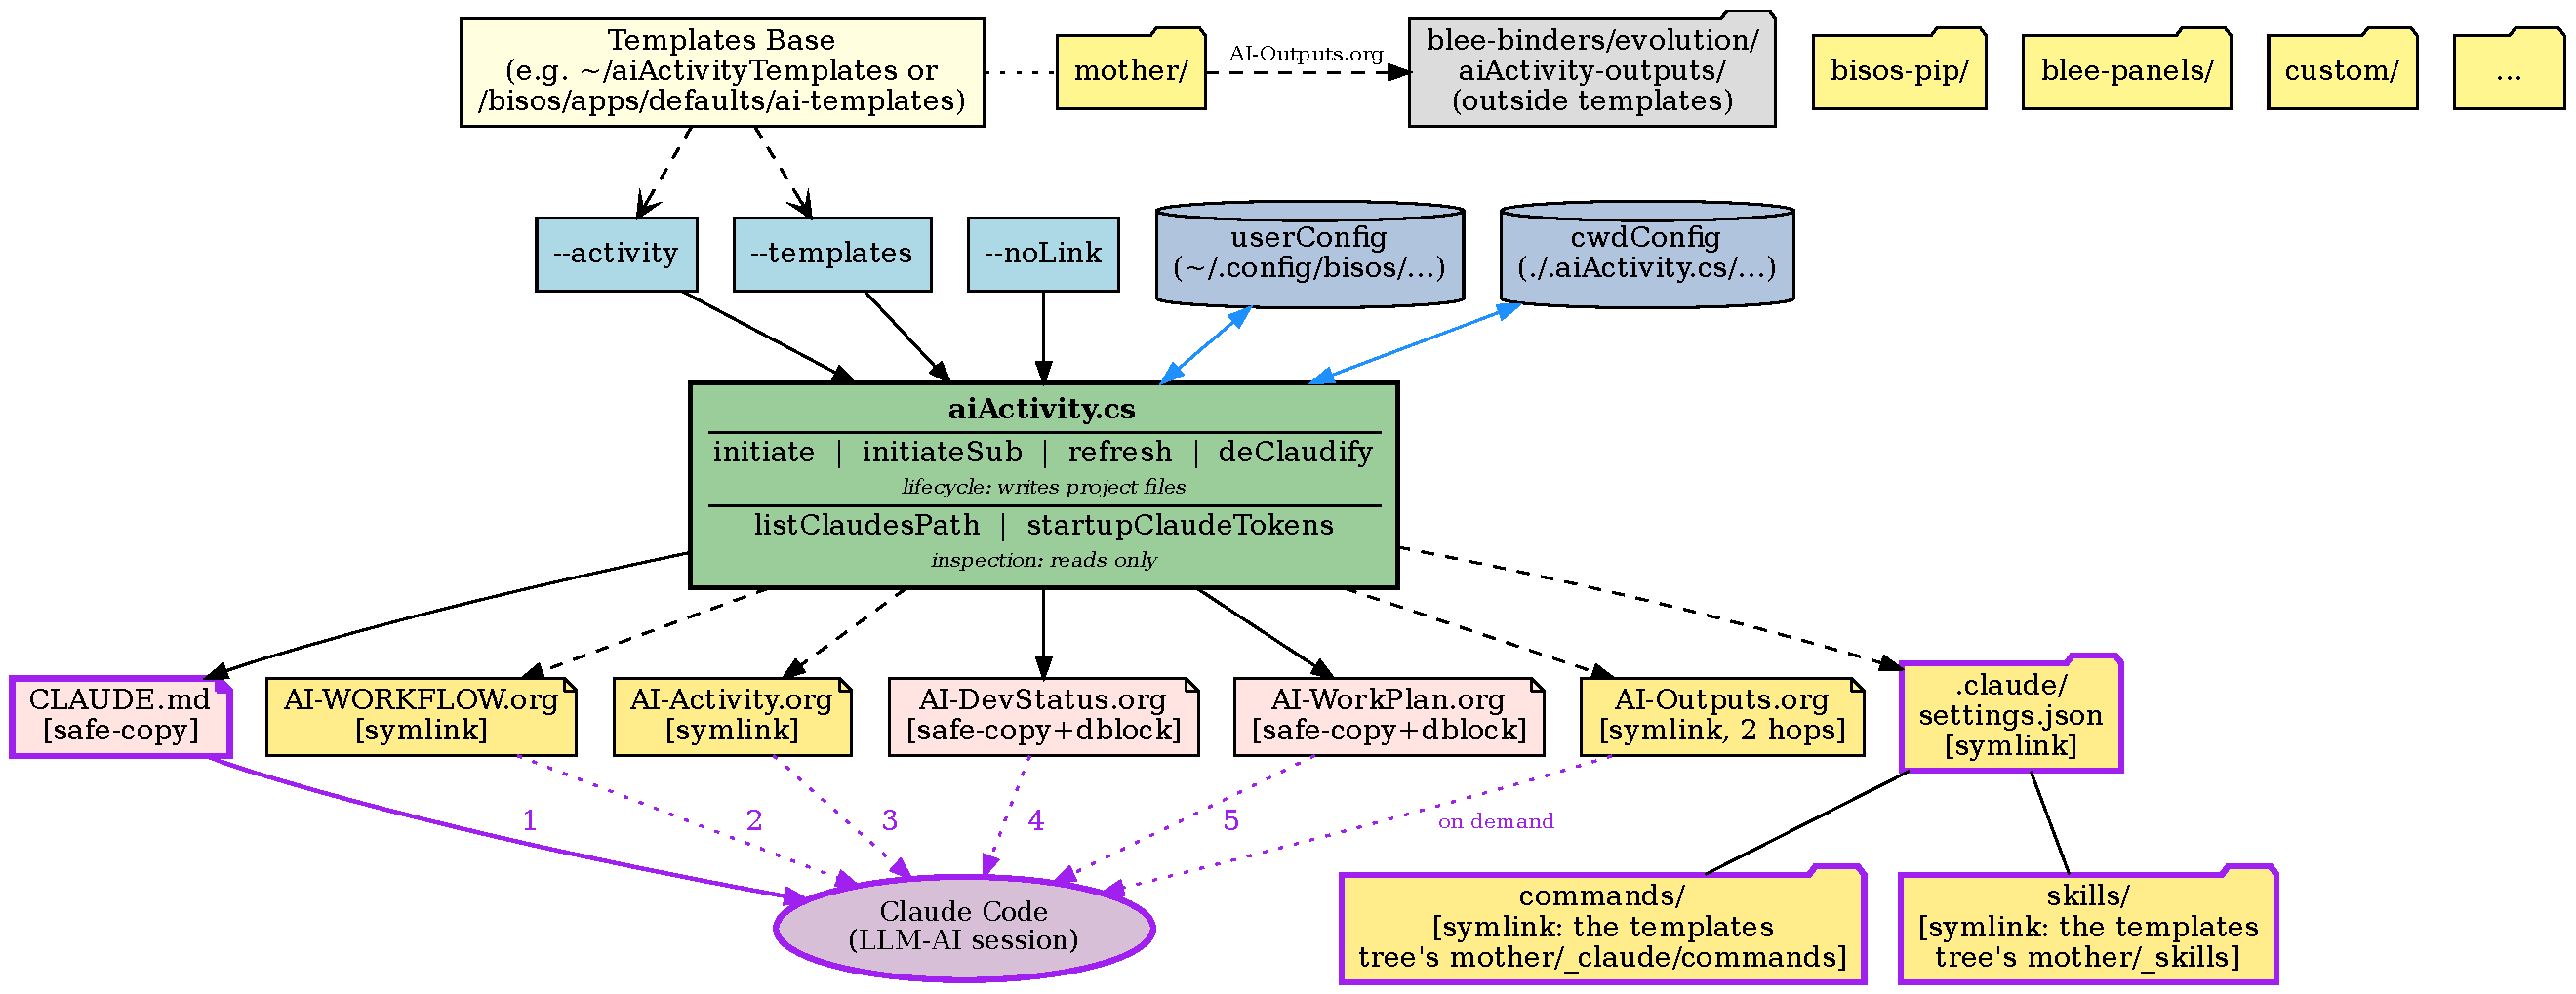
\includegraphics[width=\textwidth,height=0.95\textheight,keepaspectratio]{./figures/aiActivityFlow}
  \end{center}
\end{latexonly}
\begin{htmlonly}
  \begin{rawhtml}
<div class="center">
<img src="./figures/aiActivityFlow.png" height="450">
</div>
  \end{rawhtml}
\end{htmlonly}
\end{presentationMode}

\begin{articleMode}
  \begin{figure}[H]
    \begin{center}
      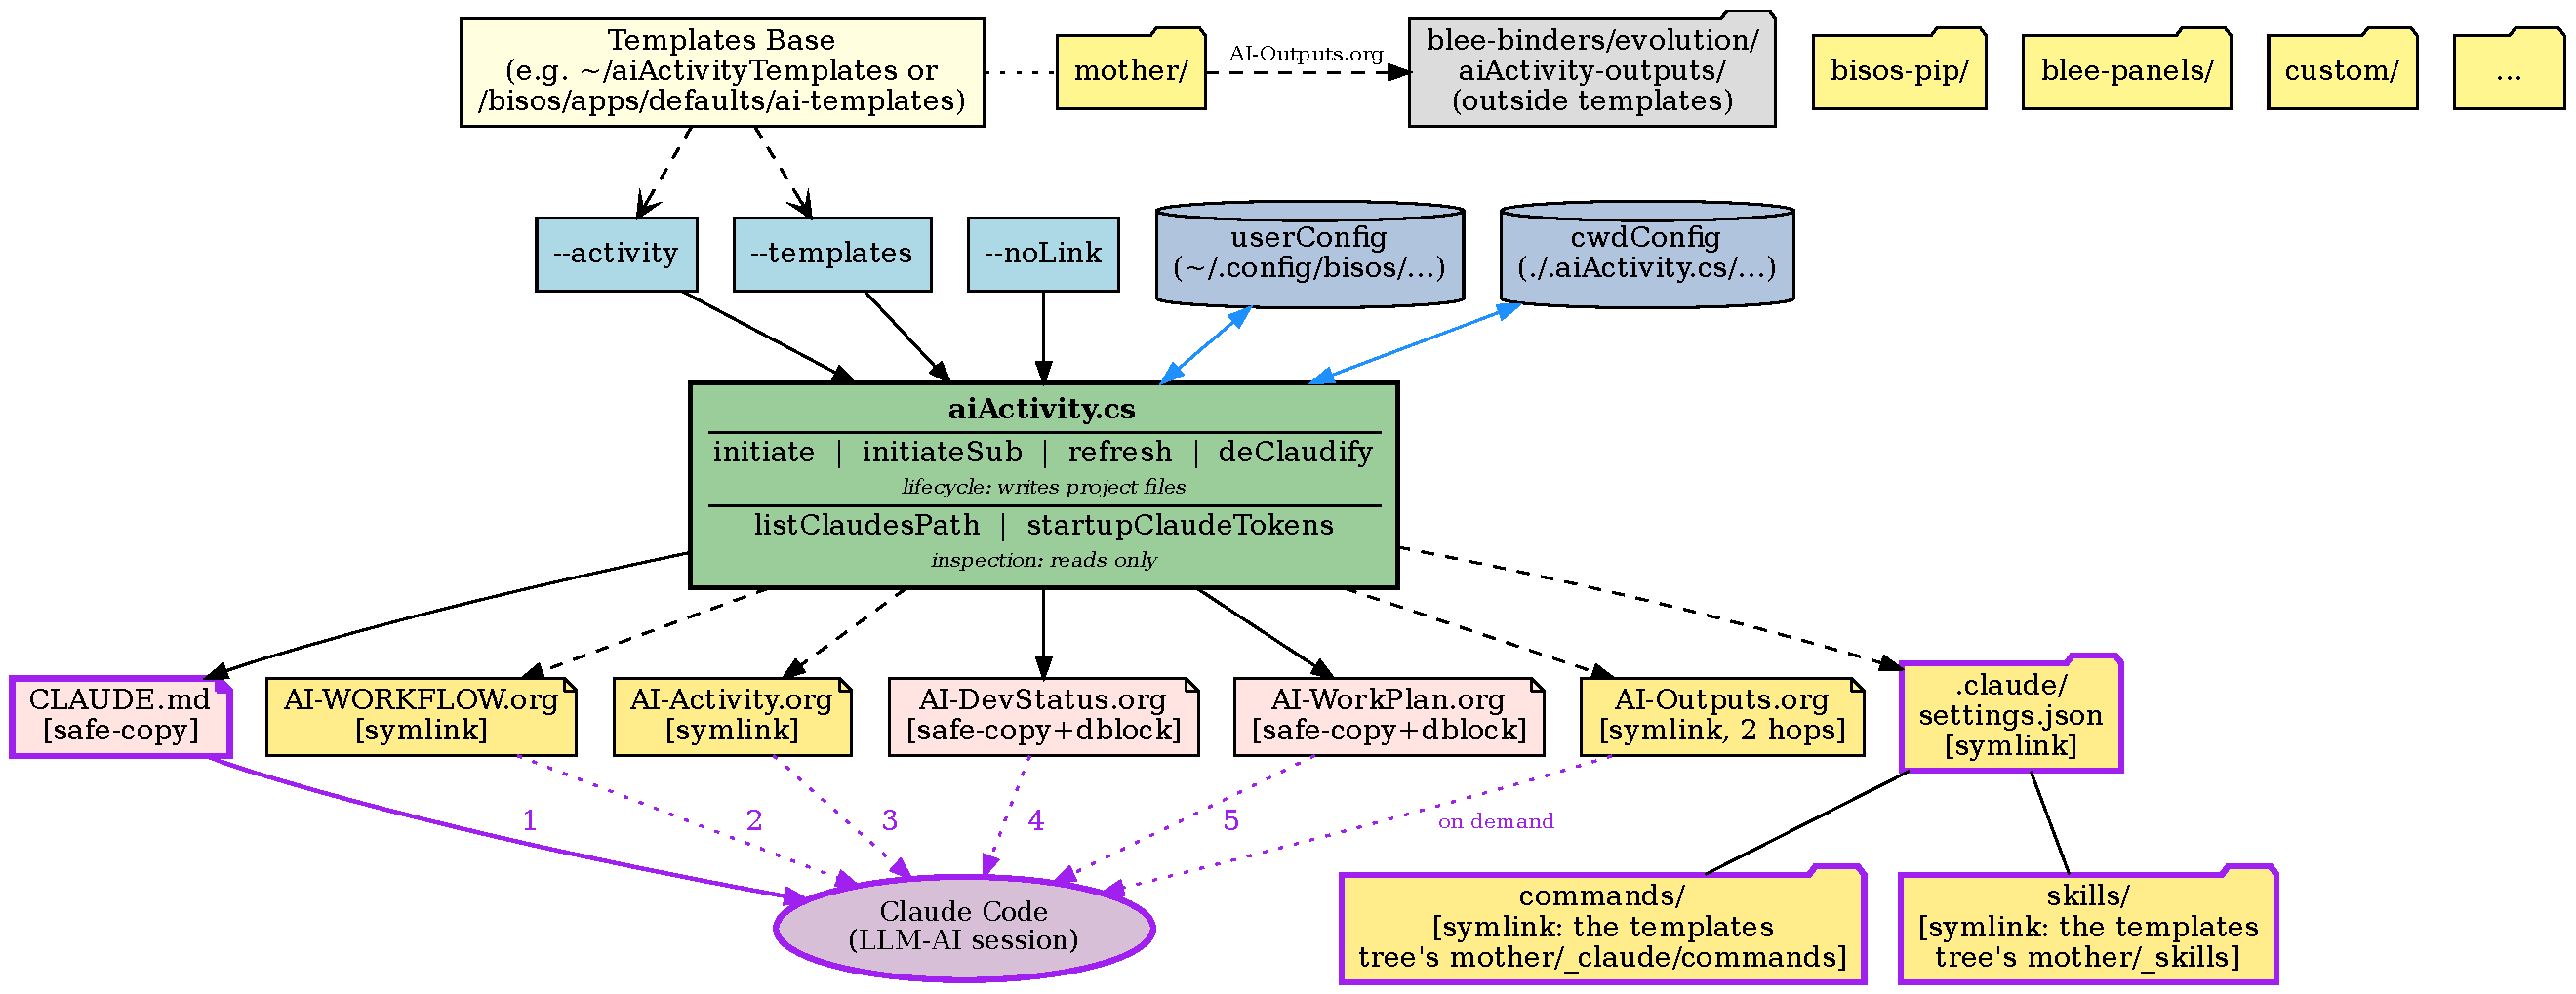
\includegraphics[width=\textwidth,height=0.8\textheight,keepaspectratio]{./figures/aiActivityFlow}
      \caption{AI-Activity Structure}
      \label{fig:aiActivityFlow}
    \end{center}
  \end{figure}
\end{articleMode}

\pnote{

This is the whole structure in one picture: the templates at the top, the engine,
the files it installs in a project, and Claude Code at the bottom, reading them at startup.
Yellow nodes are symlinks to the templates; pink nodes are per-project copies.

}

\end{frame}
\end{verblatex}



%%%#+BEGIN: bx:dblock:lcnt:latex-section :mode "auto" :seg-title "Hierarchical and Lateral AI-Activities"
%%% Args: :class "book|pres+art" :langs "en+fa" :disabledP "false" :seg-title "str" :short-title "str" :label "auto"
\begin{whenOrg}
*  _[[elisp:(blee:menu-sel:outline:popupMenu)][±]]_ _[[elisp:(blee:menu-sel:navigation:popupMenu)][Ξ]]_ [[elisp:(outline-show-branches+toggle)][|=]] [[elisp:(bx:orgm:indirectBufOther)][|>]] *[[elisp:(blee:ppmm:org-mode-toggle)][|N]]*  Section    [[elisp:(outline-show-subtree+toggle)][||]]   /Hierarchical and Lateral AI-Activities/ ::  [[elisp:(org-cycle)][| ]]
\end{whenOrg}

\section{Hierarchical and Lateral AI-Activities}
%%%#+END:

%%%#+BEGIN: b:lcnt:pres:frame/derivedImage :title "Hierarchical and Lateral AI-Activities" :subtitle "" :label "homogeneousActivity" :comment "body=figure" :reveal "plain" :beamer "plain"
\begin{whenOrg}
*****  _[[elisp:(blee:menu-sel:outline:popupMenu)][±]]_ _[[elisp:(blee:menu-sel:navigation:popupMenu)][Ξ]]_ [[elisp:(outline-show-branches+toggle)][|=]] [[elisp:(bx:orgm:indirectBufOther)][|>]] *[[elisp:(blee:ppmm:org-mode-toggle)][|N]]*  derivedImage [[elisp:(outline-show-subtree+toggle)][||]] Label=homogeneousActivity Hierarchical and Lateral AI-Activities body=figure
\end{whenOrg}

\begin{htmlonly}

\begin{frame}[fragile,plain,label=homogeneousActivity]
    \frameaudio{"audio/homogeneousActivity.mp3"}
    \frametitle{}
    \framesubtitle{}
    \begin{rawhtml}
<div class="center">
<img src="./disposition.gened/homogeneousActivity/slide-1.png" height="500">
</div>
    \end{rawhtml}
\end{frame}
\end{htmlonly}

\begin{verblatex}

\begin{frame}[fragile,plain,label=homogeneousActivity]
    \frameaudio{"audio/homogeneousActivity.mp3"}
    \frametitle{Hierarchical and Lateral AI-Activities}
    \framesubtitle{}
%%BxPy: impressiveFrameParSet('homogeneousActivity', 'always', 'True')
%%BxPy: impressiveFrameParSet('homogeneousActivity', 'transition', 'UnSpecified')
%%%#+END:

\begin{presentationMode}
\begin{latexonly}
  \vspace*{-0.25in}
  \begin{center}
    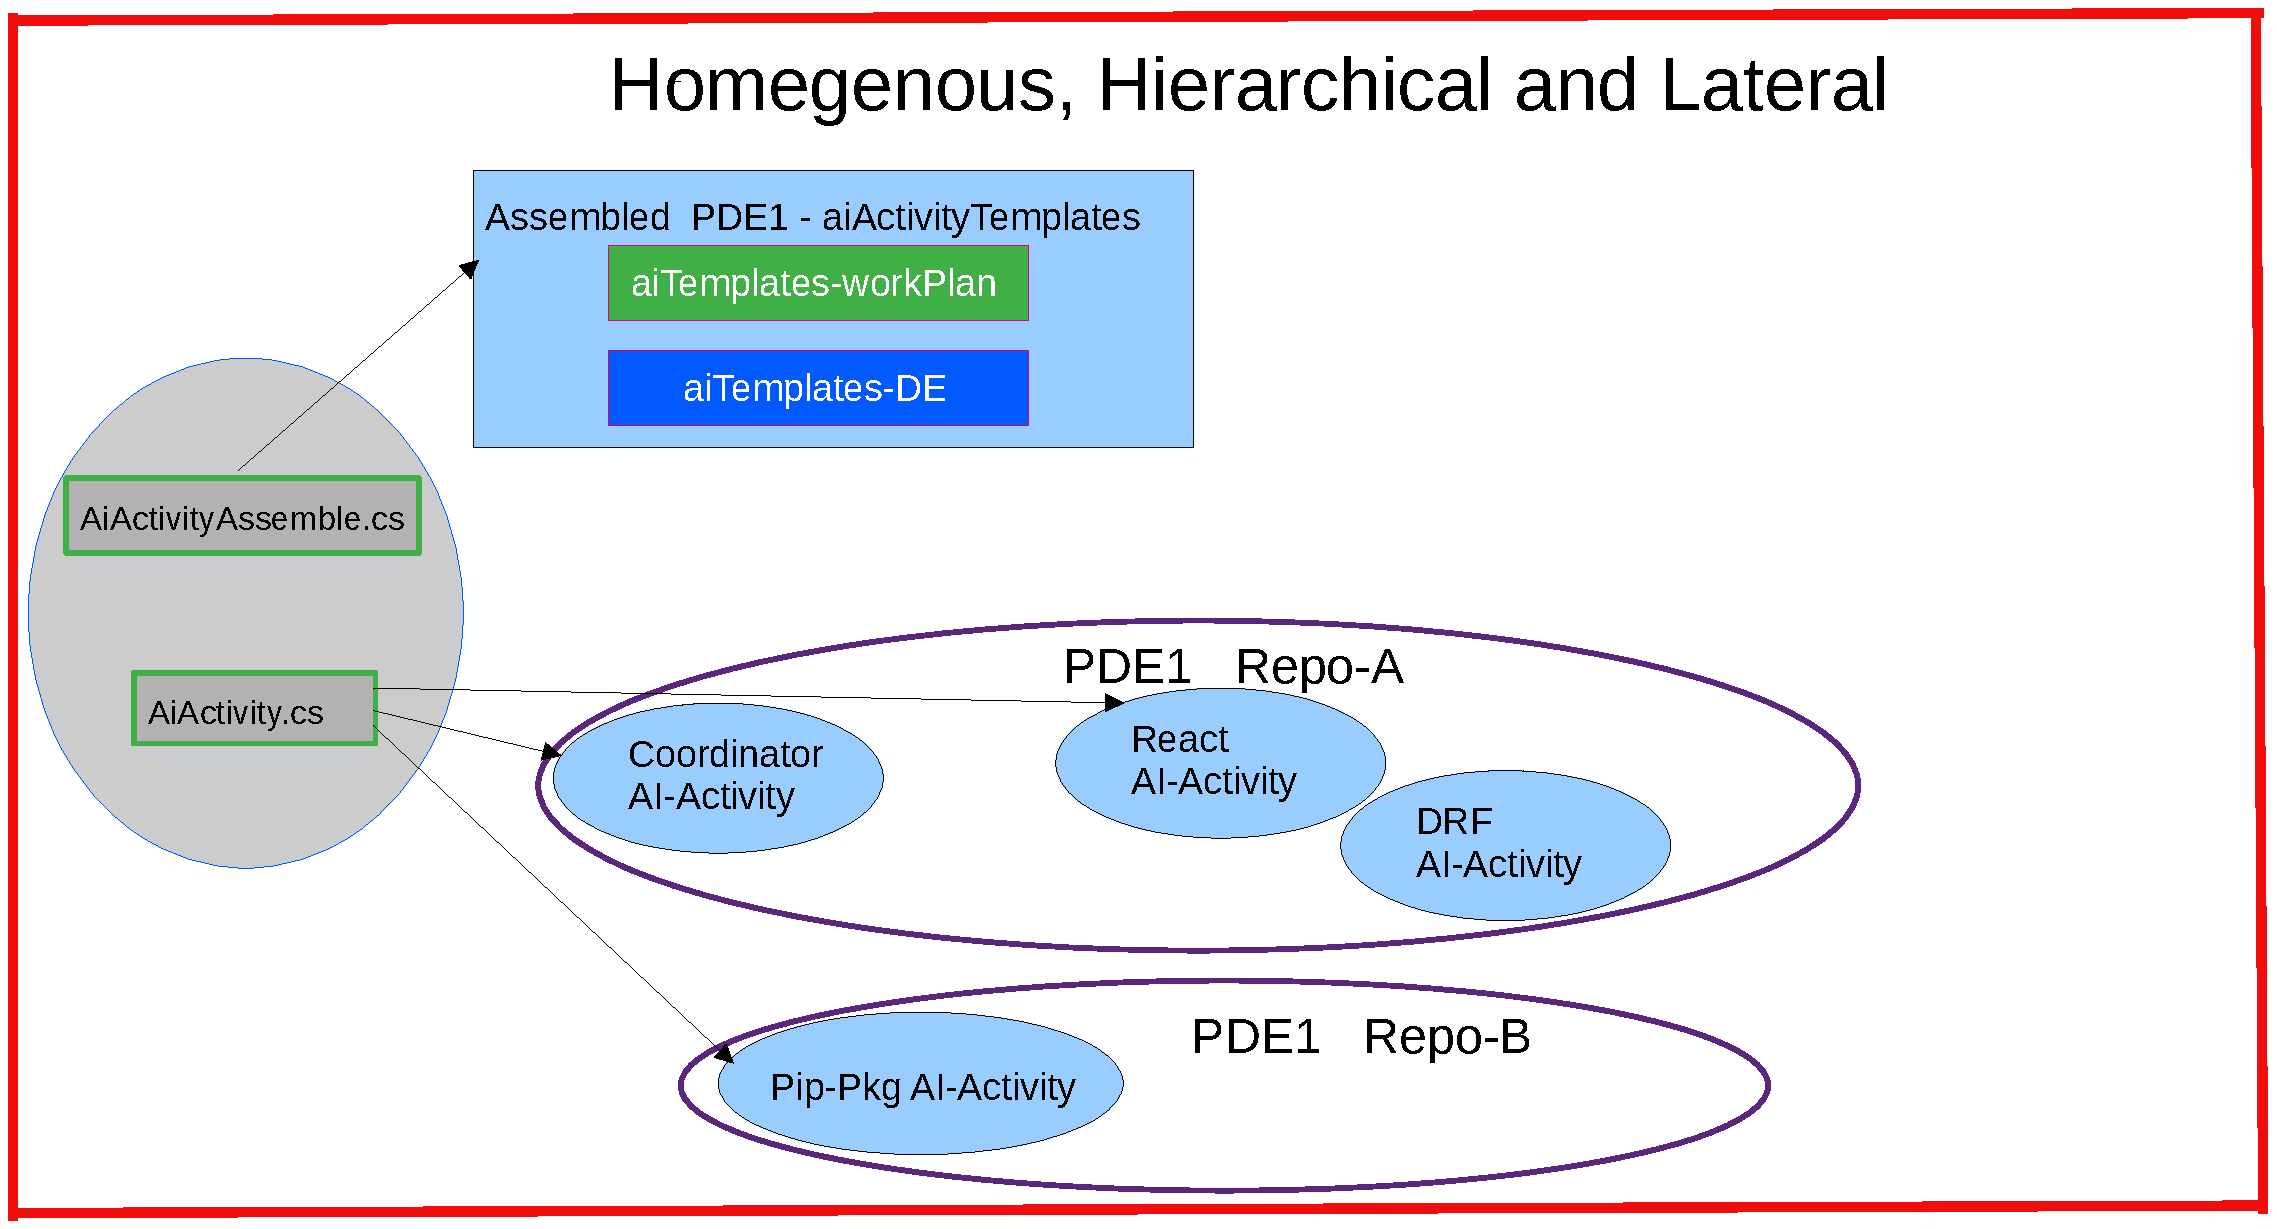
\includegraphics[width=\textwidth,height=0.95\textheight,keepaspectratio]{./figures/aiActivityHomogenous}
  \end{center}
\end{latexonly}
\begin{htmlonly}
  \begin{rawhtml}
<div class="center">
<img src="./figures/aiActivityHomogenous.png" height="450">
</div>
  \end{rawhtml}
\end{htmlonly}
\end{presentationMode}

\begin{articleMode}
  \begin{figure}[H]
    \begin{center}
      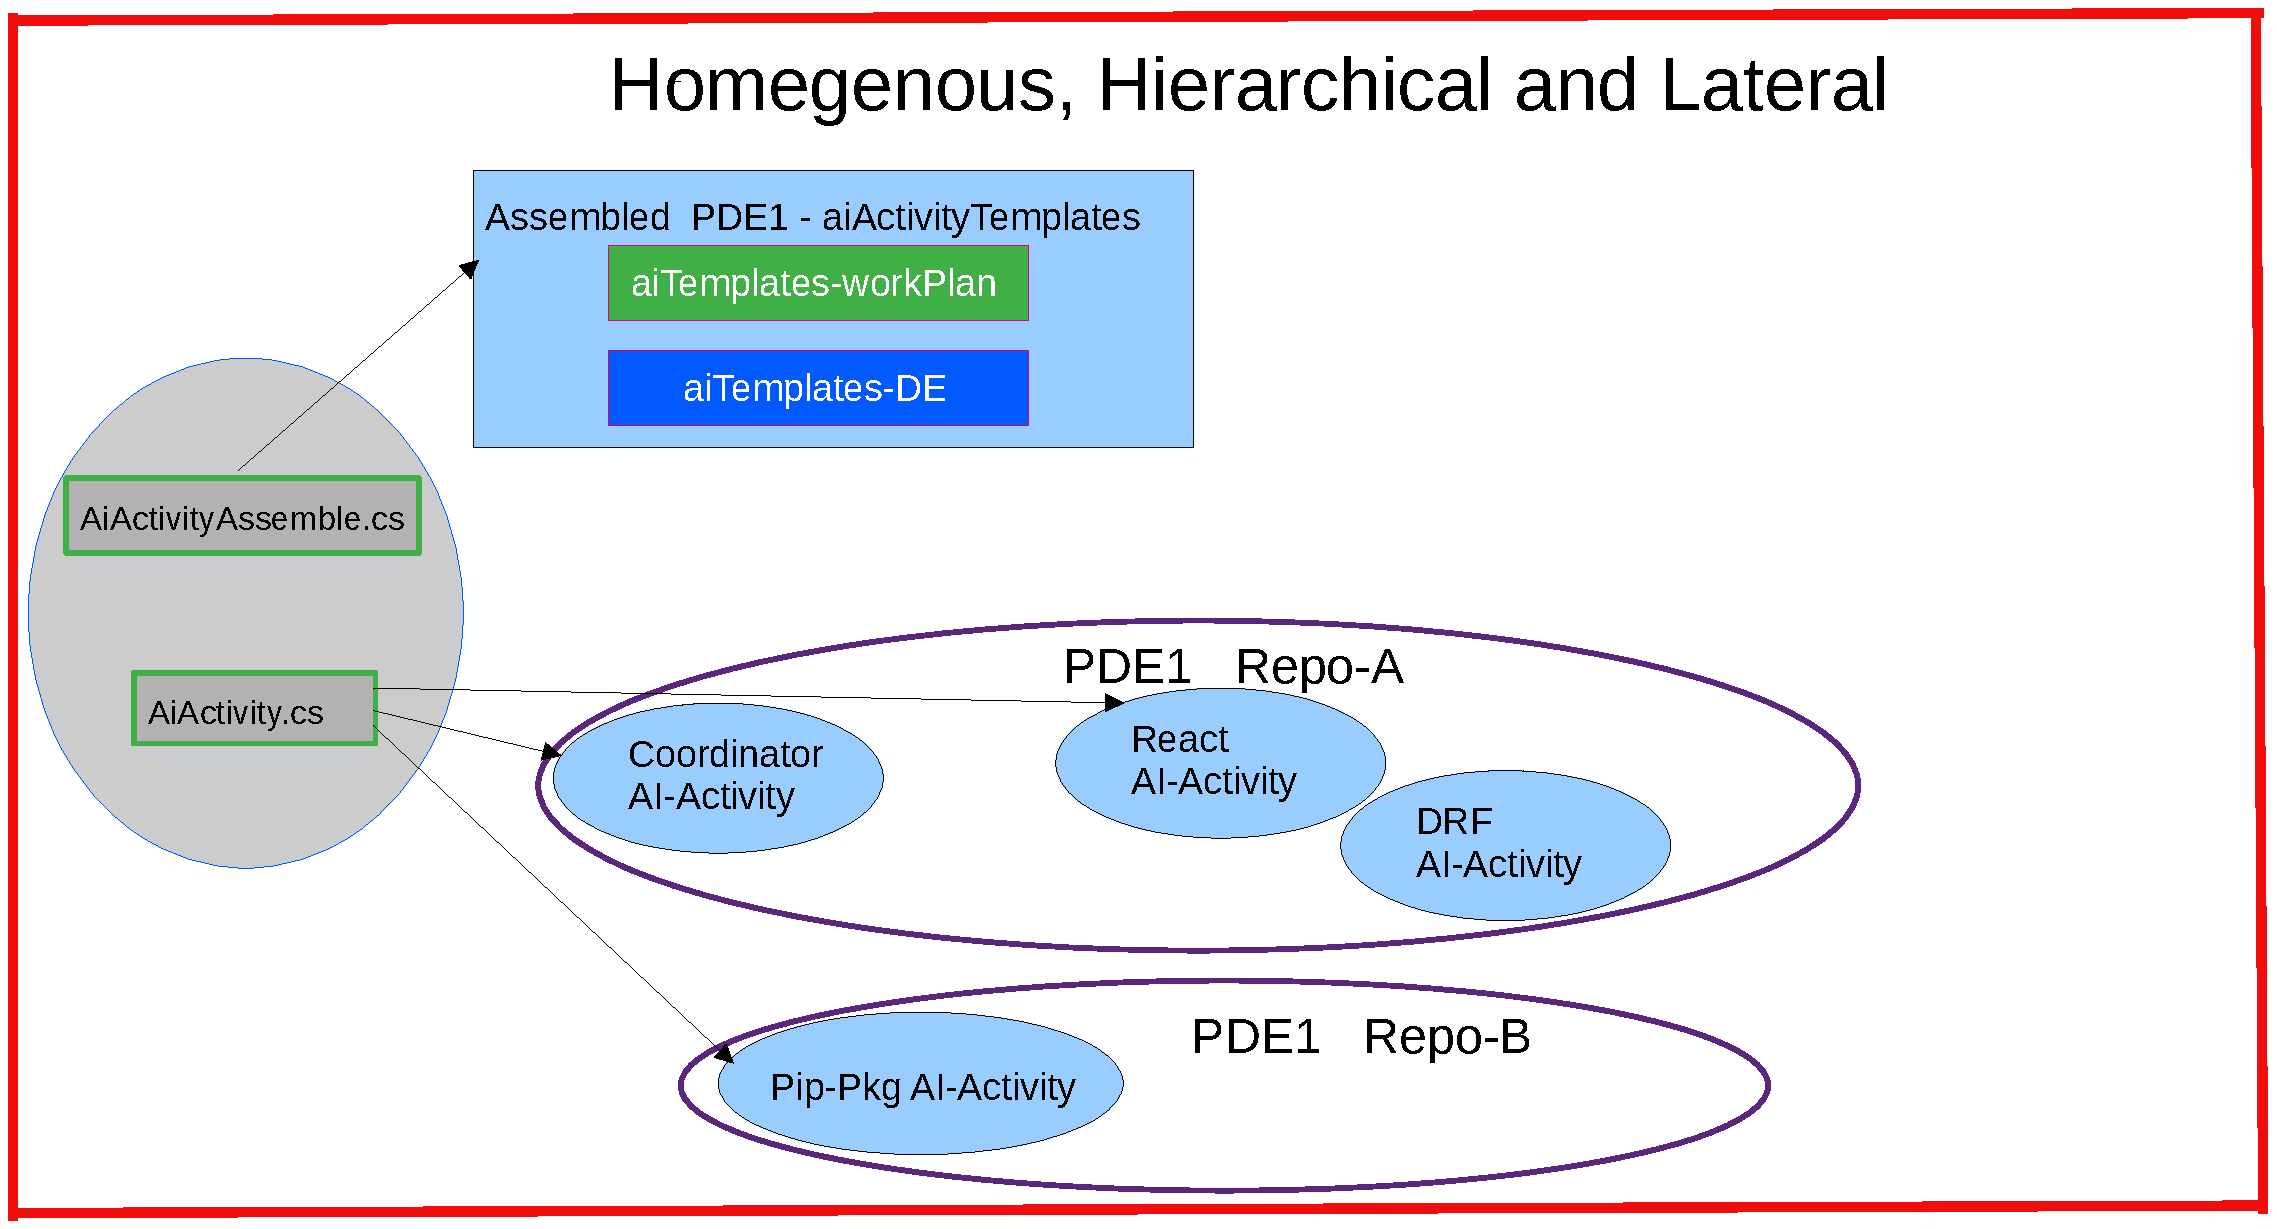
\includegraphics[width=\textwidth,height=0.8\textheight,keepaspectratio]{./figures/aiActivityHomogenous}
      \caption{Homogeneous, Hierarchical and Lateral AI-Activity}
      \label{fig:aiActivityHomogenous}
    \end{center}
  \end{figure}
\end{articleMode}

\pnote{

Projects are decomposed with a hierarchical, tree-and-siblings model.
initiate installs an AI-Activity root; initiateSub installs a slim sub inside it.
A base repo and its subprojects each carry their own plan, while inheriting shared conventions.

}

\end{frame}
\end{verblatex}



%%%#+BEGIN: b:lcnt:pres:frame/derivedImage :title "Heterogeneous AI-Activities" :subtitle "" :label "heterogeneousActivity" :comment "body=figure" :reveal "plain" :beamer "plain"
\begin{whenOrg}
*****  _[[elisp:(blee:menu-sel:outline:popupMenu)][±]]_ _[[elisp:(blee:menu-sel:navigation:popupMenu)][Ξ]]_ [[elisp:(outline-show-branches+toggle)][|=]] [[elisp:(bx:orgm:indirectBufOther)][|>]] *[[elisp:(blee:ppmm:org-mode-toggle)][|N]]*  derivedImage [[elisp:(outline-show-subtree+toggle)][||]] Label=heterogeneousActivity Heterogeneous AI-Activities body=figure
\end{whenOrg}

\begin{htmlonly}

\begin{frame}[fragile,plain,label=heterogeneousActivity]
    \frameaudio{"audio/heterogeneousActivity.mp3"}
    \frametitle{}
    \framesubtitle{}
    \begin{rawhtml}
<div class="center">
<img src="./disposition.gened/heterogeneousActivity/slide-1.png" height="500">
</div>
    \end{rawhtml}
\end{frame}
\end{htmlonly}

\begin{verblatex}

\begin{frame}[fragile,plain,label=heterogeneousActivity]
    \frameaudio{"audio/heterogeneousActivity.mp3"}
    \frametitle{Heterogeneous AI-Activities}
    \framesubtitle{}
%%BxPy: impressiveFrameParSet('heterogeneousActivity', 'always', 'True')
%%BxPy: impressiveFrameParSet('heterogeneousActivity', 'transition', 'UnSpecified')
%%%#+END:

\begin{presentationMode}
\begin{latexonly}
  \vspace*{-0.25in}
  \begin{center}
    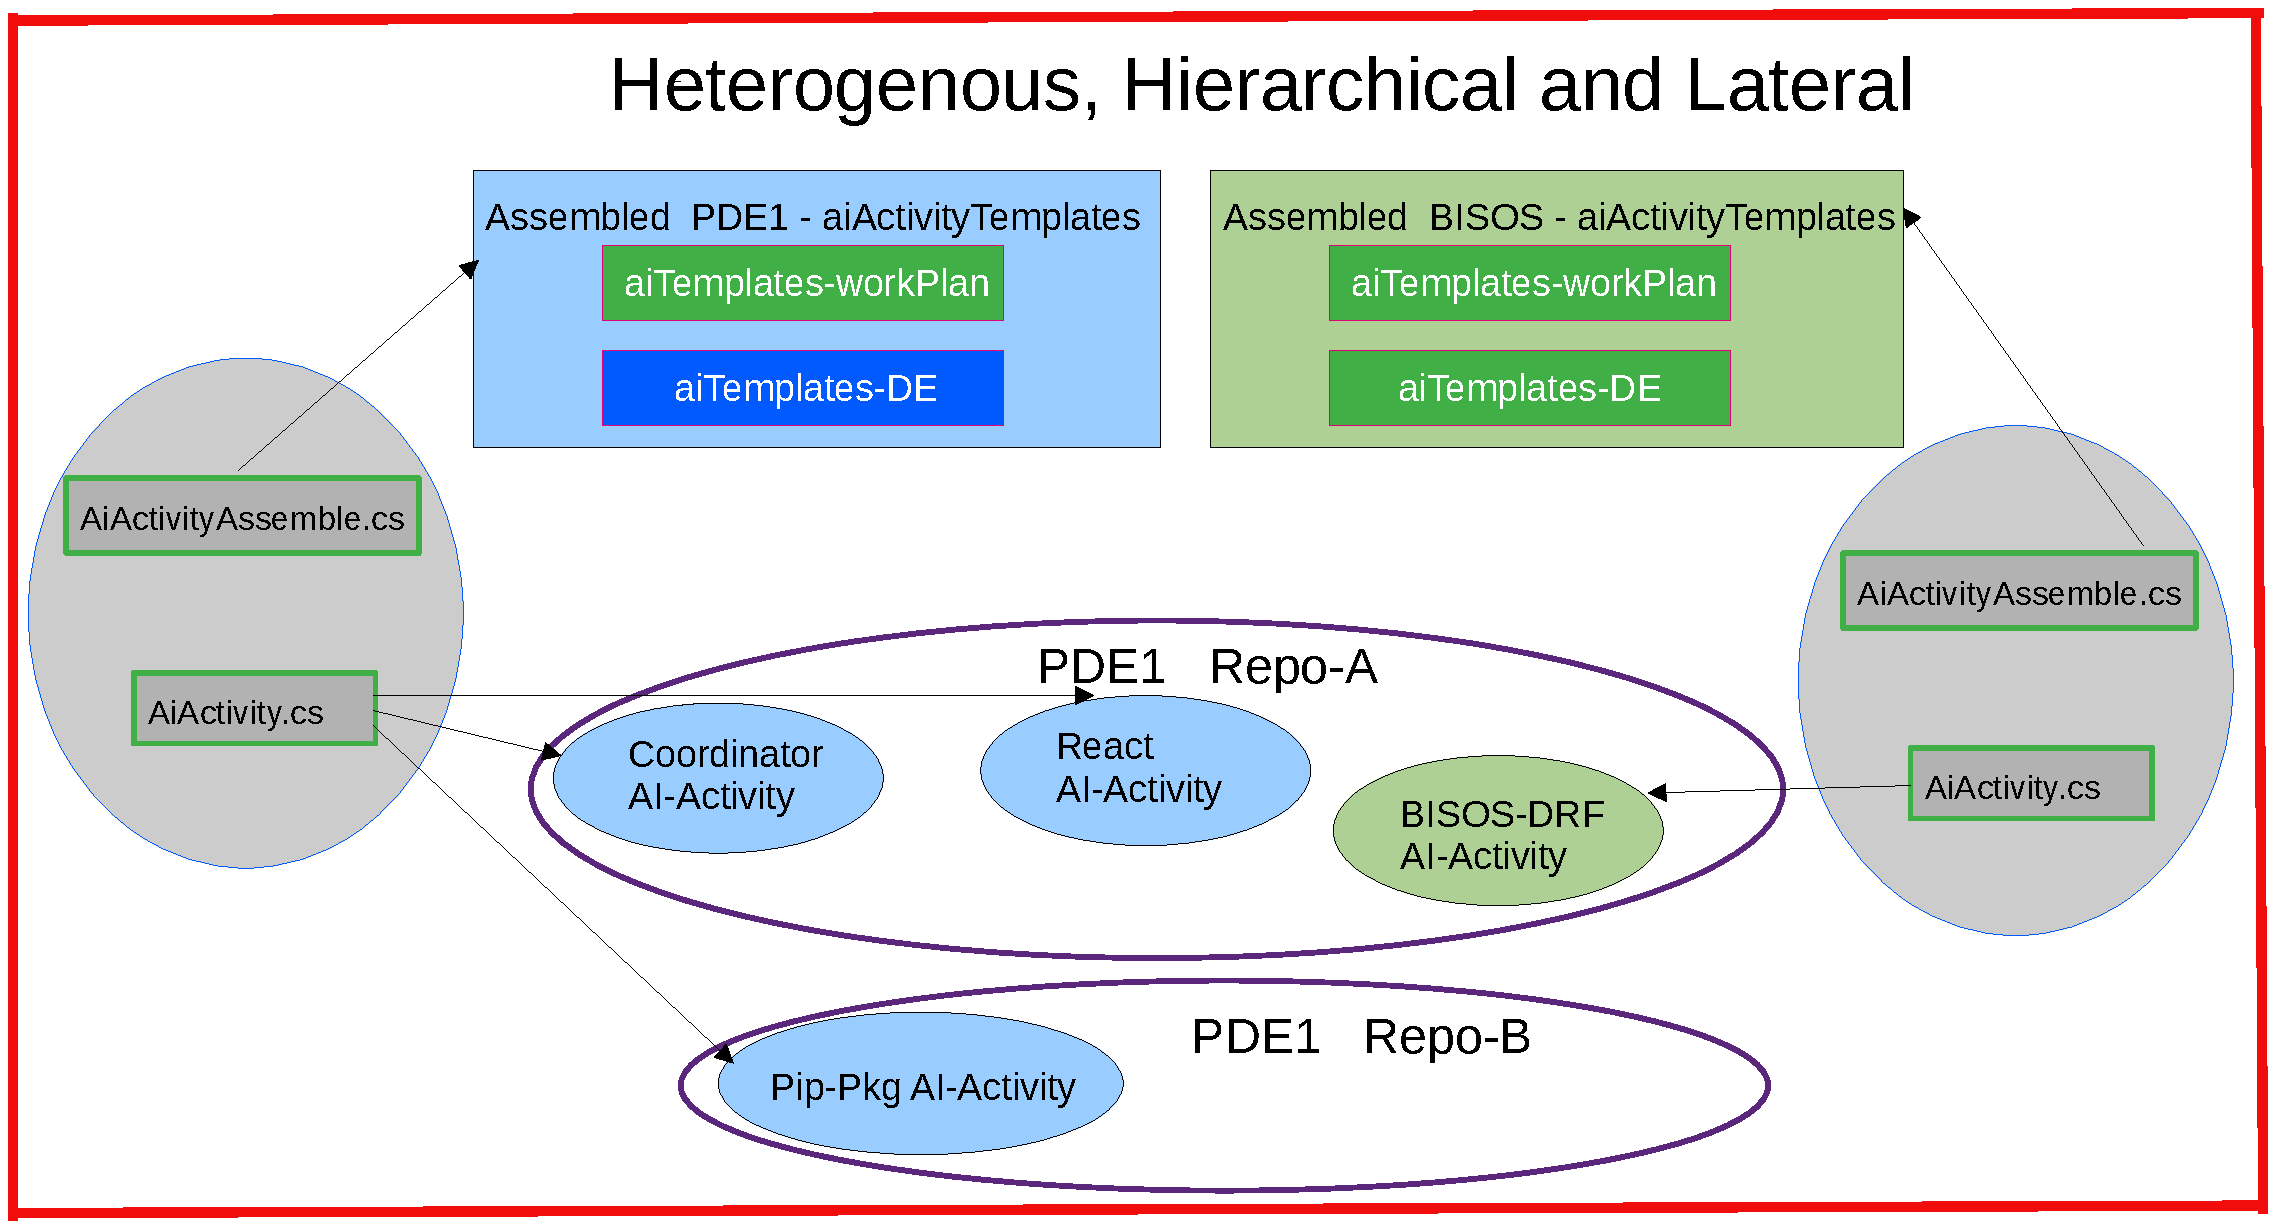
\includegraphics[width=\textwidth,height=0.95\textheight,keepaspectratio]{./figures/aiActivityHeterogenous}
  \end{center}
\end{latexonly}
\begin{htmlonly}
  \begin{rawhtml}
<div class="center">
<img src="./figures/aiActivityHeterogenous.png" height="450">
</div>
  \end{rawhtml}
\end{htmlonly}
\end{presentationMode}

\begin{articleMode}
  \begin{figure}[H]
    \begin{center}
      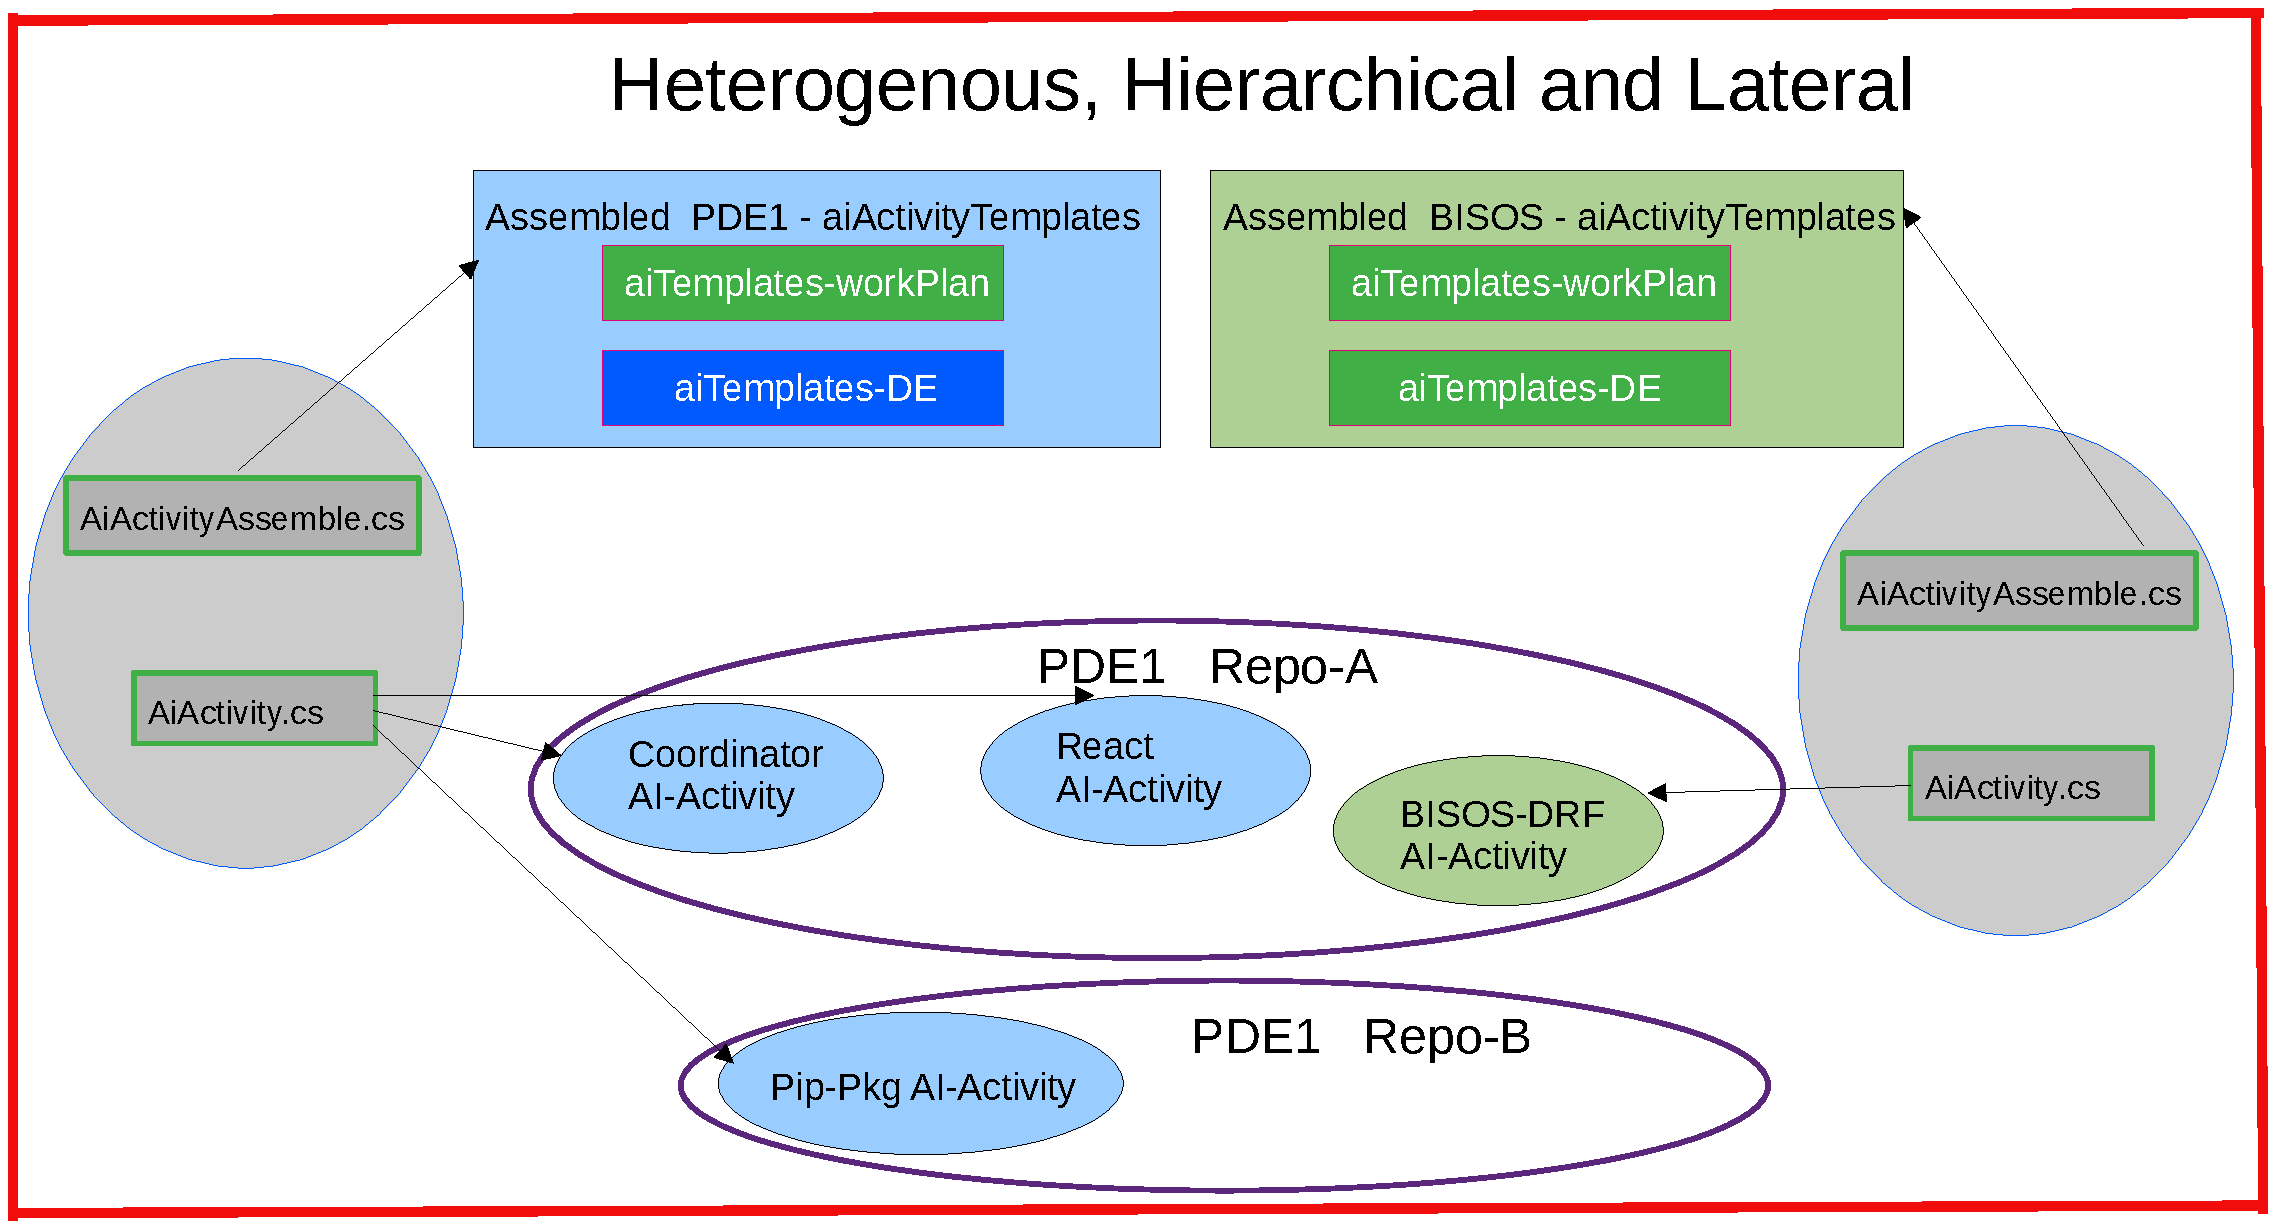
\includegraphics[width=\textwidth,height=0.8\textheight,keepaspectratio]{./figures/aiActivityHeterogenous}
      \caption{Heterogeneous, Hierarchical and Lateral AI-Activity}
      \label{fig:aiActivityHeterogenous}
    \end{center}
  \end{figure}
\end{articleMode}

\pnote{

A subproject may draw on a different templates tree from its root:
for example, an organization's own tree at the root, with a sub from the BISOS tree.
The sub then brings all of its tree's skills.

}

\end{frame}
\end{verblatex}



%%%#+BEGIN: bx:dblock:lcnt:latex-section :mode "auto" :seg-title "A Session's AI-Activities"
%%% Args: :class "book|pres+art" :langs "en+fa" :disabledP "false" :seg-title "str" :short-title "str" :label "auto"
\begin{whenOrg}
*  _[[elisp:(blee:menu-sel:outline:popupMenu)][±]]_ _[[elisp:(blee:menu-sel:navigation:popupMenu)][Ξ]]_ [[elisp:(outline-show-branches+toggle)][|=]] [[elisp:(bx:orgm:indirectBufOther)][|>]] *[[elisp:(blee:ppmm:org-mode-toggle)][|N]]*  Section    [[elisp:(outline-show-subtree+toggle)][||]]   /A Session's AI-Activities/ ::  [[elisp:(org-cycle)][| ]]
\end{whenOrg}

\section{A Session's AI-Activities}
%%%#+END:

%%%#+BEGIN: b:lcnt:pres:frame/derivedImage :title "A Session's AI-Activities: Session-Root, Native, Foreign" :subtitle "" :label "sessionActivities" :comment "body=itemize" :reveal "plain" :beamer "plain"
\begin{whenOrg}
*****  _[[elisp:(blee:menu-sel:outline:popupMenu)][±]]_ _[[elisp:(blee:menu-sel:navigation:popupMenu)][Ξ]]_ [[elisp:(outline-show-branches+toggle)][|=]] [[elisp:(bx:orgm:indirectBufOther)][|>]] *[[elisp:(blee:ppmm:org-mode-toggle)][|N]]*  derivedImage [[elisp:(outline-show-subtree+toggle)][||]] Label=sessionActivities A Session's AI-Activities: Session-Root, Native, Foreign body=itemize
\end{whenOrg}

\begin{htmlonly}

\begin{frame}[fragile,plain,label=sessionActivities]
    \frameaudio{"audio/sessionActivities.mp3"}
    \frametitle{}
    \framesubtitle{}
    \begin{rawhtml}
<div class="center">
<img src="./disposition.gened/sessionActivities/slide-1.png" height="500">
</div>
    \end{rawhtml}
\end{frame}
\end{htmlonly}

\begin{verblatex}

\begin{frame}[fragile,plain,label=sessionActivities]
    \frameaudio{"audio/sessionActivities.mp3"}
    \frametitle{A Session's AI-Activities: Session-Root, Native, Foreign}
    \framesubtitle{}
%%BxPy: impressiveFrameParSet('sessionActivities', 'always', 'True')
%%BxPy: impressiveFrameParSet('sessionActivities', 'transition', 'UnSpecified')
%%%#+END:

\begin{itemize}
  \item A session is anchored at its \textbf{Session-Root} --- an AI-Activity Root
    \begin{itemize}
    \item The Session-Root decides the tooling: commands, skills, settings
    \item The AI-Activity decides the content: the \texttt{CLAUDE.md} chain
    \end{itemize}
  \item It may \textbf{reach} other AI-Activities --- \texttt{/bx-activity-reach}
    \begin{itemize}
    \item \textbf{Native}: under the Session-Root
    \item \textbf{Foreign}: under another root
    \end{itemize}
  \item This presentation: reached as a foreign AI-Activity\\
    from a session rooted in a Python package
  \end{itemize}

\pnote{

A session is anchored at its Session-Root, which decides the tooling.
The AI-Activity decides the content.

A session may reach other AI-Activities, native ones under its root and foreign ones
under other roots. In fact, this presentation was started from a session rooted in
a Python package, reaching this presentation as a foreign AI-Activity.

}

\end{frame}
\end{verblatex}



%%%#+BEGIN: bx:dblock:lcnt:latex-part :disabledP "false" :seg-title "A Walk Through the Design and Implementation"
%%% Args: :toc "NU" :tocDepth 3 :part "NU" :label "auto|spec" :partpage t
\begin{whenOrg}
*      ================
*  [[elisp:(blee:ppmm:org-mode-toggle)][|n]] [[elisp:(blee:menu-sel:outline:popupMenu)][+-]] [[elisp:(blee:menu-sel:navigation:popupMenu)][==]]  *Part*   _A Walk Through the Design and Implementation_ ::  [[elisp:(org-cycle)][| ]]
\end{whenOrg}

\newpage
\part{A Walk Through the Design and Implementation}
%%%#+END:

%%%#+BEGIN: bx:dblock:lcnt:latex-section :mode "auto" :seg-title "Setting Up an AI-Activity"
%%% Args: :class "book|pres+art" :langs "en+fa" :disabledP "false" :seg-title "str" :short-title "str" :label "auto"
\begin{whenOrg}
*  _[[elisp:(blee:menu-sel:outline:popupMenu)][±]]_ _[[elisp:(blee:menu-sel:navigation:popupMenu)][Ξ]]_ [[elisp:(outline-show-branches+toggle)][|=]] [[elisp:(bx:orgm:indirectBufOther)][|>]] *[[elisp:(blee:ppmm:org-mode-toggle)][|N]]*  Section    [[elisp:(outline-show-subtree+toggle)][||]]   /Setting Up an AI-Activity/ ::  [[elisp:(org-cycle)][| ]]
\end{whenOrg}

\section{Setting Up an AI-Activity}
%%%#+END:

%%%#+BEGIN: b:lcnt:pres:frame/derivedImage :title "Setting Up an AI-Activity" :subtitle "" :label "startupWorkflow" :comment "body=figure" :reveal "plain" :beamer "plain"
\begin{whenOrg}
*****  _[[elisp:(blee:menu-sel:outline:popupMenu)][±]]_ _[[elisp:(blee:menu-sel:navigation:popupMenu)][Ξ]]_ [[elisp:(outline-show-branches+toggle)][|=]] [[elisp:(bx:orgm:indirectBufOther)][|>]] *[[elisp:(blee:ppmm:org-mode-toggle)][|N]]*  derivedImage [[elisp:(outline-show-subtree+toggle)][||]] Label=startupWorkflow Setting Up an AI-Activity body=figure
\end{whenOrg}

\begin{htmlonly}

\begin{frame}[fragile,plain,label=startupWorkflow]
    \frameaudio{"audio/startupWorkflow.mp3"}
    \frametitle{}
    \framesubtitle{}
    \begin{rawhtml}
<div class="center">
<img src="./disposition.gened/startupWorkflow/slide-1.png" height="500">
</div>
    \end{rawhtml}
\end{frame}
\end{htmlonly}

\begin{verblatex}

\begin{frame}[fragile,plain,label=startupWorkflow]
    \frameaudio{"audio/startupWorkflow.mp3"}
    \frametitle{Setting Up an AI-Activity}
    \framesubtitle{}
%%BxPy: impressiveFrameParSet('startupWorkflow', 'always', 'True')
%%BxPy: impressiveFrameParSet('startupWorkflow', 'transition', 'UnSpecified')
%%%#+END:

\begin{presentationMode}
\begin{latexonly}
  \vspace*{-0.25in}
  \begin{center}
    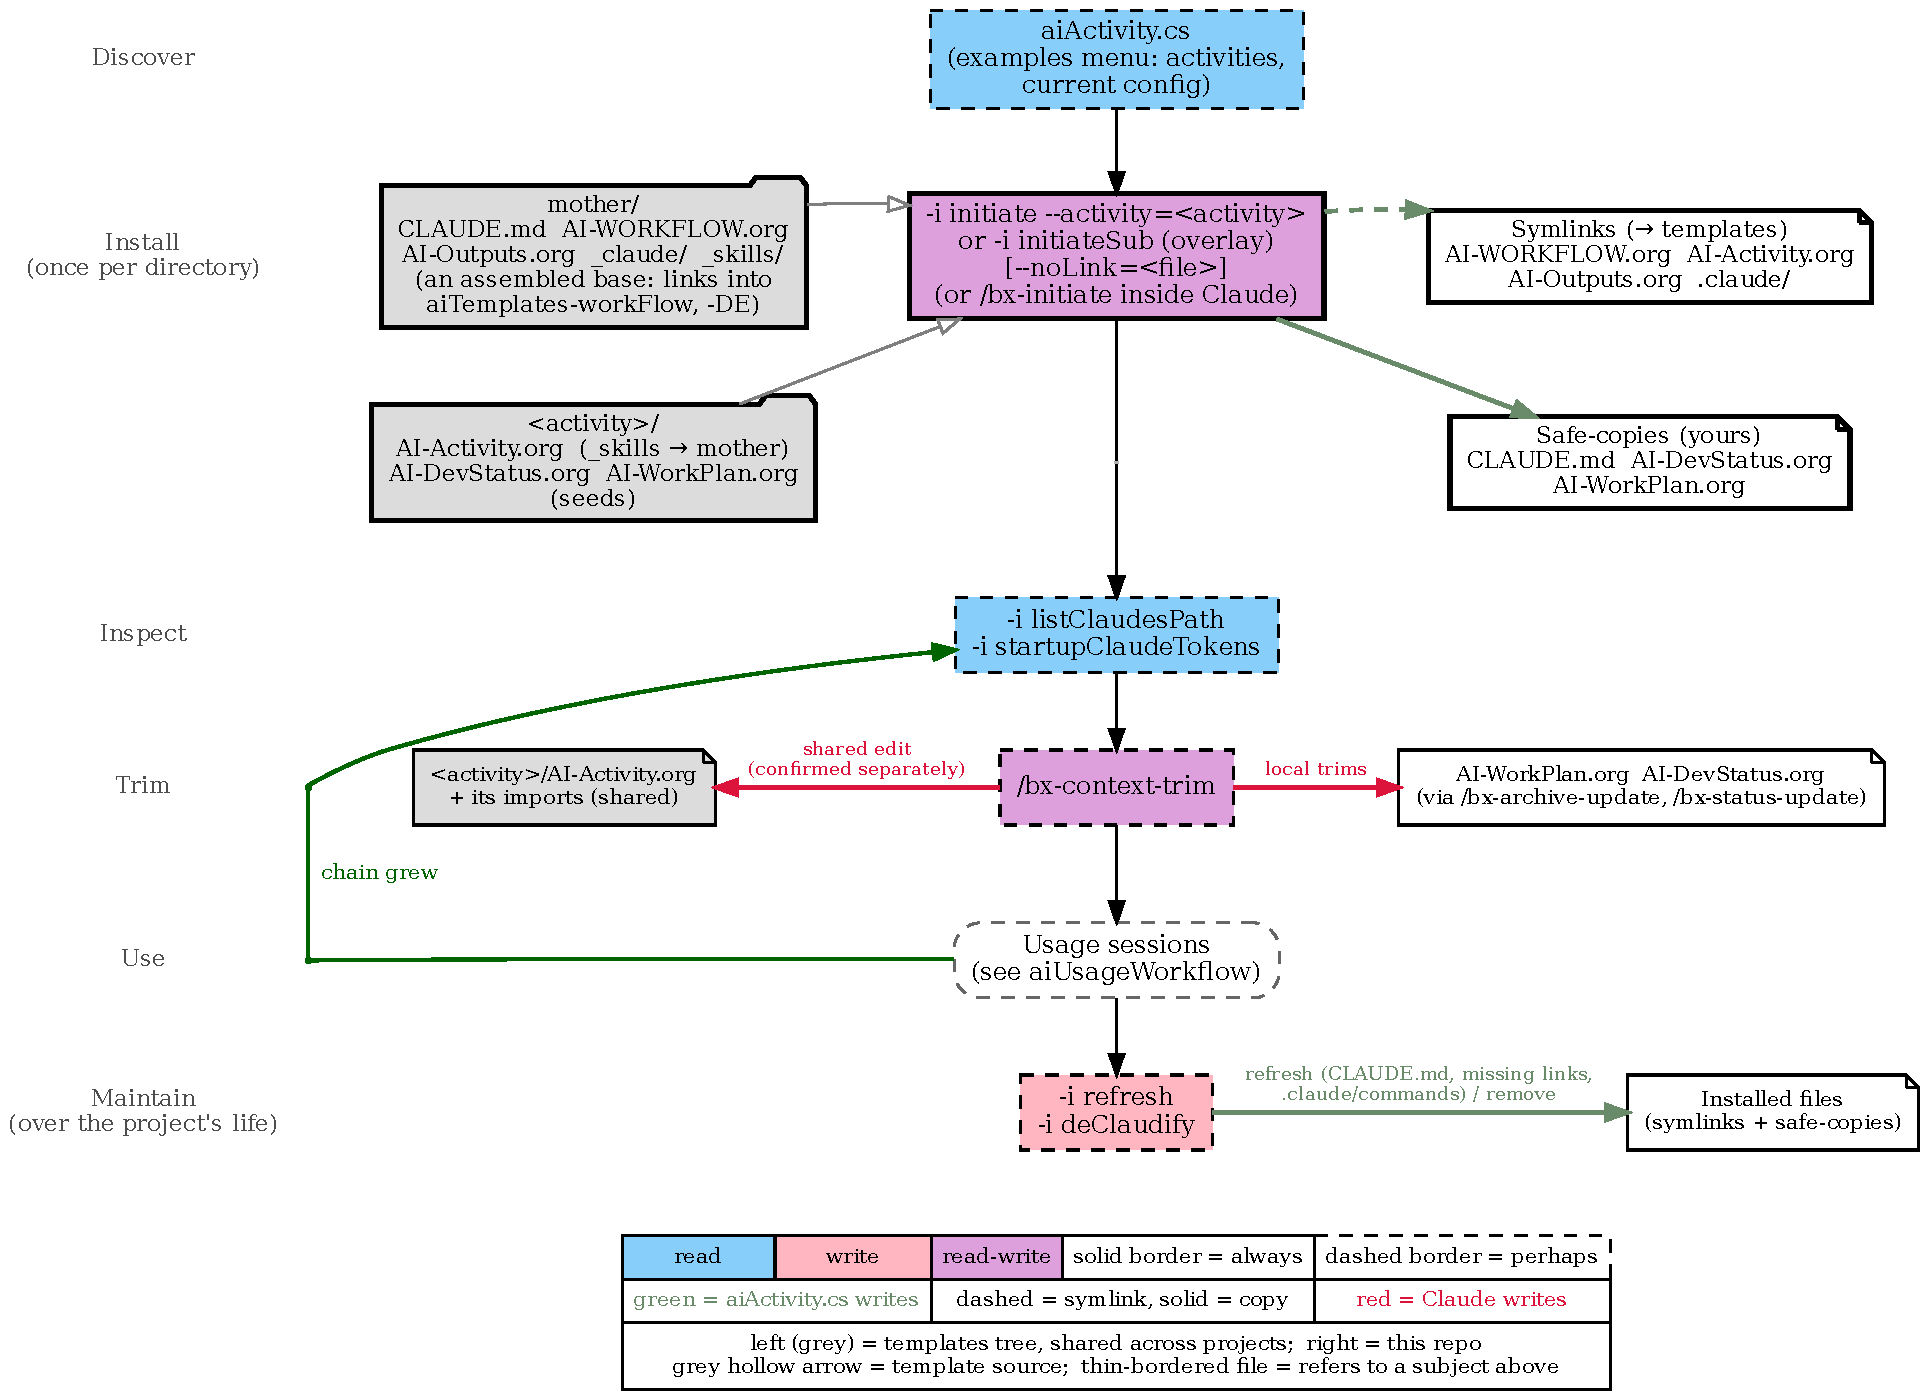
\includegraphics[width=\textwidth,height=0.95\textheight,keepaspectratio]{./figures/aiStartupWorkflow}
  \end{center}
\end{latexonly}
\begin{htmlonly}
  \begin{rawhtml}
<div class="center">
<img src="./figures/aiStartupWorkflow.png" height="450">
</div>
  \end{rawhtml}
\end{htmlonly}
\end{presentationMode}

\begin{articleMode}
  \begin{figure}[H]
    \begin{center}
      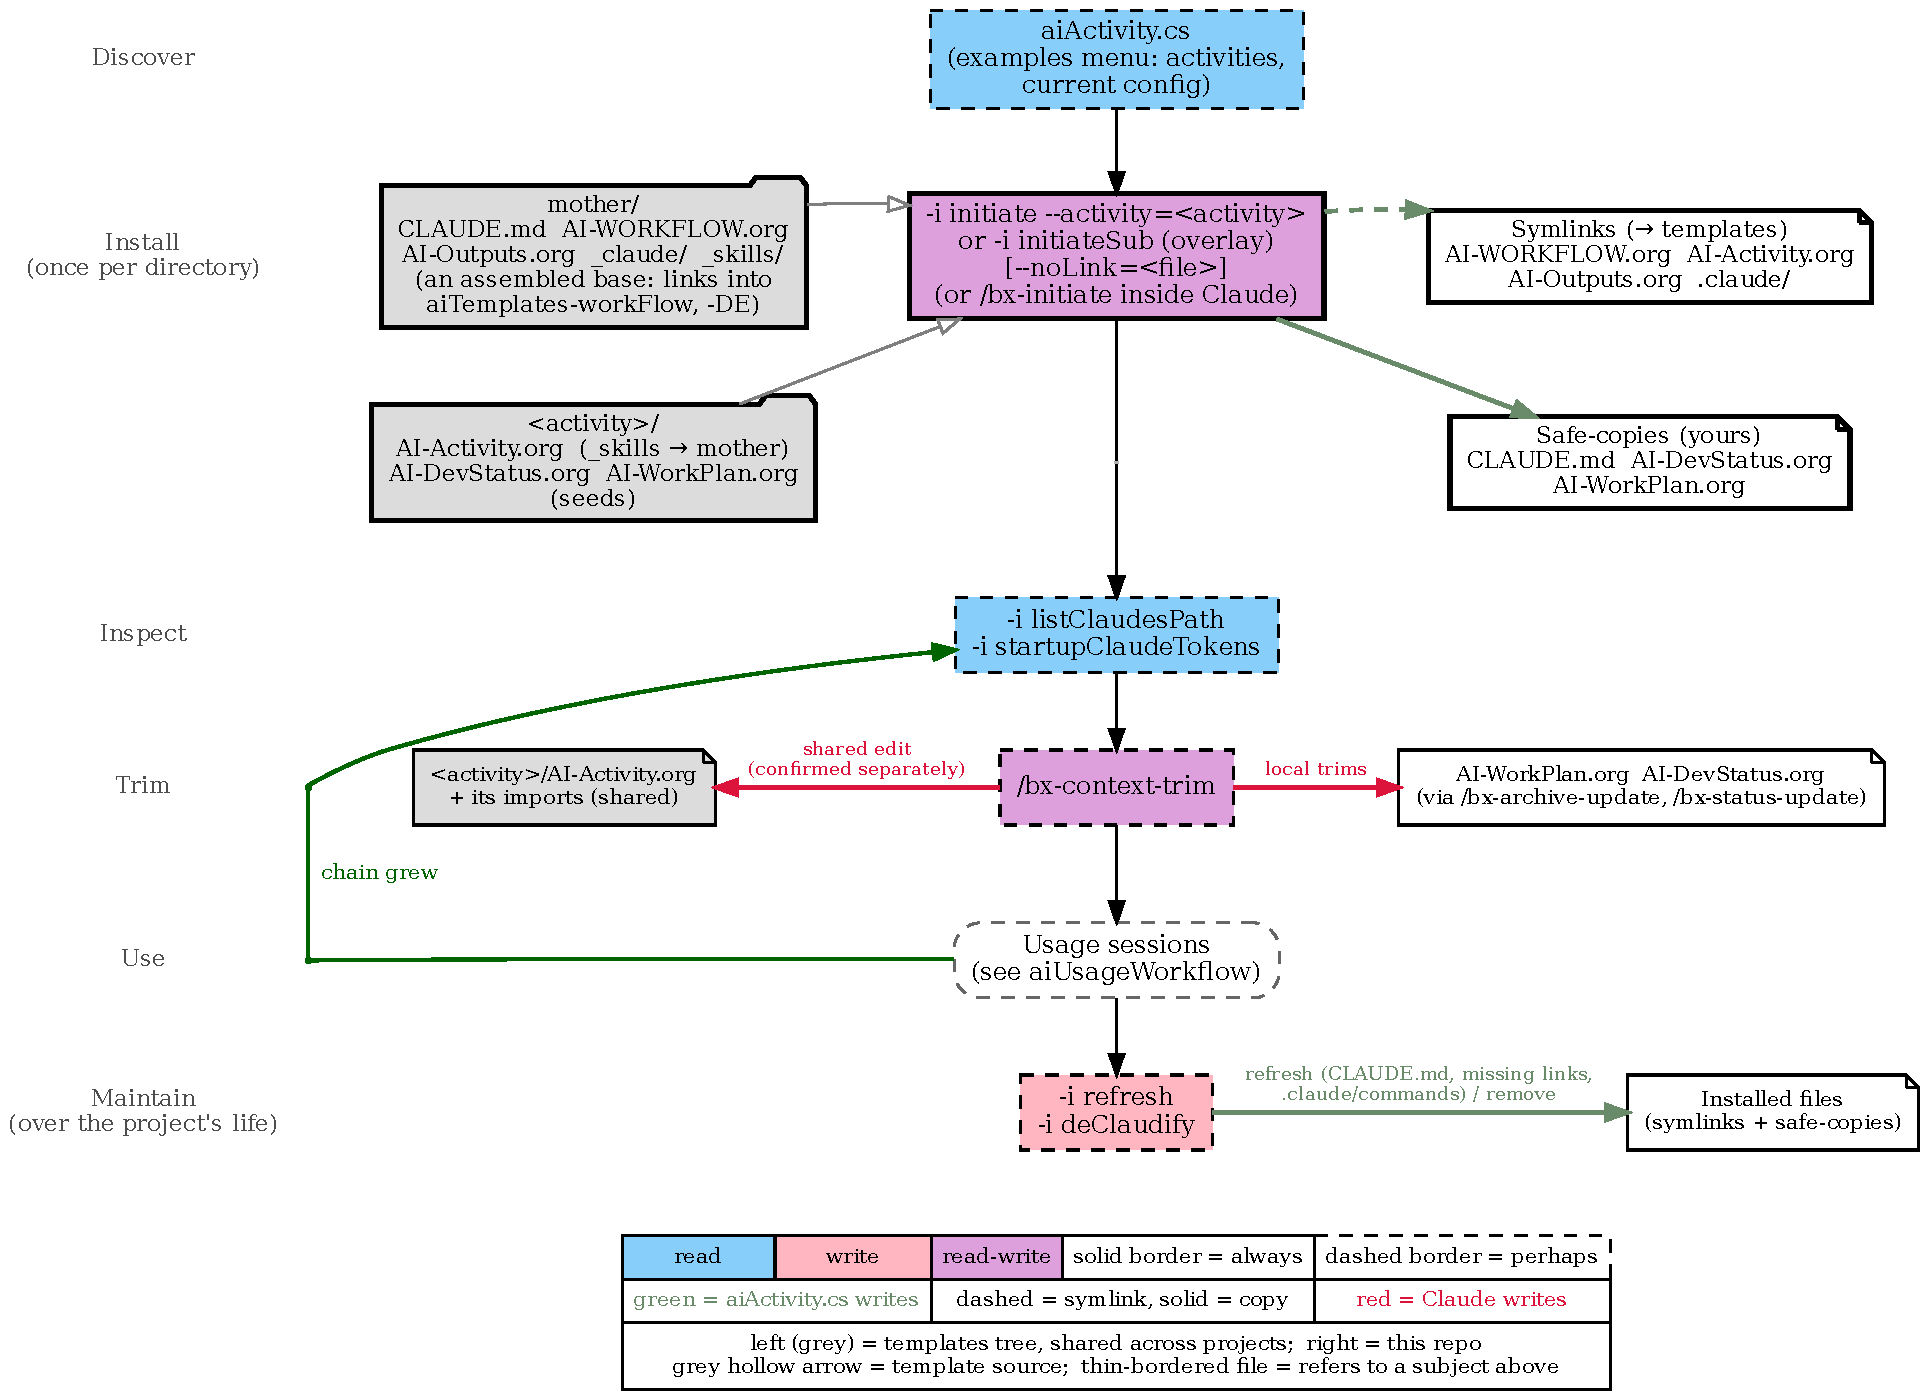
\includegraphics[width=\textwidth,height=0.8\textheight,keepaspectratio]{./figures/aiStartupWorkflow}
      \caption{AI-Activity Startup Workflow}
      \label{fig:aiStartupWorkflow}
    \end{center}
  \end{figure}
\end{articleMode}

\pnote{

This is how an AI-Activity setup comes into being: discover the activities,
install from the shared templates into the repository, inspect and trim the startup context,
use it, and maintain it.

}

\end{frame}
\end{verblatex}



%%%#+BEGIN: bx:dblock:lcnt:latex-section :mode "auto" :seg-title "A Session, Command by Command"
%%% Args: :class "book|pres+art" :langs "en+fa" :disabledP "false" :seg-title "str" :short-title "str" :label "auto"
\begin{whenOrg}
*  _[[elisp:(blee:menu-sel:outline:popupMenu)][±]]_ _[[elisp:(blee:menu-sel:navigation:popupMenu)][Ξ]]_ [[elisp:(outline-show-branches+toggle)][|=]] [[elisp:(bx:orgm:indirectBufOther)][|>]] *[[elisp:(blee:ppmm:org-mode-toggle)][|N]]*  Section    [[elisp:(outline-show-subtree+toggle)][||]]   /A Session, Command by Command/ ::  [[elisp:(org-cycle)][| ]]
\end{whenOrg}

\section{A Session, Command by Command}
%%%#+END:

%%%#+BEGIN: b:lcnt:pres:frame/derivedImage :title "A Session, Command by Command" :subtitle "" :label "usageWorkflow" :comment "body=figure" :reveal "plain" :beamer "plain"
\begin{whenOrg}
*****  _[[elisp:(blee:menu-sel:outline:popupMenu)][±]]_ _[[elisp:(blee:menu-sel:navigation:popupMenu)][Ξ]]_ [[elisp:(outline-show-branches+toggle)][|=]] [[elisp:(bx:orgm:indirectBufOther)][|>]] *[[elisp:(blee:ppmm:org-mode-toggle)][|N]]*  derivedImage [[elisp:(outline-show-subtree+toggle)][||]] Label=usageWorkflow A Session, Command by Command body=figure
\end{whenOrg}

\begin{htmlonly}

\begin{frame}[fragile,plain,label=usageWorkflow]
    \frameaudio{"audio/usageWorkflow.mp3"}
    \frametitle{}
    \framesubtitle{}
    \begin{rawhtml}
<div class="center">
<img src="./disposition.gened/usageWorkflow/slide-1.png" height="500">
</div>
    \end{rawhtml}
\end{frame}
\end{htmlonly}

\begin{verblatex}

\begin{frame}[fragile,plain,label=usageWorkflow]
    \frameaudio{"audio/usageWorkflow.mp3"}
    \frametitle{A Session, Command by Command}
    \framesubtitle{}
%%BxPy: impressiveFrameParSet('usageWorkflow', 'always', 'True')
%%BxPy: impressiveFrameParSet('usageWorkflow', 'transition', 'UnSpecified')
%%%#+END:

\begin{presentationMode}
\begin{latexonly}
  \vspace*{-0.25in}
  \begin{center}
    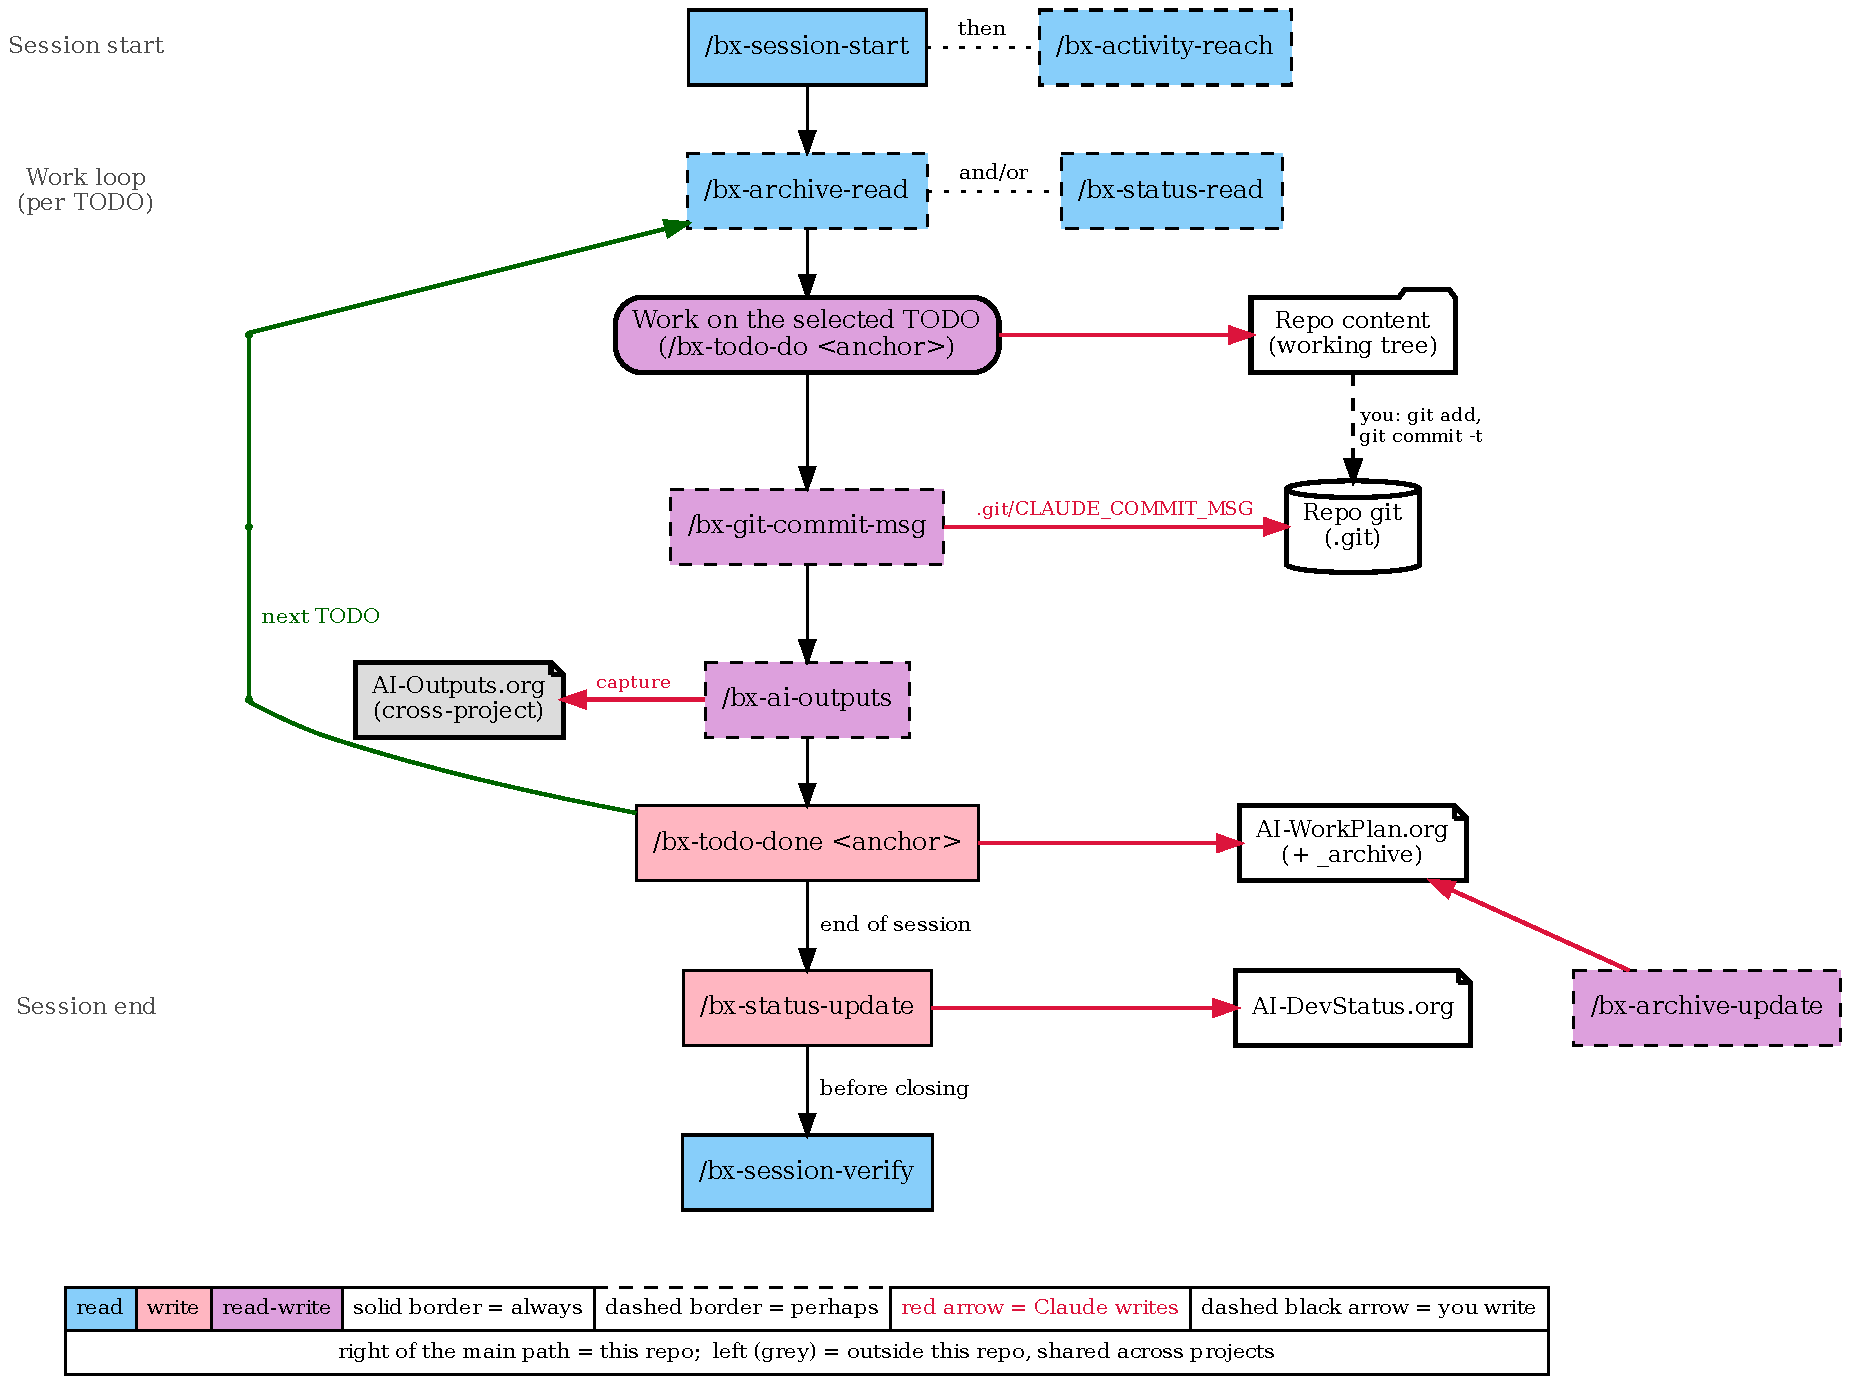
\includegraphics[width=\textwidth,height=0.95\textheight,keepaspectratio]{./figures/aiUsageWorkflow}
  \end{center}
\end{latexonly}
\begin{htmlonly}
  \begin{rawhtml}
<div class="center">
<img src="./figures/aiUsageWorkflow.png" height="450">
</div>
  \end{rawhtml}
\end{htmlonly}
\end{presentationMode}

\begin{articleMode}
  \begin{figure}[H]
    \begin{center}
      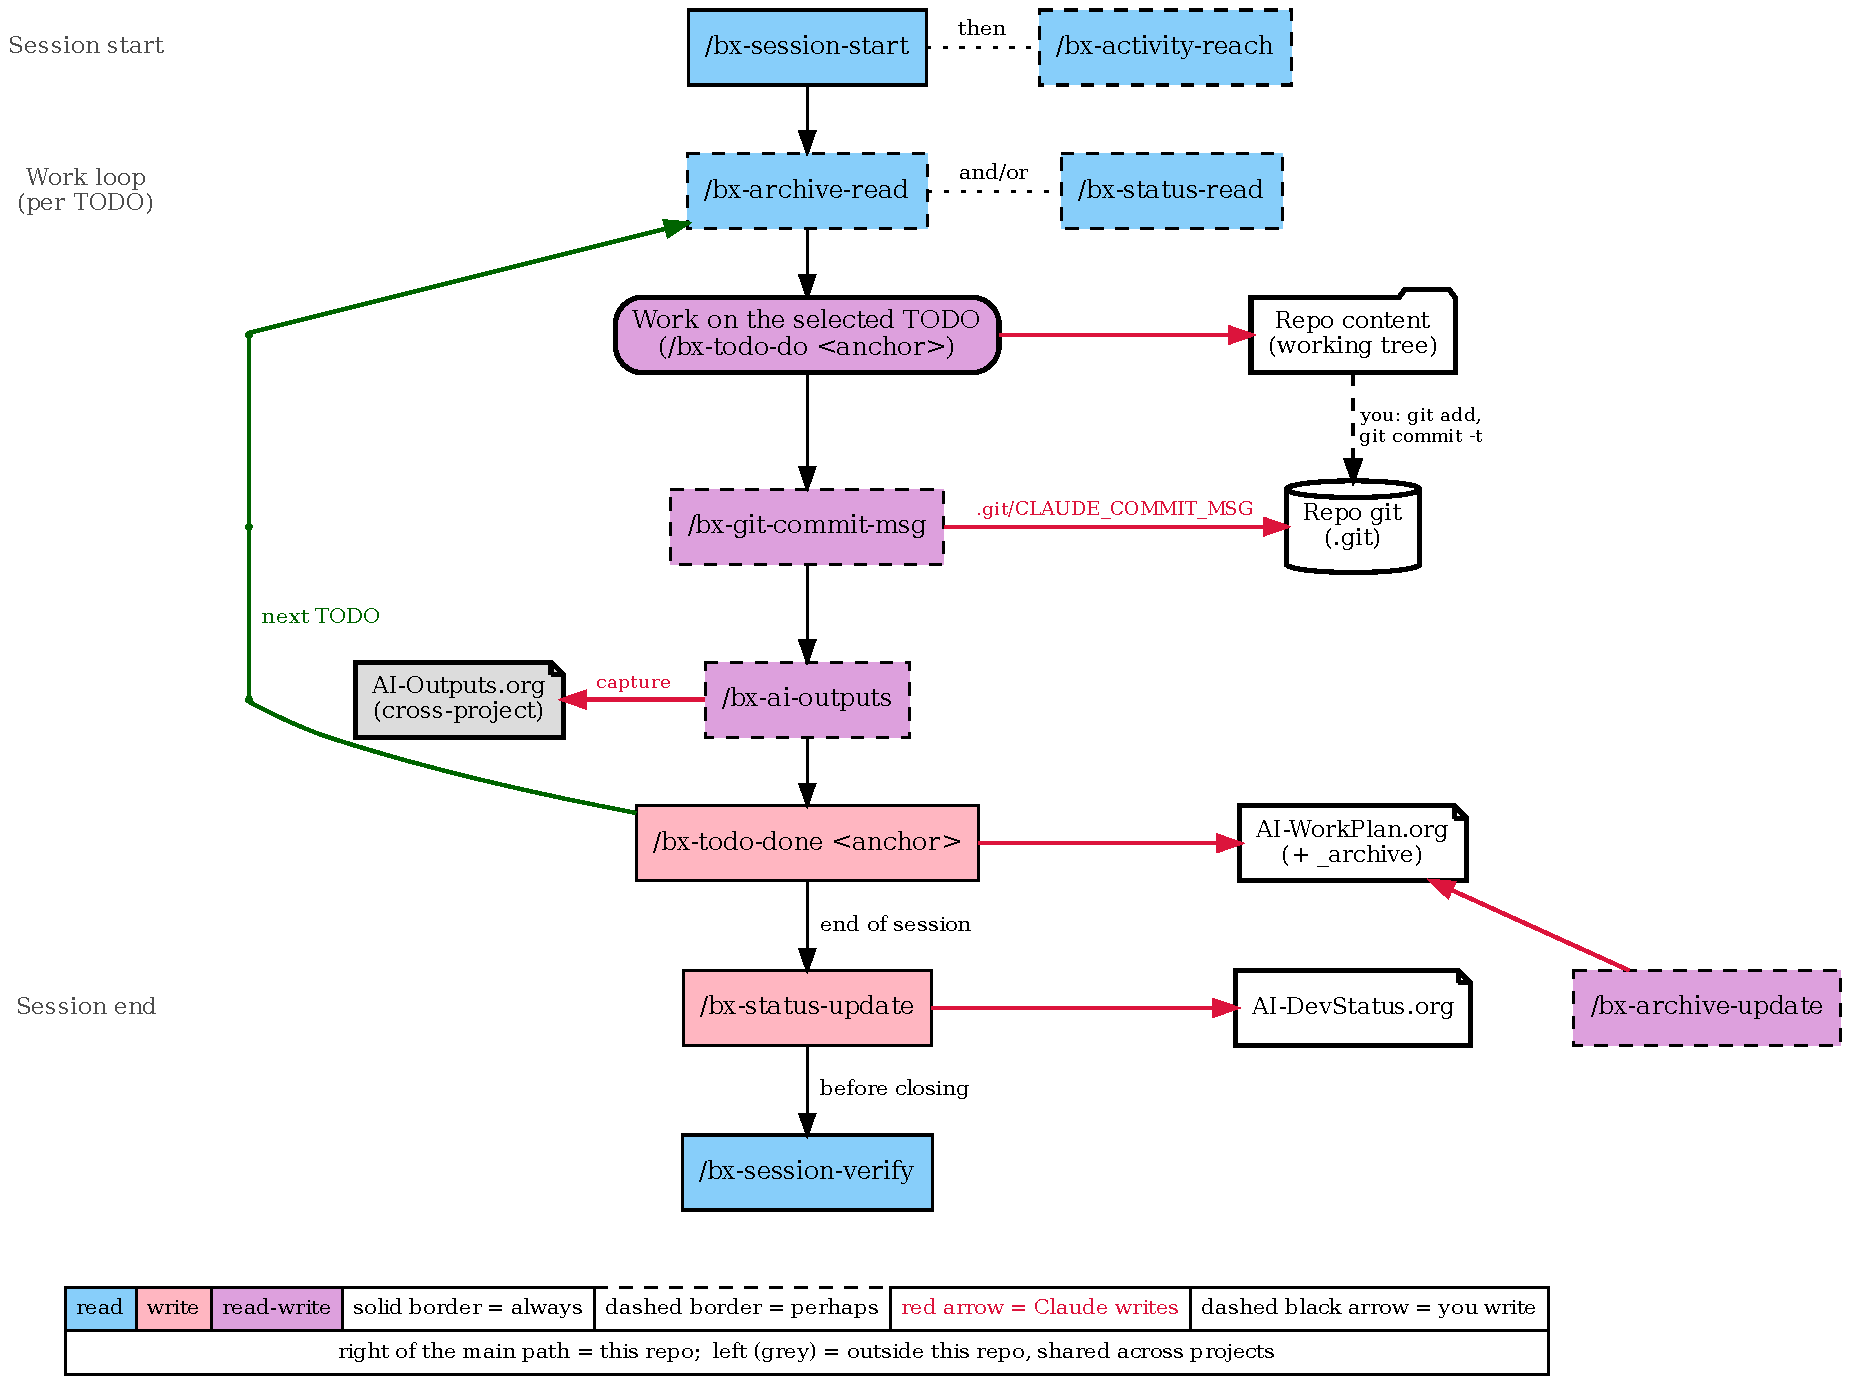
\includegraphics[width=\textwidth,height=0.8\textheight,keepaspectratio]{./figures/aiUsageWorkflow}
      \caption{AI-Activity Session Workflow}
      \label{fig:aiUsageWorkflow}
    \end{center}
  \end{figure}
\end{articleMode}

\pnote{

And this is a session: confirm the context at the start, a work loop per TODO,
and housekeeping at the end. The colors show what each command reads and writes.

}

\end{frame}
\end{verblatex}



%%%#+BEGIN: b:lcnt:pres:frame/derivedImage :title "The /bx- Commands Are the Workflow" :subtitle "" :label "bxCommands" :comment "body=itemize" :reveal "plain" :beamer "plain"
\begin{whenOrg}
*****  _[[elisp:(blee:menu-sel:outline:popupMenu)][±]]_ _[[elisp:(blee:menu-sel:navigation:popupMenu)][Ξ]]_ [[elisp:(outline-show-branches+toggle)][|=]] [[elisp:(bx:orgm:indirectBufOther)][|>]] *[[elisp:(blee:ppmm:org-mode-toggle)][|N]]*  derivedImage [[elisp:(outline-show-subtree+toggle)][||]] Label=bxCommands The /bx- Commands Are the Workflow body=itemize
\end{whenOrg}

\begin{htmlonly}

\begin{frame}[fragile,plain,label=bxCommands]
    \frameaudio{"audio/bxCommands.mp3"}
    \frametitle{}
    \framesubtitle{}
    \begin{rawhtml}
<div class="center">
<img src="./disposition.gened/bxCommands/slide-1.png" height="500">
</div>
    \end{rawhtml}
\end{frame}
\end{htmlonly}

\begin{verblatex}

\begin{frame}[fragile,plain,label=bxCommands]
    \frameaudio{"audio/bxCommands.mp3"}
    \frametitle{The /bx- Commands Are the Workflow}
    \framesubtitle{}
%%BxPy: impressiveFrameParSet('bxCommands', 'always', 'True')
%%BxPy: impressiveFrameParSet('bxCommands', 'transition', 'UnSpecified')
%%%#+END:

{\footnotesize \renewcommand{\arraystretch}{1.3}
  \begin{tabular}{|p{0.8in}|p{3.3in}|}
    \hline
    Session & session-start, session-report, session-verify \\
    \hline
    Activity & activity-reach, activity-report \\
    \hline
    Work & status-read, todo-do, todo-done \\
    \hline
    Record & status-update, archive-update, archive-read \\
    \hline
    Git & git-commit-msg, git-commit-walk, git-uncommitted-list \\
    \hline
    Findings & ai-outputs --- a cross-project ledger \\
    \hline
  \end{tabular}
  }

  \vspace{0.1in}
  One set for every activity. The human commits; the AI writes the commit message.

\pnote{

The slash commands are the workflow. One set, the same for every activity:
session, activity, work, record, git, and a cross-project ledger of findings.
The human does all commits; the AI writes the message.

}

\end{frame}
\end{verblatex}



%%%#+BEGIN: bx:dblock:lcnt:latex-section :mode "auto" :seg-title "Pairing Emacs and VS Code"
%%% Args: :class "book|pres+art" :langs "en+fa" :disabledP "false" :seg-title "str" :short-title "str" :label "auto"
\begin{whenOrg}
*  _[[elisp:(blee:menu-sel:outline:popupMenu)][±]]_ _[[elisp:(blee:menu-sel:navigation:popupMenu)][Ξ]]_ [[elisp:(outline-show-branches+toggle)][|=]] [[elisp:(bx:orgm:indirectBufOther)][|>]] *[[elisp:(blee:ppmm:org-mode-toggle)][|N]]*  Section    [[elisp:(outline-show-subtree+toggle)][||]]   /Pairing Emacs and VS Code/ ::  [[elisp:(org-cycle)][| ]]
\end{whenOrg}

\section{Pairing Emacs and VS Code}
%%%#+END:

%%%#+BEGIN: b:lcnt:pres:frame/derivedImage :title "Pairing Emacs and VS Code" :subtitle "" :label "emacsVscodePairing" :comment "body=figure" :reveal "plain" :beamer "plain"
\begin{whenOrg}
*****  _[[elisp:(blee:menu-sel:outline:popupMenu)][±]]_ _[[elisp:(blee:menu-sel:navigation:popupMenu)][Ξ]]_ [[elisp:(outline-show-branches+toggle)][|=]] [[elisp:(bx:orgm:indirectBufOther)][|>]] *[[elisp:(blee:ppmm:org-mode-toggle)][|N]]*  derivedImage [[elisp:(outline-show-subtree+toggle)][||]] Label=emacsVscodePairing Pairing Emacs and VS Code body=figure
\end{whenOrg}

\begin{htmlonly}

\begin{frame}[fragile,plain,label=emacsVscodePairing]
    \frameaudio{"audio/emacsVscodePairing.mp3"}
    \frametitle{}
    \framesubtitle{}
    \begin{rawhtml}
<div class="center">
<img src="./disposition.gened/emacsVscodePairing/slide-1.png" height="500">
</div>
    \end{rawhtml}
\end{frame}
\end{htmlonly}

\begin{verblatex}

\begin{frame}[fragile,plain,label=emacsVscodePairing]
    \frameaudio{"audio/emacsVscodePairing.mp3"}
    \frametitle{Pairing Emacs and VS Code}
    \framesubtitle{}
%%BxPy: impressiveFrameParSet('emacsVscodePairing', 'always', 'True')
%%BxPy: impressiveFrameParSet('emacsVscodePairing', 'transition', 'UnSpecified')
%%%#+END:

\begin{presentationMode}
\begin{latexonly}
  \vspace*{-0.25in}
  \begin{center}
    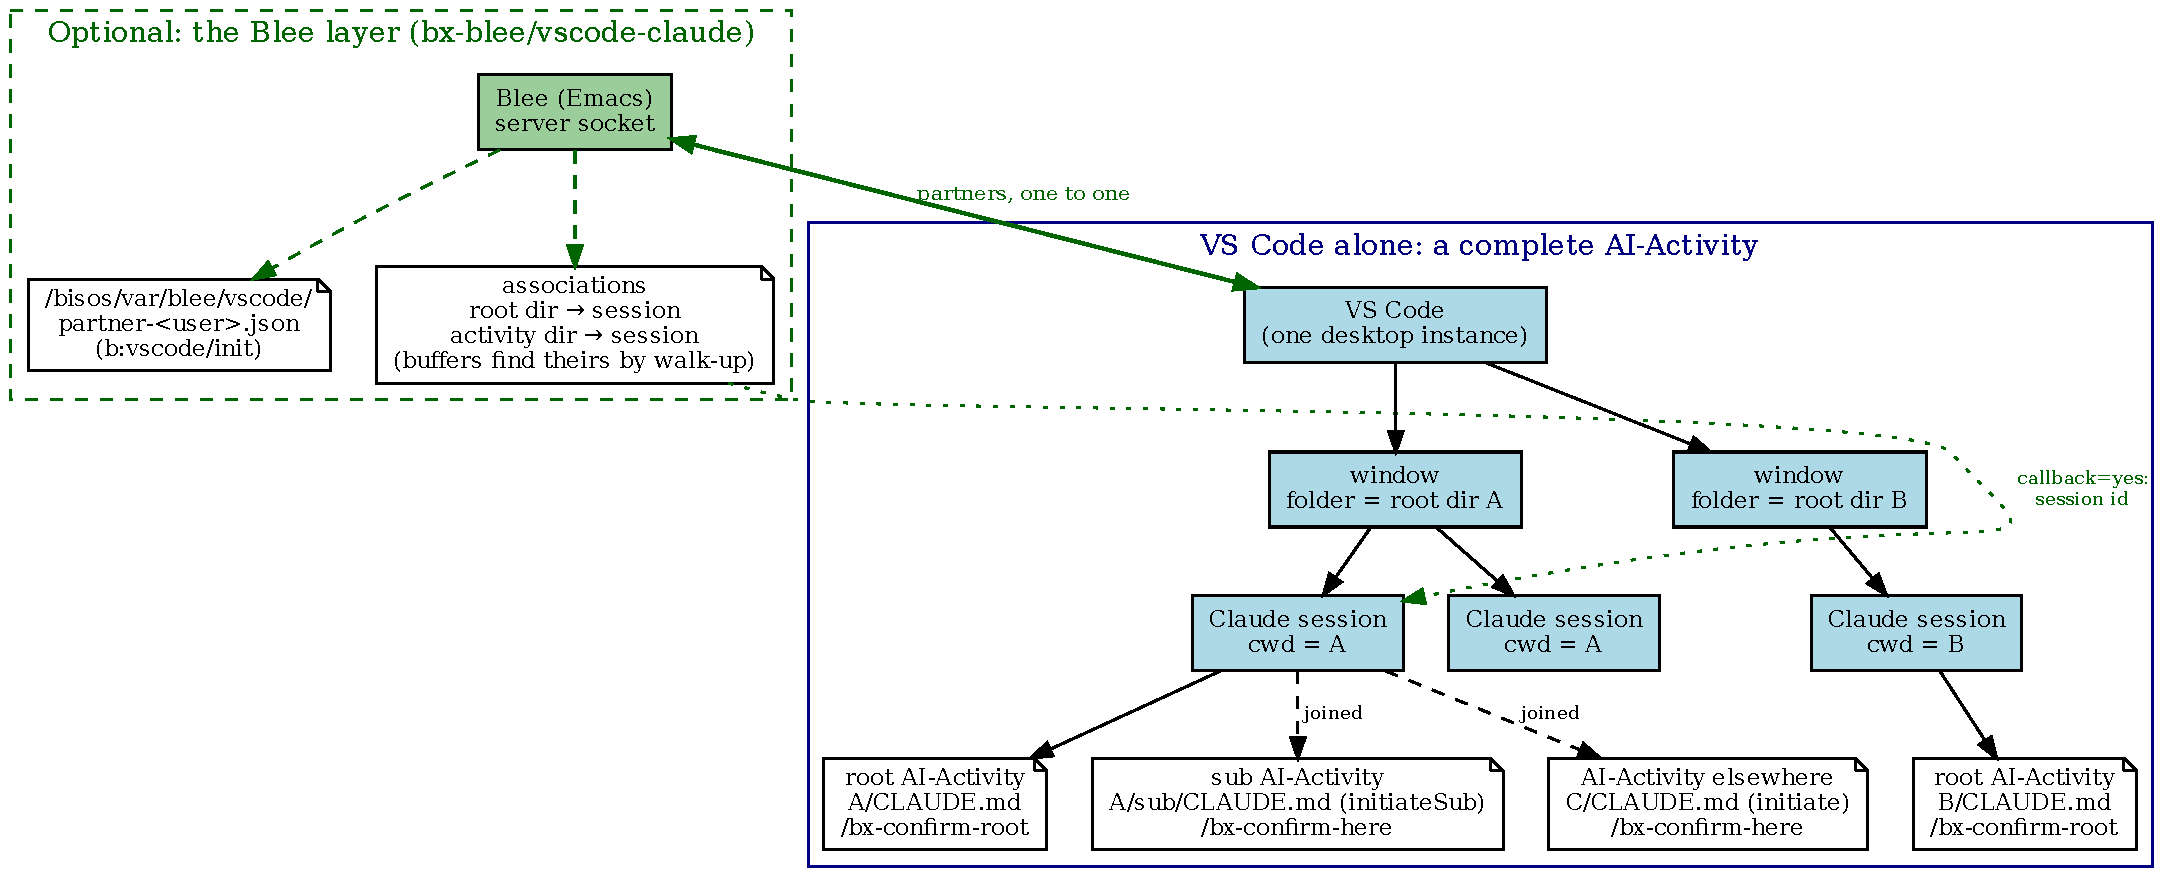
\includegraphics[width=\textwidth,height=0.95\textheight,keepaspectratio]{./figures/vscodeClaudeHierarchy}
  \end{center}
\end{latexonly}
\begin{htmlonly}
  \begin{rawhtml}
<div class="center">
<img src="./figures/vscodeClaudeHierarchy.png" height="450">
</div>
  \end{rawhtml}
\end{htmlonly}
\end{presentationMode}

\begin{articleMode}
  \begin{figure}[H]
    \begin{center}
      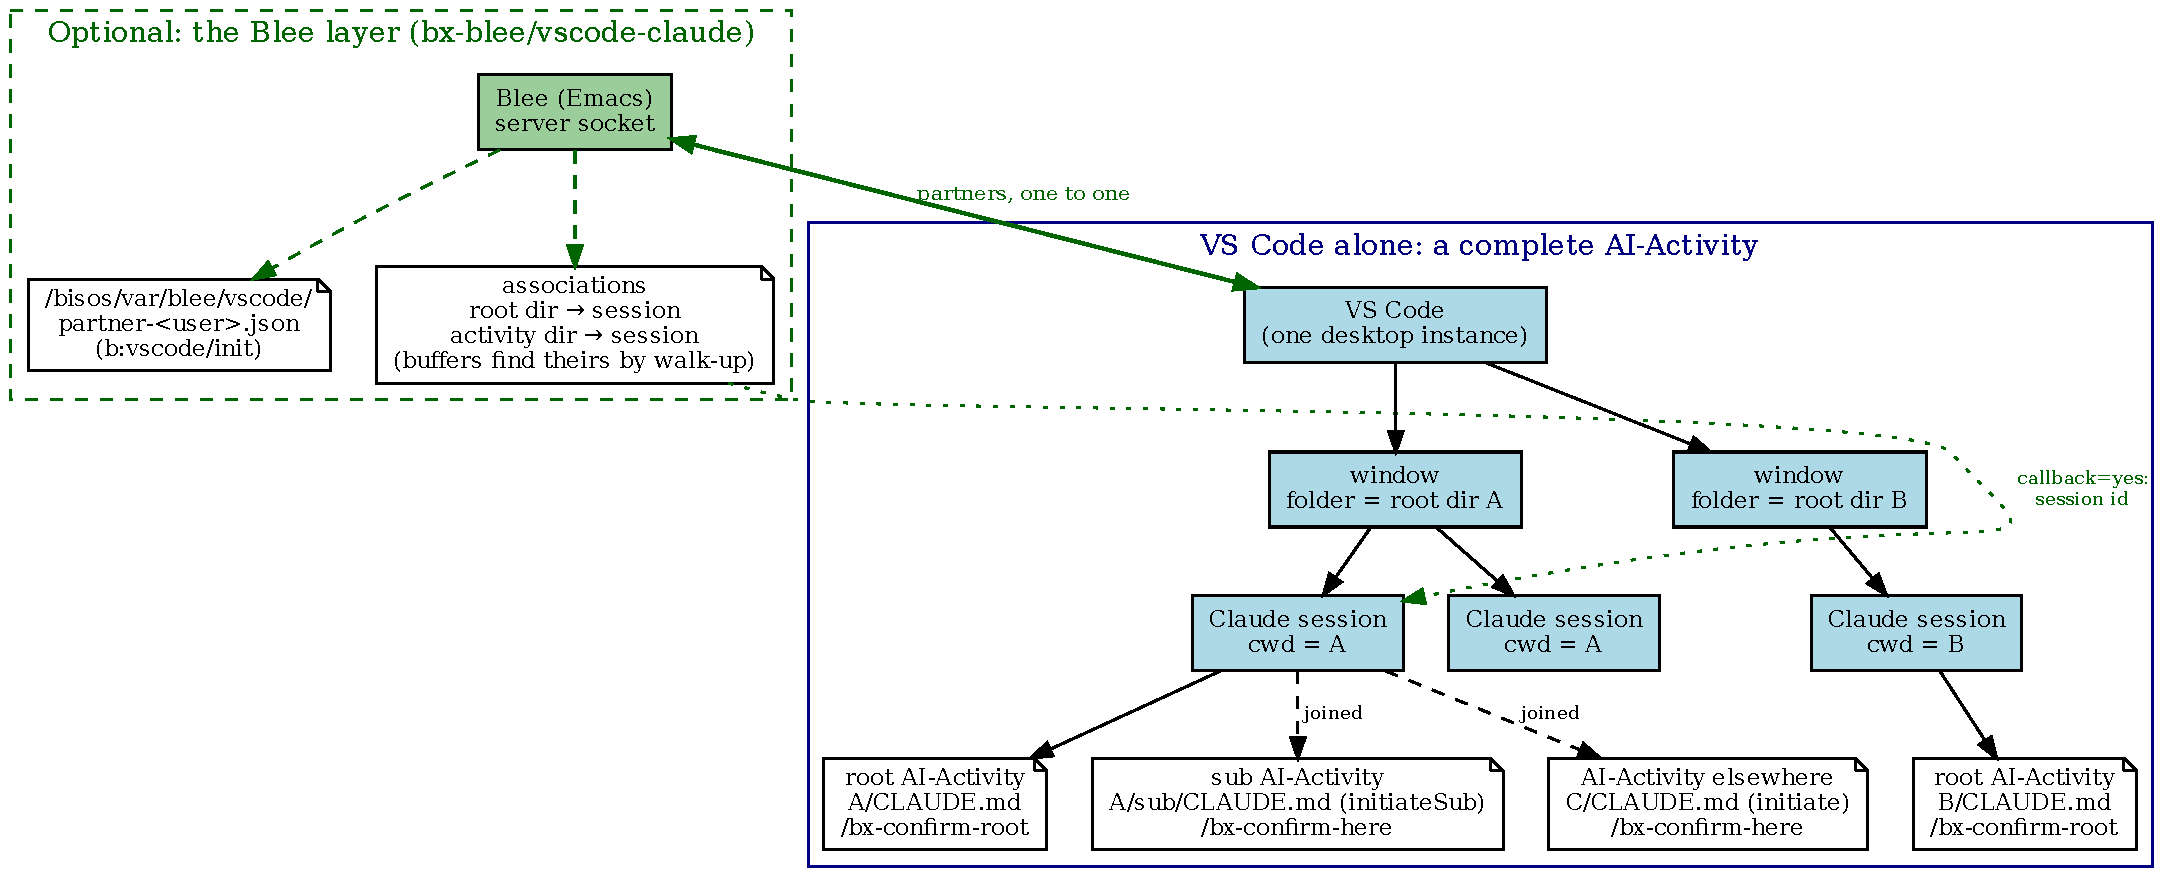
\includegraphics[width=\textwidth,height=0.8\textheight,keepaspectratio]{./figures/vscodeClaudeHierarchy}
      \caption{Emacs, VS Code, Claude Sessions and AI-Activities}
      \label{fig:vscodeClaudeHierarchy}
    \end{center}
  \end{figure}
\end{articleMode}

\pnote{

In my own use, one Emacs partners with one VS Code instance.
A VS Code window's folder is the root of its Claude sessions, and each session
holds a hierarchy of AI-Activities. The Emacs side is optional.

}

\end{frame}
\end{verblatex}



%%%#+BEGIN: b:lcnt:pres:frame/derivedImage :title "The Channels Between Blee and VS Code Claude" :subtitle "" :label "emacsVscodeChannels" :comment "body=figure" :reveal "plain" :beamer "plain"
\begin{whenOrg}
*****  _[[elisp:(blee:menu-sel:outline:popupMenu)][±]]_ _[[elisp:(blee:menu-sel:navigation:popupMenu)][Ξ]]_ [[elisp:(outline-show-branches+toggle)][|=]] [[elisp:(bx:orgm:indirectBufOther)][|>]] *[[elisp:(blee:ppmm:org-mode-toggle)][|N]]*  derivedImage [[elisp:(outline-show-subtree+toggle)][||]] Label=emacsVscodeChannels The Channels Between Blee and VS Code Claude body=figure
\end{whenOrg}

\begin{htmlonly}

\begin{frame}[fragile,plain,label=emacsVscodeChannels]
    \frameaudio{"audio/emacsVscodeChannels.mp3"}
    \frametitle{}
    \framesubtitle{}
    \begin{rawhtml}
<div class="center">
<img src="./disposition.gened/emacsVscodeChannels/slide-1.png" height="500">
</div>
    \end{rawhtml}
\end{frame}
\end{htmlonly}

\begin{verblatex}

\begin{frame}[fragile,plain,label=emacsVscodeChannels]
    \frameaudio{"audio/emacsVscodeChannels.mp3"}
    \frametitle{The Channels Between Blee and VS Code Claude}
    \framesubtitle{}
%%BxPy: impressiveFrameParSet('emacsVscodeChannels', 'always', 'True')
%%BxPy: impressiveFrameParSet('emacsVscodeChannels', 'transition', 'UnSpecified')
%%%#+END:

\begin{presentationMode}
\begin{latexonly}
  \vspace*{-0.25in}
  \begin{center}
    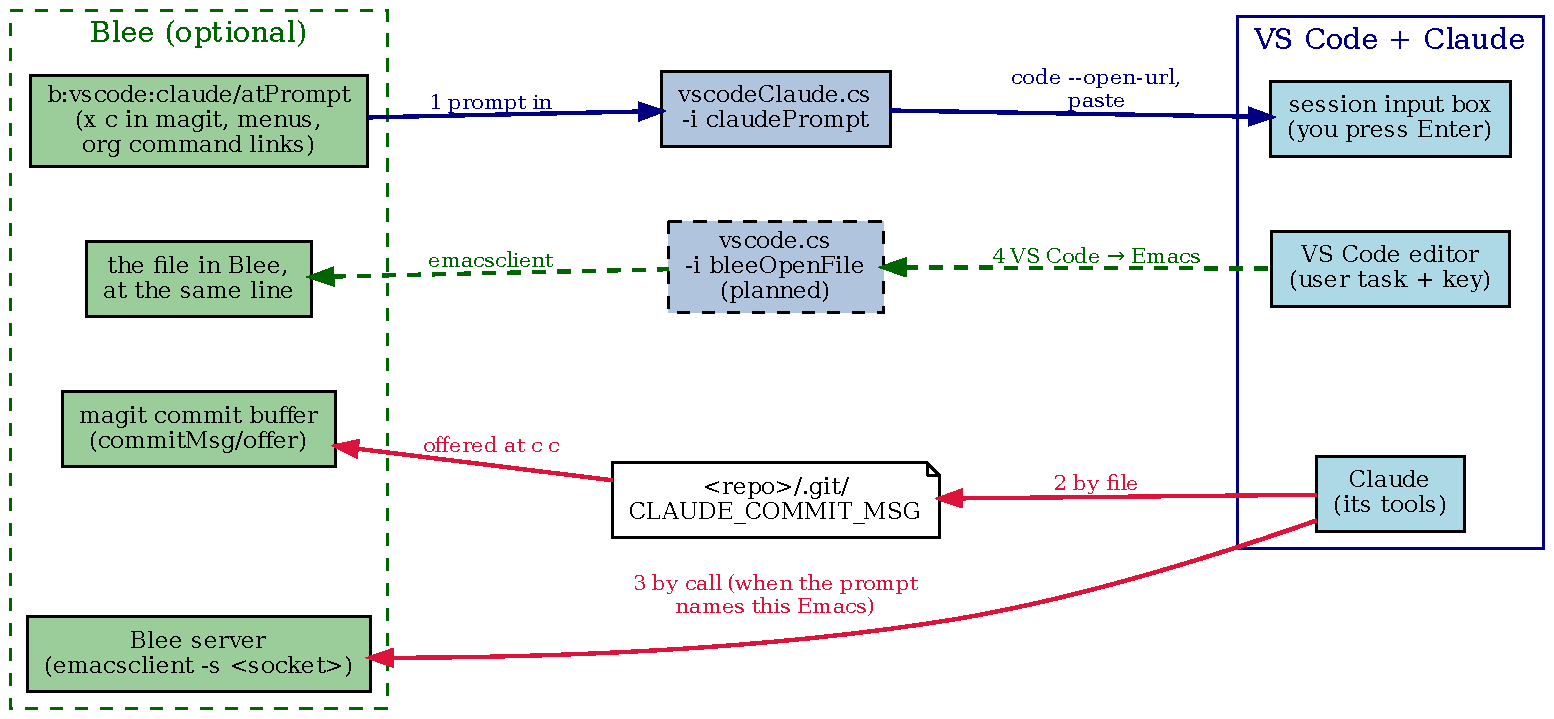
\includegraphics[width=\textwidth,height=0.95\textheight,keepaspectratio]{./figures/vscodeClaudeChannels}
  \end{center}
\end{latexonly}
\begin{htmlonly}
  \begin{rawhtml}
<div class="center">
<img src="./figures/vscodeClaudeChannels.png" height="450">
</div>
  \end{rawhtml}
\end{htmlonly}
\end{presentationMode}

\begin{articleMode}
  \begin{figure}[H]
    \begin{center}
      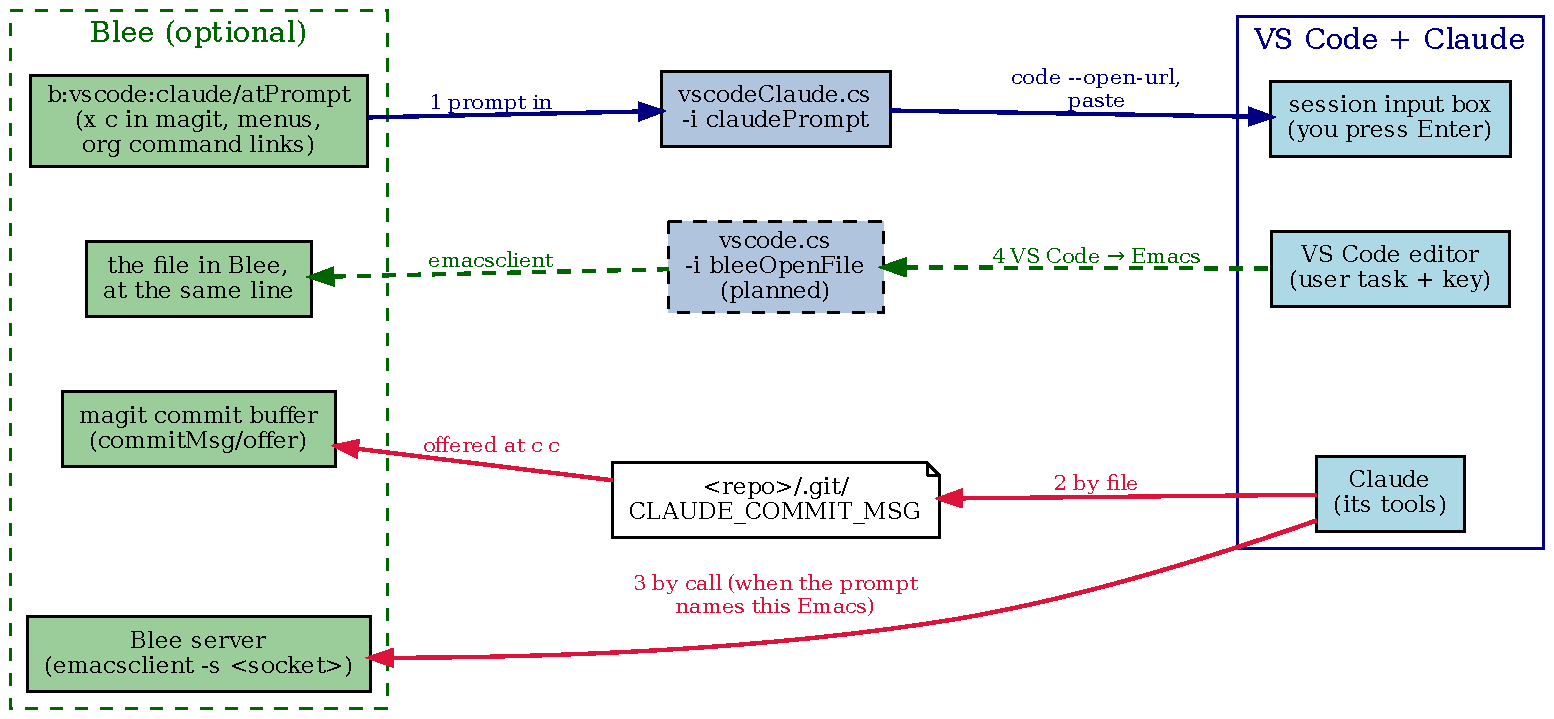
\includegraphics[width=\textwidth,height=0.8\textheight,keepaspectratio]{./figures/vscodeClaudeChannels}
      \caption{The Channels Between Blee and VS Code Claude}
      \label{fig:vscodeClaudeChannels}
    \end{center}
  \end{figure}
\end{articleMode}

\pnote{

Emacs sends prompts into a session; results come back by file,
or by a call into that Emacs when the prompt names it.

}

\end{frame}
\end{verblatex}



%%%#+BEGIN: b:lcnt:pres:frame/derivedImage :title "Layers: Emacs Is Optional" :subtitle "" :label "vscodeClaudeLayers" :comment "body=figure" :reveal "plain" :beamer "plain"
\begin{whenOrg}
*****  _[[elisp:(blee:menu-sel:outline:popupMenu)][±]]_ _[[elisp:(blee:menu-sel:navigation:popupMenu)][Ξ]]_ [[elisp:(outline-show-branches+toggle)][|=]] [[elisp:(bx:orgm:indirectBufOther)][|>]] *[[elisp:(blee:ppmm:org-mode-toggle)][|N]]*  derivedImage [[elisp:(outline-show-subtree+toggle)][||]] Label=vscodeClaudeLayers Layers: Emacs Is Optional body=figure
\end{whenOrg}

\begin{htmlonly}

\begin{frame}[fragile,plain,label=vscodeClaudeLayers]
    \frameaudio{"audio/vscodeClaudeLayers.mp3"}
    \frametitle{}
    \framesubtitle{}
    \begin{rawhtml}
<div class="center">
<img src="./disposition.gened/vscodeClaudeLayers/slide-1.png" height="500">
</div>
    \end{rawhtml}
\end{frame}
\end{htmlonly}

\begin{verblatex}

\begin{frame}[fragile,plain,label=vscodeClaudeLayers]
    \frameaudio{"audio/vscodeClaudeLayers.mp3"}
    \frametitle{Layers: Emacs Is Optional}
    \framesubtitle{}
%%BxPy: impressiveFrameParSet('vscodeClaudeLayers', 'always', 'True')
%%BxPy: impressiveFrameParSet('vscodeClaudeLayers', 'transition', 'UnSpecified')
%%%#+END:

\begin{presentationMode}
\begin{latexonly}
  \vspace*{-0.25in}
  \begin{center}
    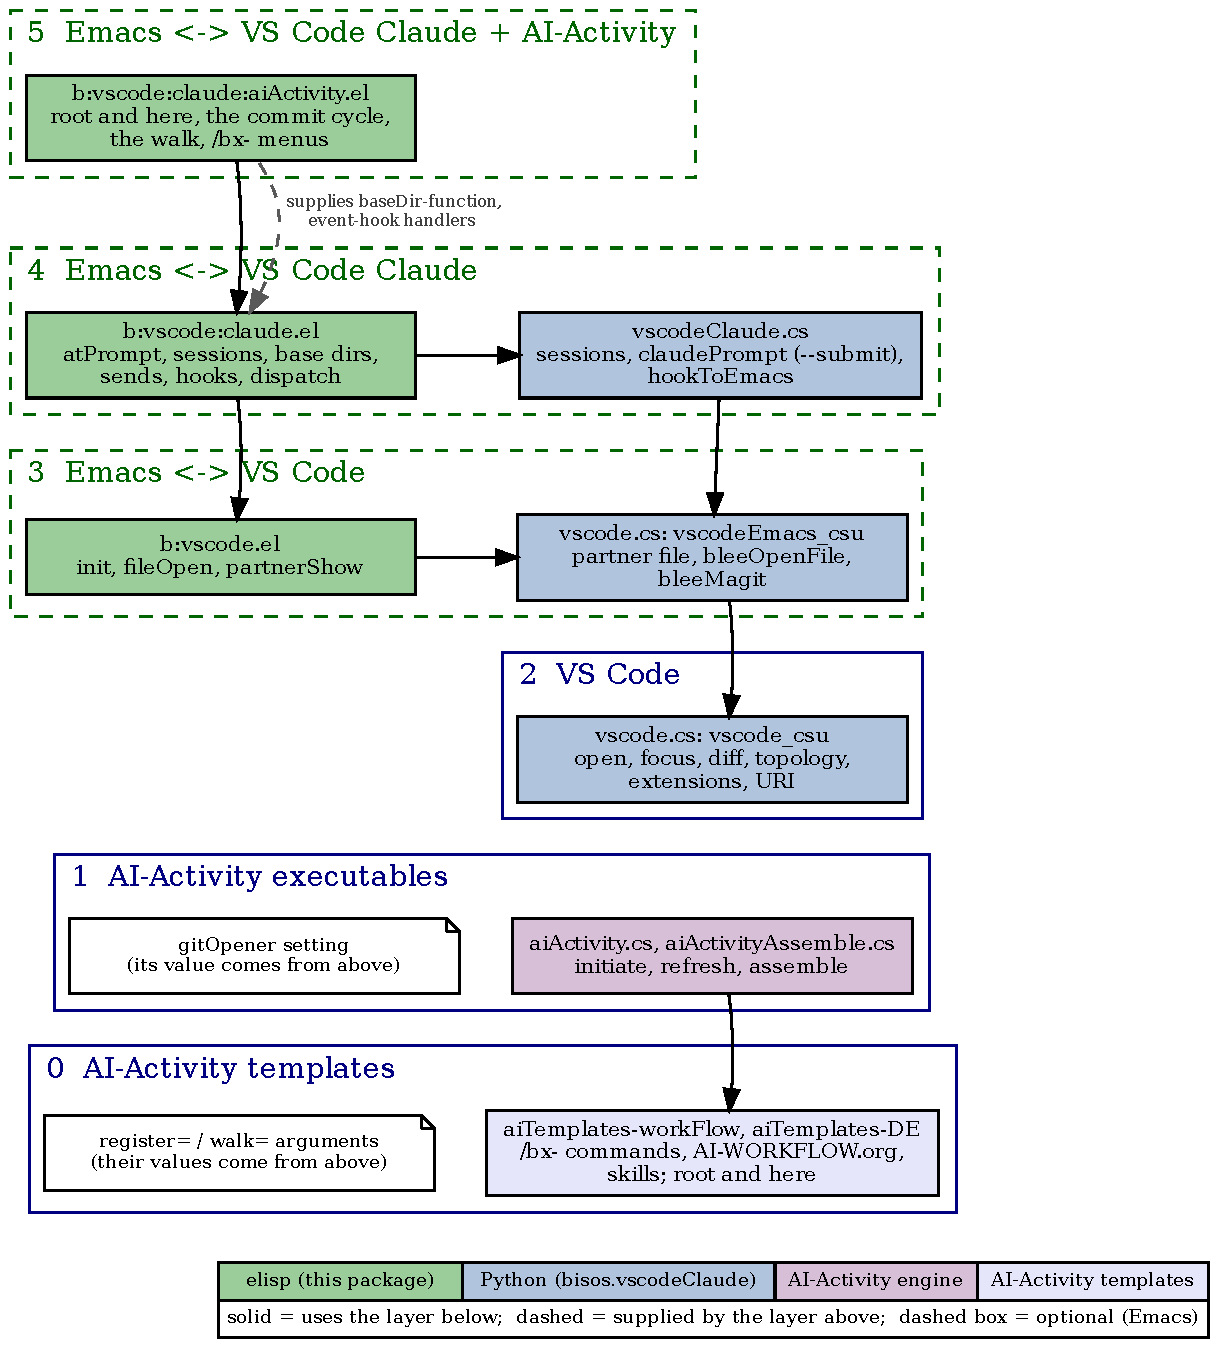
\includegraphics[width=\textwidth,height=0.95\textheight,keepaspectratio]{./figures/vscodeClaudeLayers}
  \end{center}
\end{latexonly}
\begin{htmlonly}
  \begin{rawhtml}
<div class="center">
<img src="./figures/vscodeClaudeLayers.png" height="450">
</div>
  \end{rawhtml}
\end{htmlonly}
\end{presentationMode}

\begin{articleMode}
  \begin{figure}[H]
    \begin{center}
      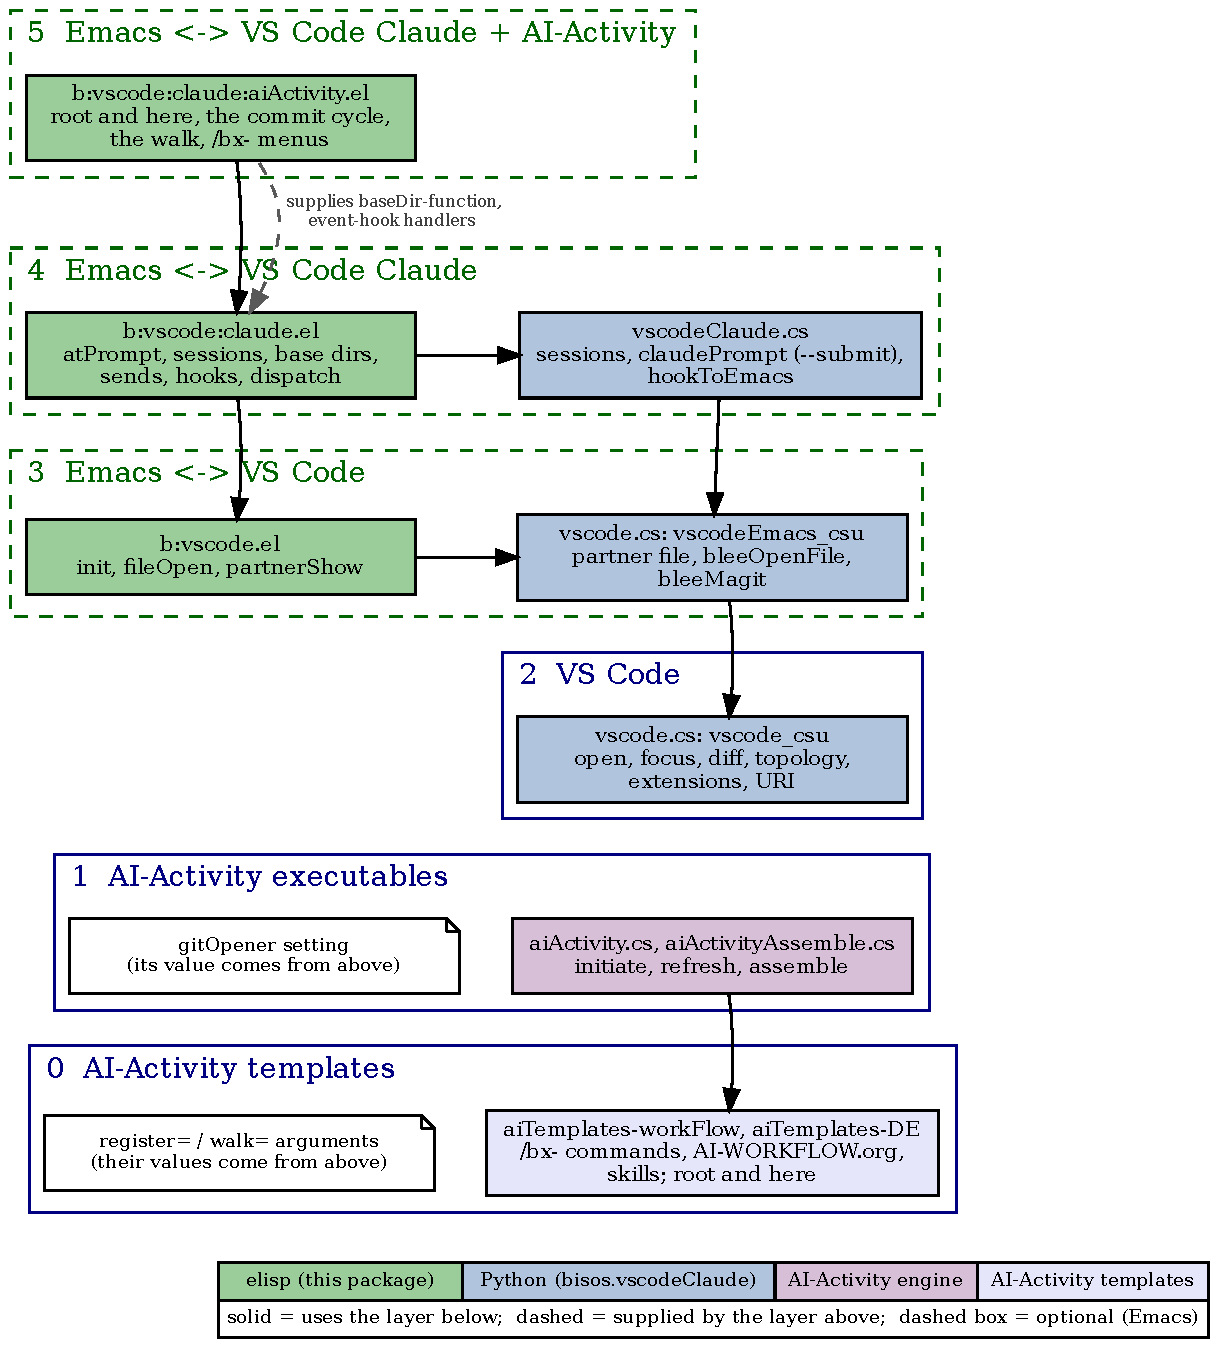
\includegraphics[width=\textwidth,height=0.8\textheight,keepaspectratio]{./figures/vscodeClaudeLayers}
      \caption{The Six Layers of vscode-claude}
      \label{fig:vscodeClaudeLayers}
    \end{center}
  \end{figure}
\end{articleMode}

\pnote{

These are layered so that each layer is usable with only the layers below it:
the templates, their executables, VS Code, and then Emacs. A pure VS Code user loses nothing.

}

\end{frame}
\end{verblatex}



%%%#+BEGIN: bx:dblock:lcnt:latex-section :mode "auto" :seg-title "Agent-Neutral Content"
%%% Args: :class "book|pres+art" :langs "en+fa" :disabledP "false" :seg-title "str" :short-title "str" :label "auto"
\begin{whenOrg}
*  _[[elisp:(blee:menu-sel:outline:popupMenu)][±]]_ _[[elisp:(blee:menu-sel:navigation:popupMenu)][Ξ]]_ [[elisp:(outline-show-branches+toggle)][|=]] [[elisp:(bx:orgm:indirectBufOther)][|>]] *[[elisp:(blee:ppmm:org-mode-toggle)][|N]]*  Section    [[elisp:(outline-show-subtree+toggle)][||]]   /Agent-Neutral Content/ ::  [[elisp:(org-cycle)][| ]]
\end{whenOrg}

\section{Agent-Neutral Content}
%%%#+END:

%%%#+BEGIN: b:lcnt:pres:frame/derivedImage :title "Agent-Neutral Content, a Thin Claude Binding" :subtitle "" :label "agentNeutral" :comment "body=itemize" :reveal "plain" :beamer "plain"
\begin{whenOrg}
*****  _[[elisp:(blee:menu-sel:outline:popupMenu)][±]]_ _[[elisp:(blee:menu-sel:navigation:popupMenu)][Ξ]]_ [[elisp:(outline-show-branches+toggle)][|=]] [[elisp:(bx:orgm:indirectBufOther)][|>]] *[[elisp:(blee:ppmm:org-mode-toggle)][|N]]*  derivedImage [[elisp:(outline-show-subtree+toggle)][||]] Label=agentNeutral Agent-Neutral Content, a Thin Claude Binding body=itemize
\end{whenOrg}

\begin{htmlonly}

\begin{frame}[fragile,plain,label=agentNeutral]
    \frameaudio{"audio/agentNeutral.mp3"}
    \frametitle{}
    \framesubtitle{}
    \begin{rawhtml}
<div class="center">
<img src="./disposition.gened/agentNeutral/slide-1.png" height="500">
</div>
    \end{rawhtml}
\end{frame}
\end{htmlonly}

\begin{verblatex}

\begin{frame}[fragile,plain,label=agentNeutral]
    \frameaudio{"audio/agentNeutral.mp3"}
    \frametitle{Agent-Neutral Content, a Thin Claude Binding}
    \framesubtitle{}
%%BxPy: impressiveFrameParSet('agentNeutral', 'always', 'True')
%%BxPy: impressiveFrameParSet('agentNeutral', 'transition', 'UnSpecified')
%%%#+END:

\begin{itemize}
  \item Only the file names Claude Code looks for are Claude's:
    \begin{itemize}
    \item \texttt{CLAUDE.md} and \texttt{.claude/}
    \end{itemize}
  \item Everything else is plain org-mode, owned by you
    \begin{itemize}
    \item Activities, plans, status, skills
    \end{itemize}
  \item The context survives a change of AI-Assistant
  \end{itemize}

\pnote{

Only the file names that Claude Code looks for are specific to Claude.
Everything else is plain org-mode that you own, so the context survives
a change of AI assistant.

}

\end{frame}
\end{verblatex}



%%%#+BEGIN: bx:dblock:lcnt:latex-part :disabledP "false" :seg-title "ByStar, BISOS and Blee as Digital Ecosystem Skills"
%%% Args: :toc "NU" :tocDepth 3 :part "NU" :label "auto|spec" :partpage t
\begin{whenOrg}
*      ================
*  [[elisp:(blee:ppmm:org-mode-toggle)][|n]] [[elisp:(blee:menu-sel:outline:popupMenu)][+-]] [[elisp:(blee:menu-sel:navigation:popupMenu)][==]]  *Part*   _ByStar, BISOS and Blee as Digital Ecosystem Skills_ ::  [[elisp:(org-cycle)][| ]]
\end{whenOrg}

\newpage
\part{ByStar, BISOS and Blee as Digital Ecosystem Skills}
%%%#+END:

%%%#+BEGIN: bx:dblock:lcnt:latex-section :mode "auto" :seg-title "Workflow Plus Ecosystem"
%%% Args: :class "book|pres+art" :langs "en+fa" :disabledP "false" :seg-title "str" :short-title "str" :label "auto"
\begin{whenOrg}
*  _[[elisp:(blee:menu-sel:outline:popupMenu)][±]]_ _[[elisp:(blee:menu-sel:navigation:popupMenu)][Ξ]]_ [[elisp:(outline-show-branches+toggle)][|=]] [[elisp:(bx:orgm:indirectBufOther)][|>]] *[[elisp:(blee:ppmm:org-mode-toggle)][|N]]*  Section    [[elisp:(outline-show-subtree+toggle)][||]]   /Workflow Plus Ecosystem/ ::  [[elisp:(org-cycle)][| ]]
\end{whenOrg}

\section{Workflow Plus Ecosystem}
%%%#+END:

%%%#+BEGIN: b:lcnt:pres:frame/derivedImage :title "Templates: The Workflow Plus an Ecosystem" :subtitle "" :label "assembleTemplates" :comment "body=figure" :reveal "plain" :beamer "plain"
\begin{whenOrg}
*****  _[[elisp:(blee:menu-sel:outline:popupMenu)][±]]_ _[[elisp:(blee:menu-sel:navigation:popupMenu)][Ξ]]_ [[elisp:(outline-show-branches+toggle)][|=]] [[elisp:(bx:orgm:indirectBufOther)][|>]] *[[elisp:(blee:ppmm:org-mode-toggle)][|N]]*  derivedImage [[elisp:(outline-show-subtree+toggle)][||]] Label=assembleTemplates Templates: The Workflow Plus an Ecosystem body=figure
\end{whenOrg}

\begin{htmlonly}

\begin{frame}[fragile,plain,label=assembleTemplates]
    \frameaudio{"audio/assembleTemplates.mp3"}
    \frametitle{}
    \framesubtitle{}
    \begin{rawhtml}
<div class="center">
<img src="./disposition.gened/assembleTemplates/slide-1.png" height="500">
</div>
    \end{rawhtml}
\end{frame}
\end{htmlonly}

\begin{verblatex}

\begin{frame}[fragile,plain,label=assembleTemplates]
    \frameaudio{"audio/assembleTemplates.mp3"}
    \frametitle{Templates: The Workflow Plus an Ecosystem}
    \framesubtitle{}
%%BxPy: impressiveFrameParSet('assembleTemplates', 'always', 'True')
%%BxPy: impressiveFrameParSet('assembleTemplates', 'transition', 'UnSpecified')
%%%#+END:

\begin{presentationMode}
\begin{latexonly}
  \vspace*{-0.25in}
  \begin{center}
    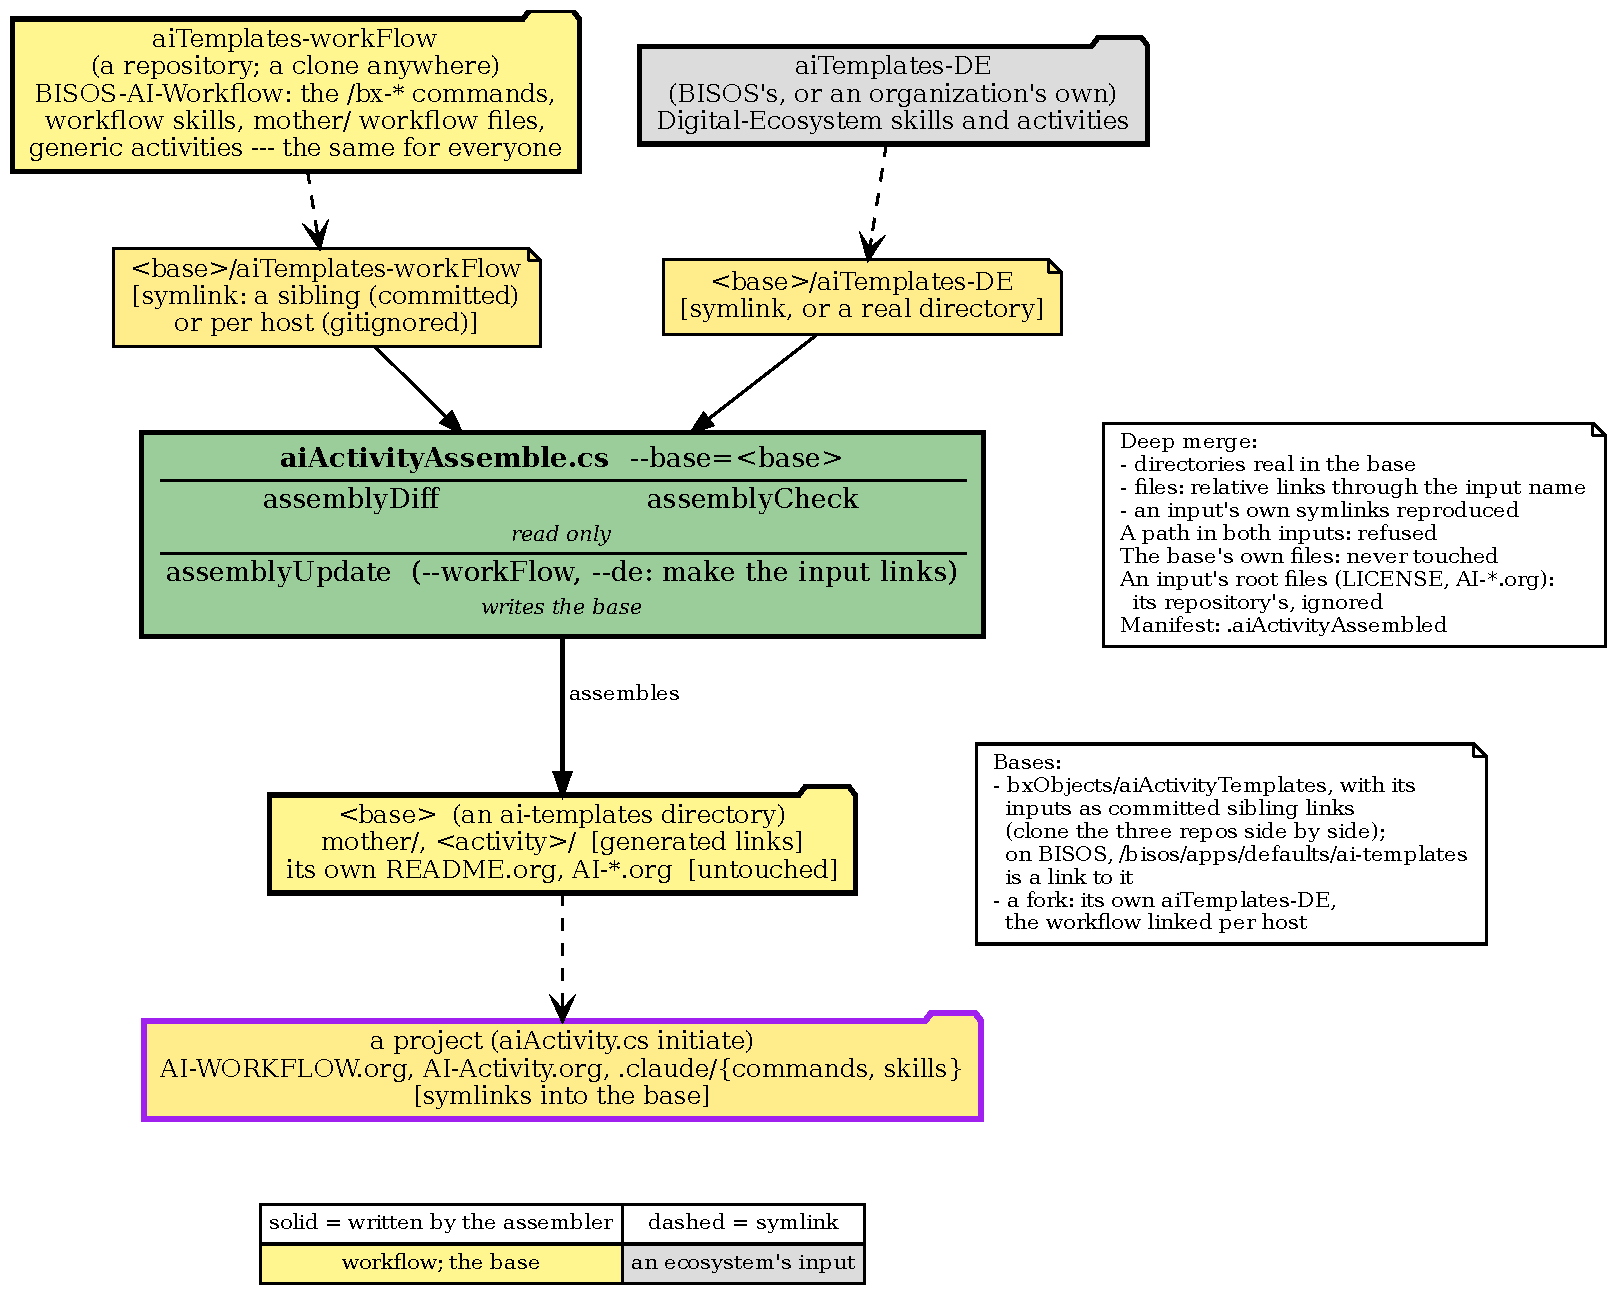
\includegraphics[width=\textwidth,height=0.95\textheight,keepaspectratio]{./figures/aiActivityAssembleFlow}
  \end{center}
\end{latexonly}
\begin{htmlonly}
  \begin{rawhtml}
<div class="center">
<img src="./figures/aiActivityAssembleFlow.png" height="450">
</div>
  \end{rawhtml}
\end{htmlonly}
\end{presentationMode}

\begin{articleMode}
  \begin{figure}[H]
    \begin{center}
      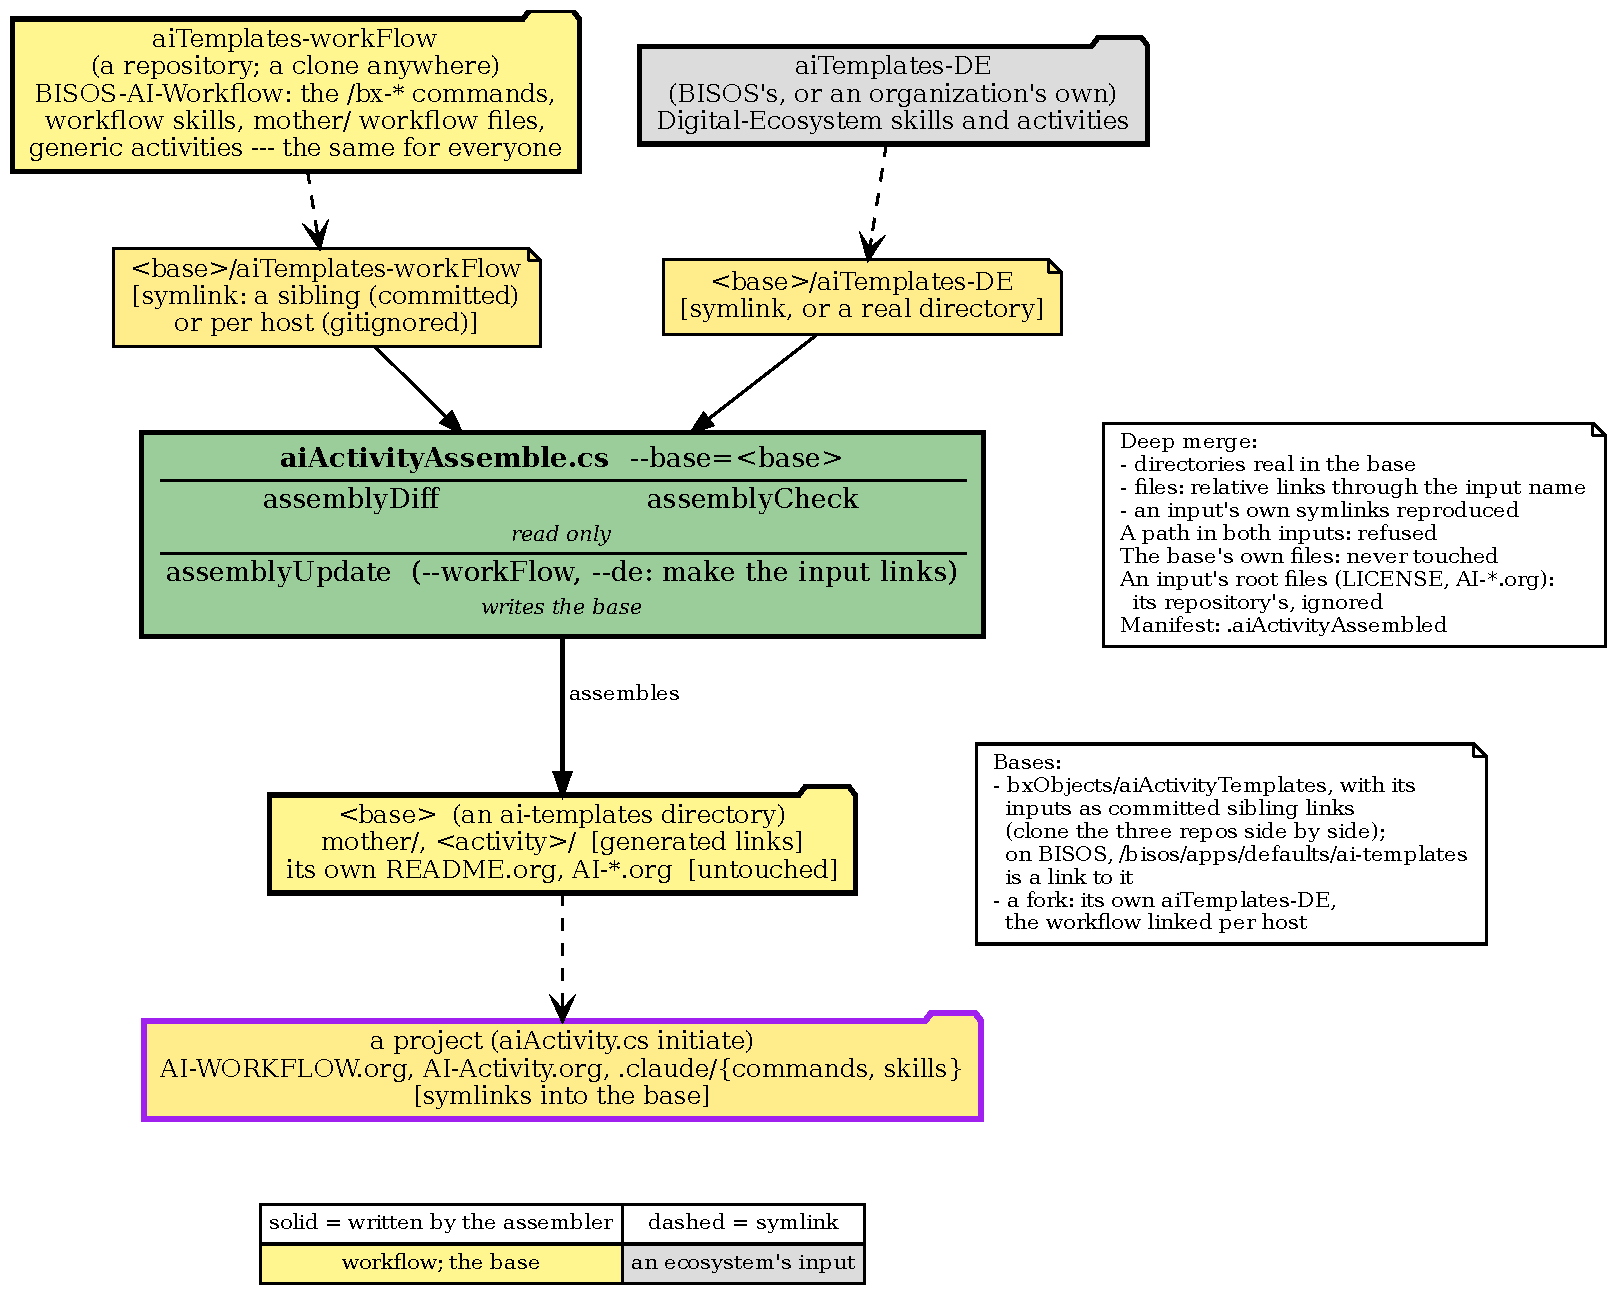
\includegraphics[width=\textwidth,height=0.8\textheight,keepaspectratio]{./figures/aiActivityAssembleFlow}
      \caption{Assembling a Templates Base}
      \label{fig:aiActivityAssembleFlow}
    \end{center}
  \end{figure}
\end{articleMode}

\pnote{

A templates base is assembled from two inputs. The workflow, the same for everyone.
And an ecosystem's own skills and activities. Ours are those of ByStar, BISOS and Blee.

}

\end{frame}
\end{verblatex}



%%%#+BEGIN: bx:dblock:lcnt:latex-section :mode "auto" :seg-title "BISOS Digital Ecosystem Skills"
%%% Args: :class "book|pres+art" :langs "en+fa" :disabledP "false" :seg-title "str" :short-title "str" :label "auto"
\begin{whenOrg}
*  _[[elisp:(blee:menu-sel:outline:popupMenu)][±]]_ _[[elisp:(blee:menu-sel:navigation:popupMenu)][Ξ]]_ [[elisp:(outline-show-branches+toggle)][|=]] [[elisp:(bx:orgm:indirectBufOther)][|>]] *[[elisp:(blee:ppmm:org-mode-toggle)][|N]]*  Section    [[elisp:(outline-show-subtree+toggle)][||]]   /BISOS Digital Ecosystem Skills/ ::  [[elisp:(org-cycle)][| ]]
\end{whenOrg}

\section{BISOS Digital Ecosystem Skills}
%%%#+END:

%%%#+BEGIN: b:lcnt:pres:frame/derivedImage :title "BISOS Digital Ecosystem Skills" :subtitle "" :label "ecosystemSkills" :comment "body=figure" :reveal "plain" :beamer "plain"
\begin{whenOrg}
*****  _[[elisp:(blee:menu-sel:outline:popupMenu)][±]]_ _[[elisp:(blee:menu-sel:navigation:popupMenu)][Ξ]]_ [[elisp:(outline-show-branches+toggle)][|=]] [[elisp:(bx:orgm:indirectBufOther)][|>]] *[[elisp:(blee:ppmm:org-mode-toggle)][|N]]*  derivedImage [[elisp:(outline-show-subtree+toggle)][||]] Label=ecosystemSkills BISOS Digital Ecosystem Skills body=figure
\end{whenOrg}

\begin{htmlonly}

\begin{frame}[fragile,plain,label=ecosystemSkills]
    \frameaudio{"audio/ecosystemSkills.mp3"}
    \frametitle{}
    \framesubtitle{}
    \begin{rawhtml}
<div class="center">
<img src="./disposition.gened/ecosystemSkills/slide-1.png" height="500">
</div>
    \end{rawhtml}
\end{frame}
\end{htmlonly}

\begin{verblatex}

\begin{frame}[fragile,plain,label=ecosystemSkills]
    \frameaudio{"audio/ecosystemSkills.mp3"}
    \frametitle{BISOS Digital Ecosystem Skills}
    \framesubtitle{}
%%BxPy: impressiveFrameParSet('ecosystemSkills', 'always', 'True')
%%BxPy: impressiveFrameParSet('ecosystemSkills', 'transition', 'UnSpecified')
%%%#+END:

\begin{presentationMode}
\begin{latexonly}
  \vspace*{-0.25in}
  \begin{center}
    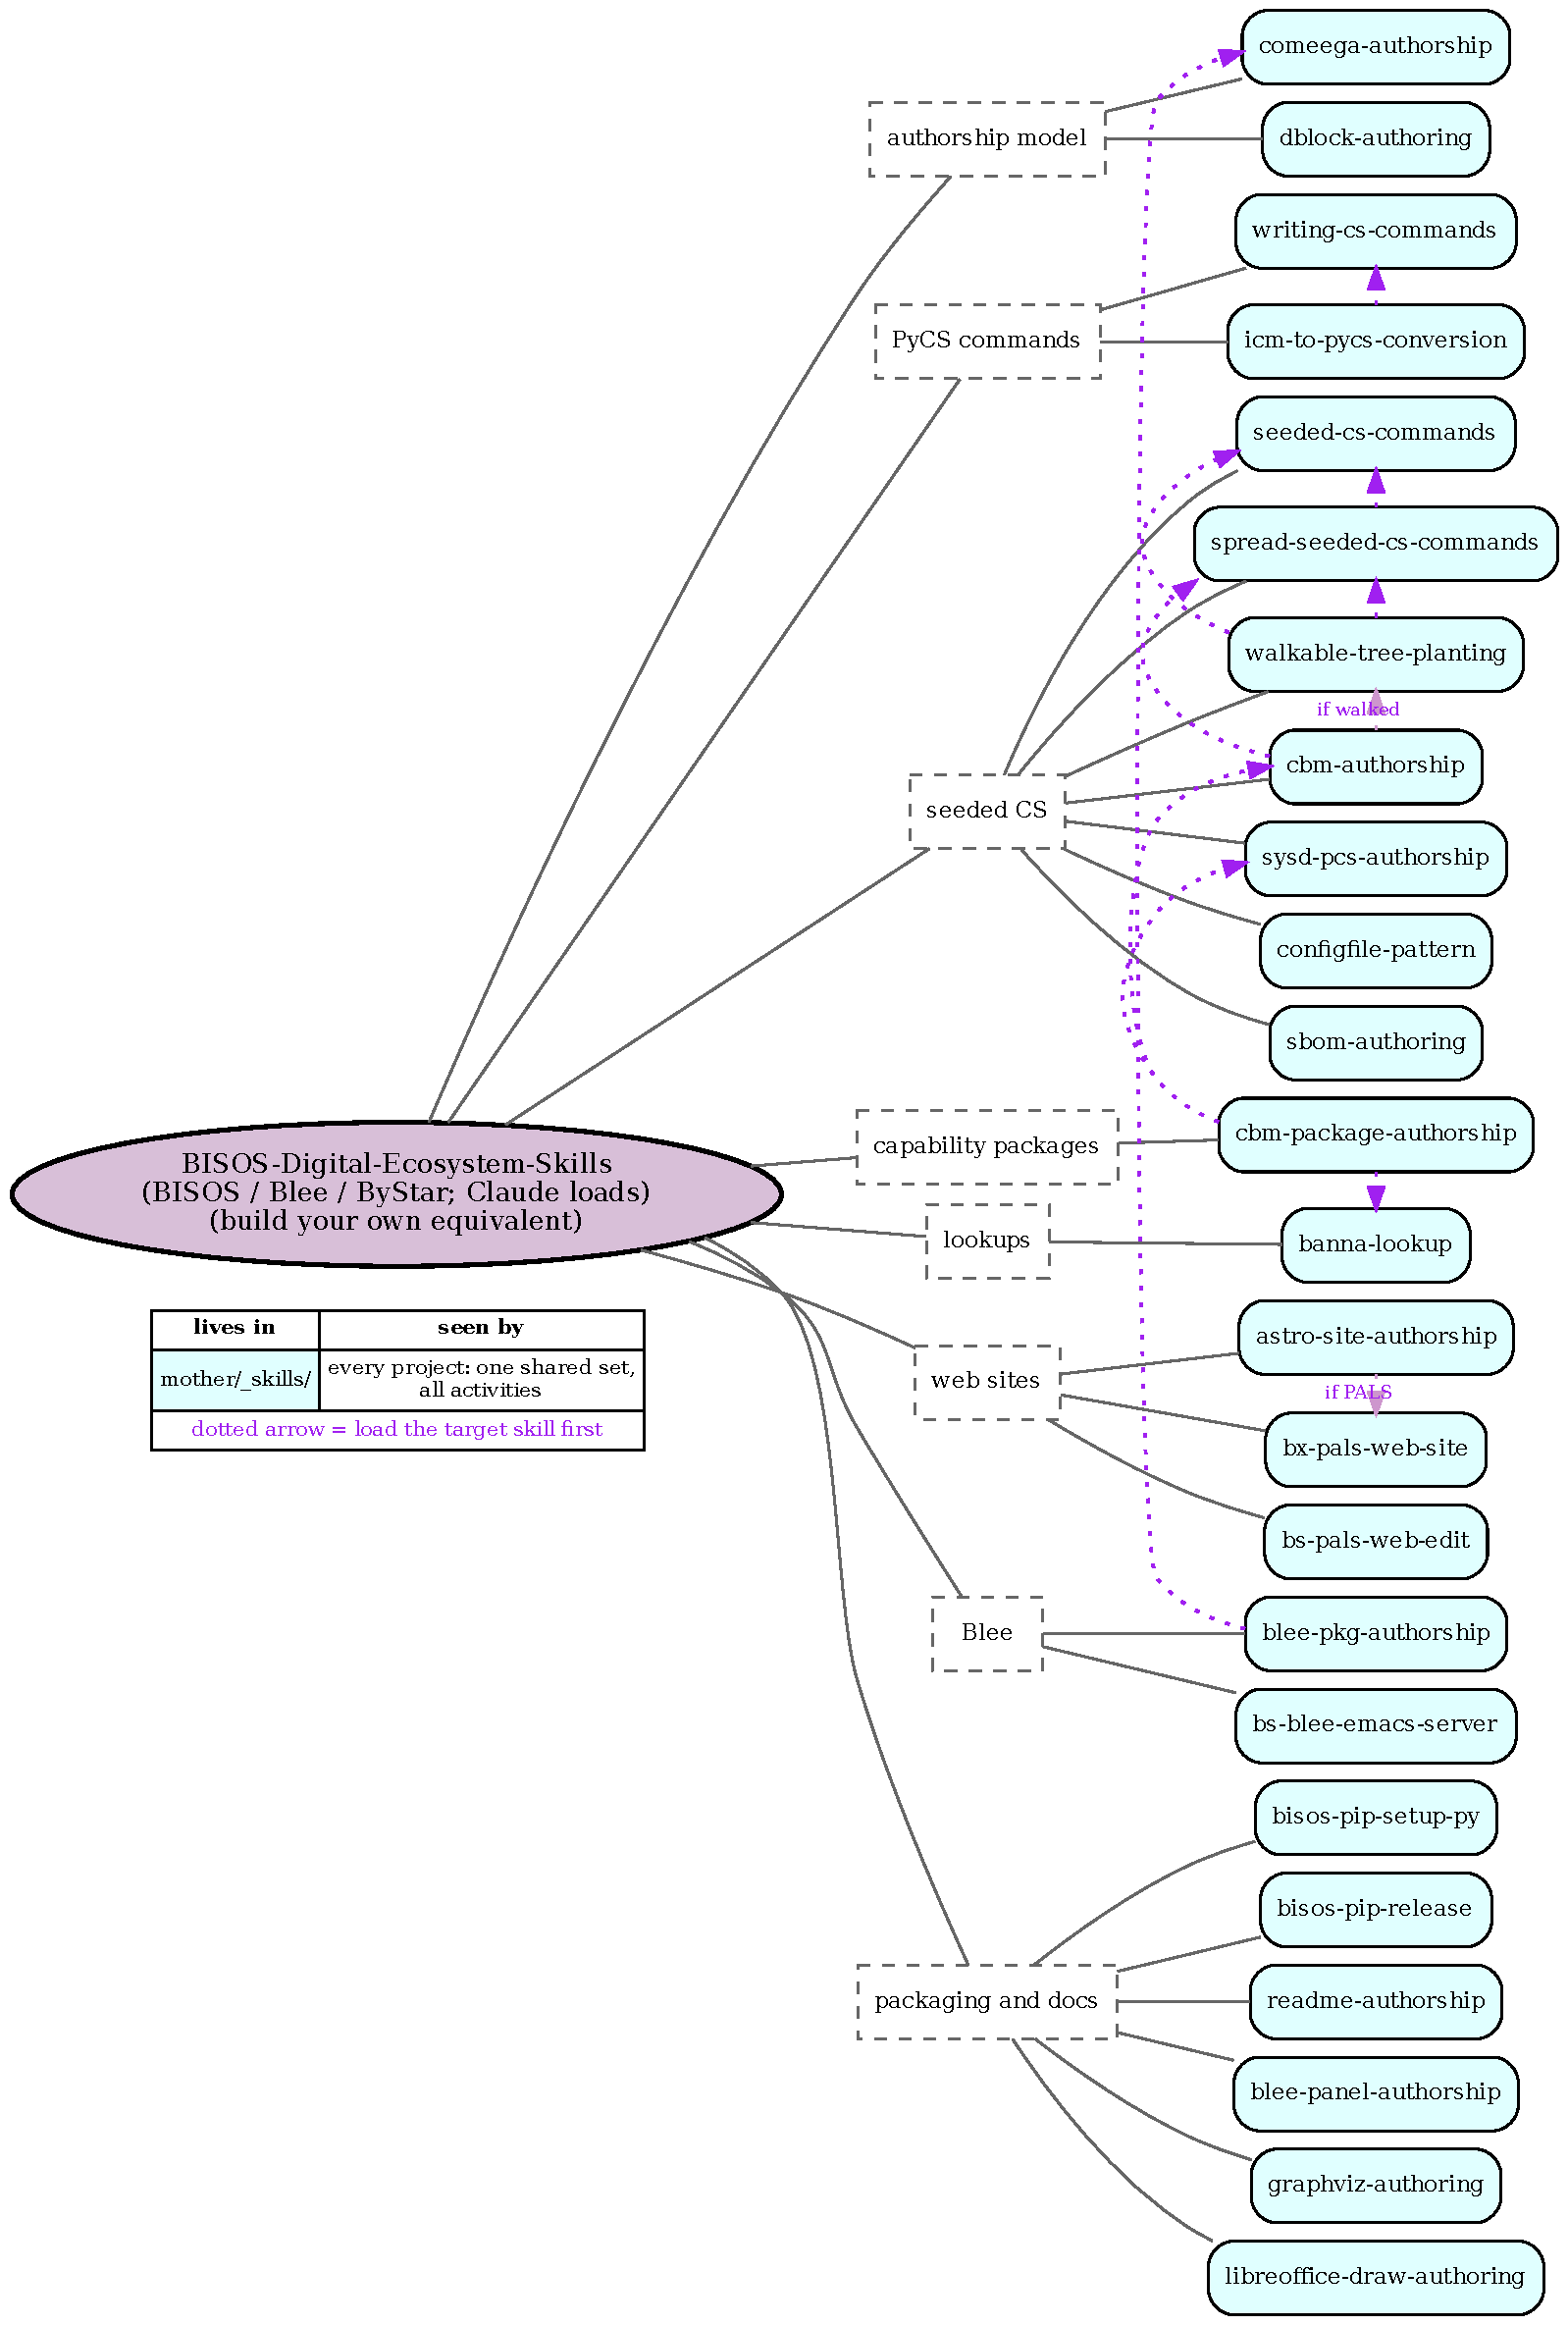
\includegraphics[width=\textwidth,height=0.98\textheight,keepaspectratio]{./figures/aiEcosystemTree}
  \end{center}
\end{latexonly}
\begin{htmlonly}
  \begin{rawhtml}
<div class="center">
<img src="./figures/aiEcosystemTree.png" height="450">
</div>
  \end{rawhtml}
\end{htmlonly}
\end{presentationMode}

\begin{articleMode}
  \begin{figure}[H]
    \begin{center}
      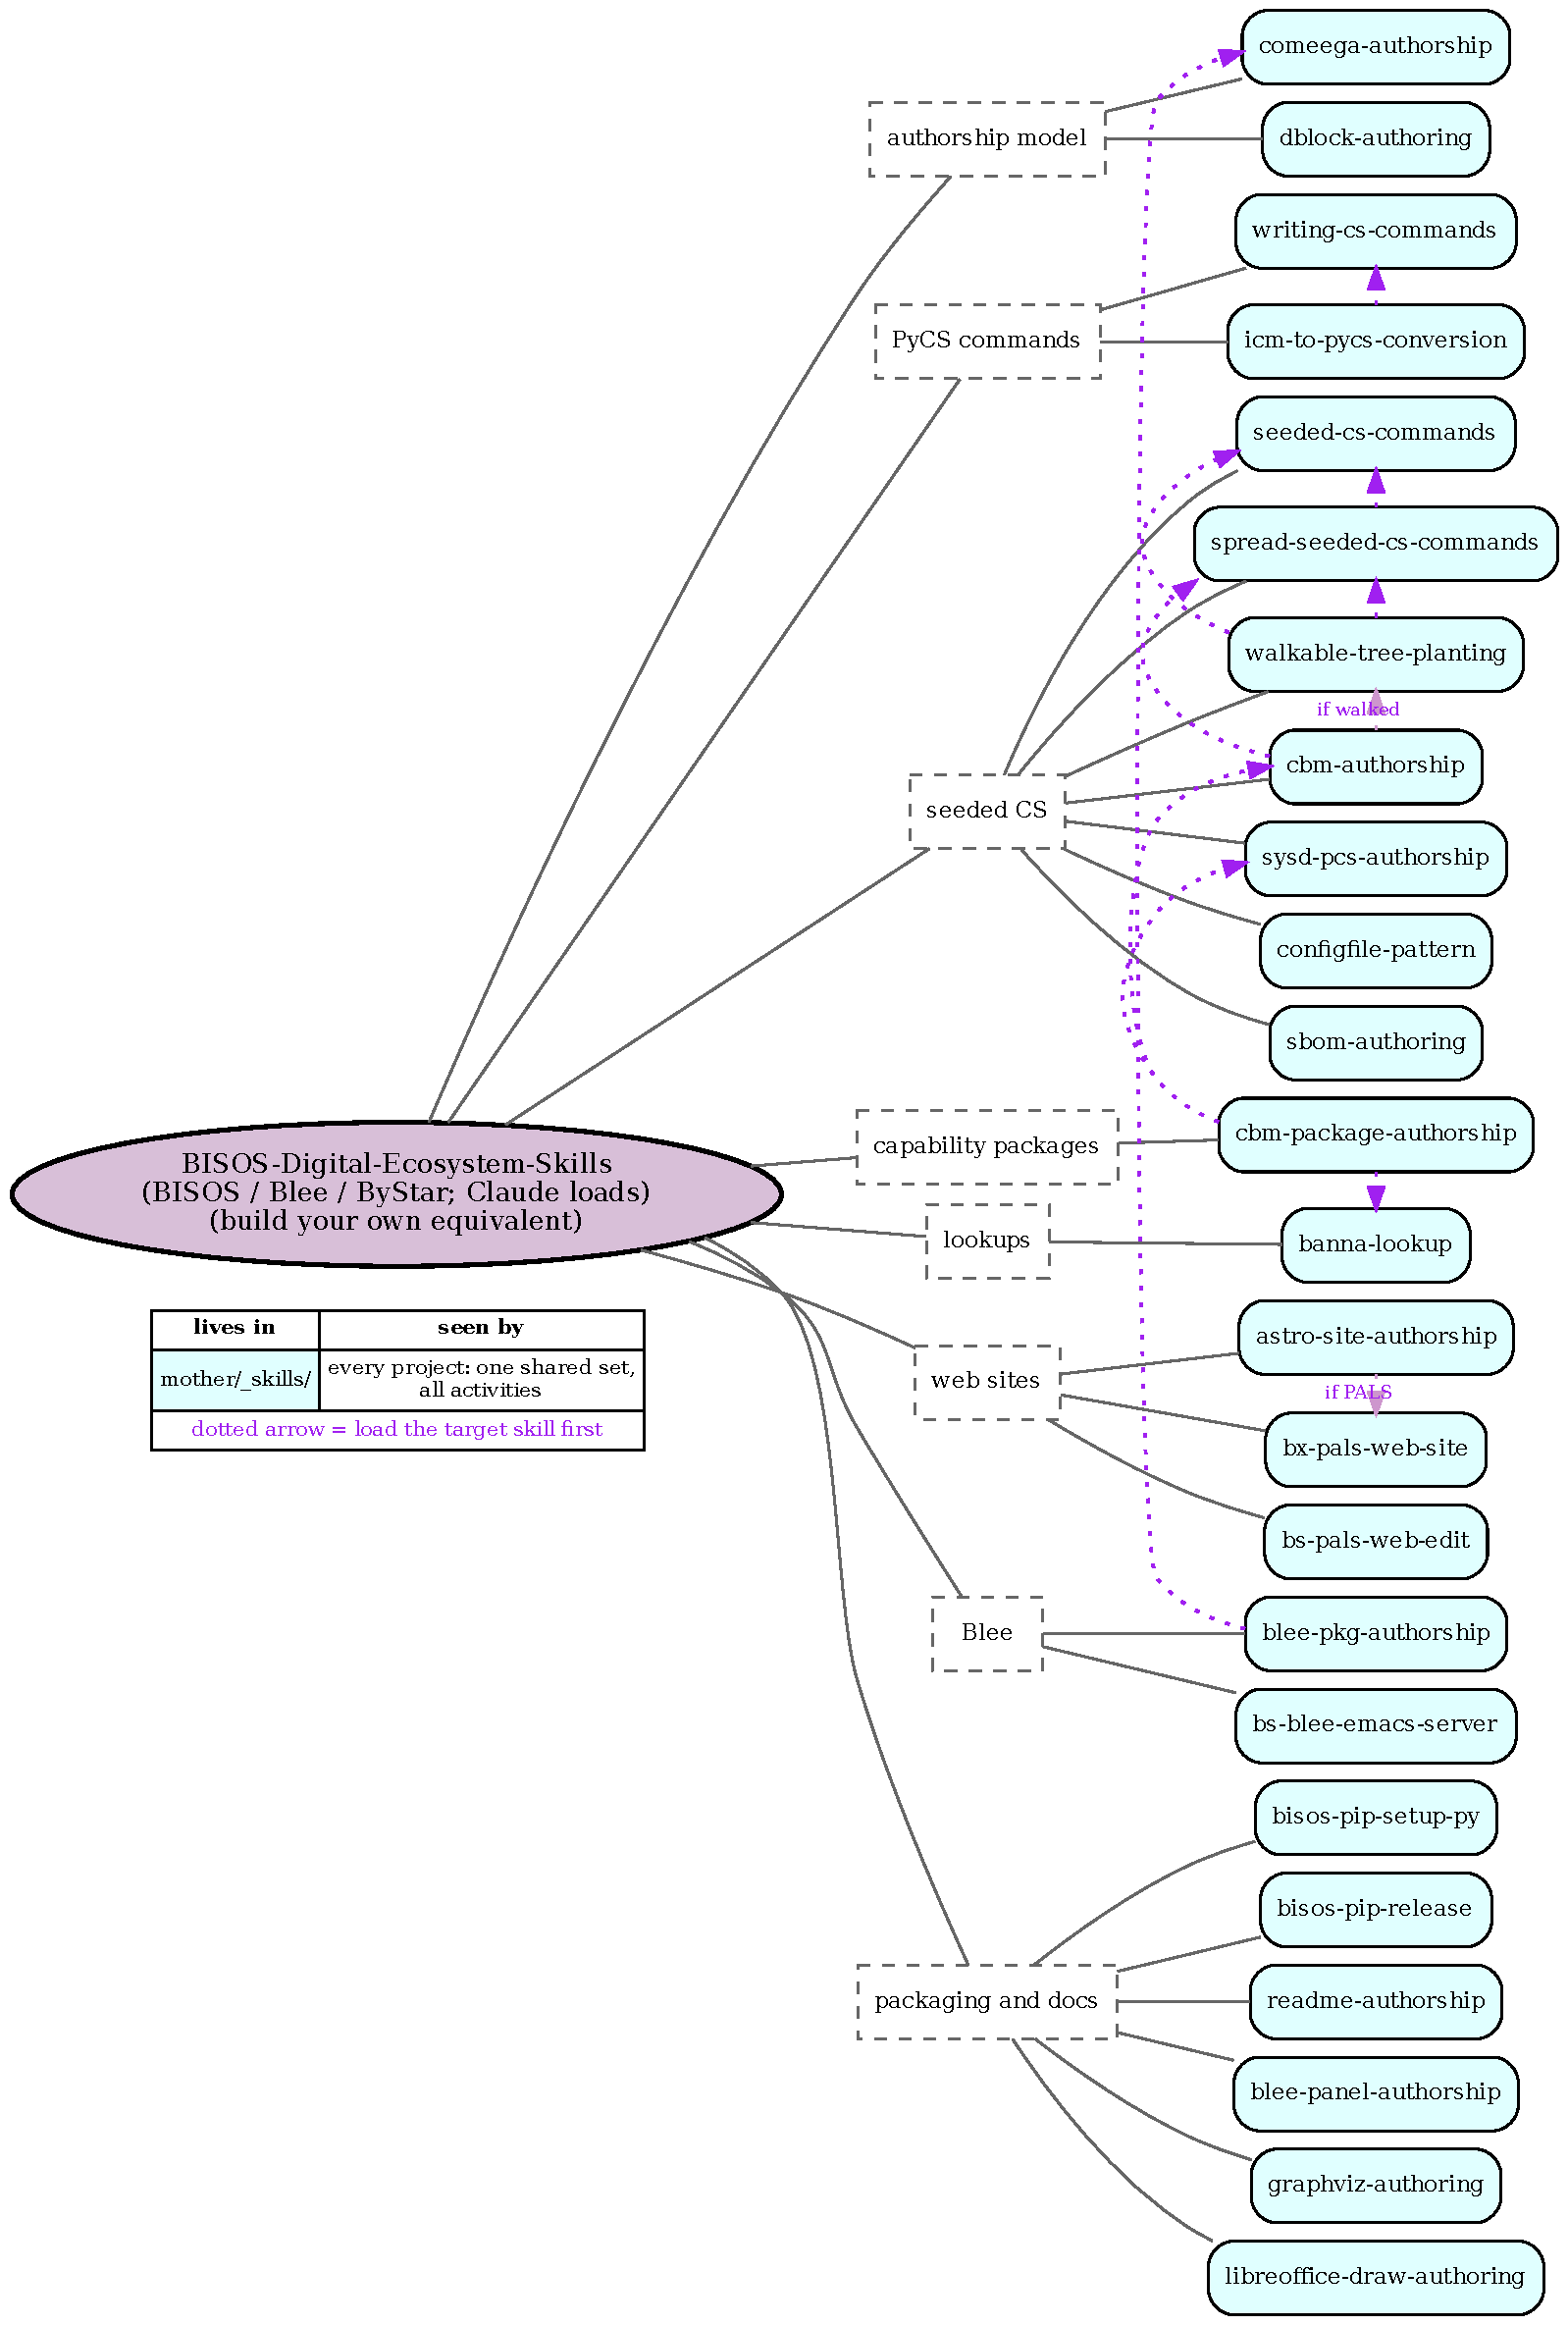
\includegraphics[width=\textwidth,height=0.8\textheight,keepaspectratio]{./figures/aiEcosystemTree}
      \caption{BISOS-Digital-Ecosystem-Skills}
      \label{fig:aiEcosystemTree}
    \end{center}
  \end{figure}
\end{articleMode}

\pnote{

These are the BISOS, Blee and ByStar skills, grouped by area.
Each one is a procedure that an AI loads when a task matches it.
Every lesson learned in one project becomes a line in a skill, for the next project.

}

\end{frame}
\end{verblatex}



%%%#+BEGIN: bx:dblock:lcnt:latex-section :mode "auto" :seg-title "Your Own Templates"
%%% Args: :class "book|pres+art" :langs "en+fa" :disabledP "false" :seg-title "str" :short-title "str" :label "auto"
\begin{whenOrg}
*  _[[elisp:(blee:menu-sel:outline:popupMenu)][±]]_ _[[elisp:(blee:menu-sel:navigation:popupMenu)][Ξ]]_ [[elisp:(outline-show-branches+toggle)][|=]] [[elisp:(bx:orgm:indirectBufOther)][|>]] *[[elisp:(blee:ppmm:org-mode-toggle)][|N]]*  Section    [[elisp:(outline-show-subtree+toggle)][||]]   /Your Own Templates/ ::  [[elisp:(org-cycle)][| ]]
\end{whenOrg}

\section{Your Own Templates}
%%%#+END:

%%%#+BEGIN: b:lcnt:pres:frame/derivedImage :title "Your Own Templates: Keep the Workflow, Replace the Skills" :subtitle "" :label "yourOwnTemplates" :comment "body=itemize" :reveal "plain" :beamer "plain"
\begin{whenOrg}
*****  _[[elisp:(blee:menu-sel:outline:popupMenu)][±]]_ _[[elisp:(blee:menu-sel:navigation:popupMenu)][Ξ]]_ [[elisp:(outline-show-branches+toggle)][|=]] [[elisp:(bx:orgm:indirectBufOther)][|>]] *[[elisp:(blee:ppmm:org-mode-toggle)][|N]]*  derivedImage [[elisp:(outline-show-subtree+toggle)][||]] Label=yourOwnTemplates Your Own Templates: Keep the Workflow, Replace the Skills body=itemize
\end{whenOrg}

\begin{htmlonly}

\begin{frame}[fragile,plain,label=yourOwnTemplates]
    \frameaudio{"audio/yourOwnTemplates.mp3"}
    \frametitle{}
    \framesubtitle{}
    \begin{rawhtml}
<div class="center">
<img src="./disposition.gened/yourOwnTemplates/slide-1.png" height="500">
</div>
    \end{rawhtml}
\end{frame}
\end{htmlonly}

\begin{verblatex}

\begin{frame}[fragile,plain,label=yourOwnTemplates]
    \frameaudio{"audio/yourOwnTemplates.mp3"}
    \frametitle{Your Own Templates: Keep the Workflow, Replace the Skills}
    \framesubtitle{}
%%BxPy: impressiveFrameParSet('yourOwnTemplates', 'always', 'True')
%%BxPy: impressiveFrameParSet('yourOwnTemplates', 'transition', 'UnSpecified')
%%%#+END:

\begin{itemize}
  \item The workflow: adopt as-is, at near-zero cost
  \item The ecosystem skills: build your own equivalent
    \begin{itemize}
    \item An Emacs package developer's conventions
    \item An organization's ways of doing things
    \end{itemize}
  \item None of ByStar/BISOS/Blee is a prerequisite
  \end{itemize}

\pnote{

To adopt this, keep the workflow, which costs almost nothing,
and replace the ecosystem skills with your own:
for example the conventions of Emacs package development.
None of ByStar, BISOS or Blee is a prerequisite.

}

\end{frame}
\end{verblatex}



%%%#+BEGIN: bx:dblock:lcnt:latex-part :disabledP "false" :seg-title "An Example Session"
%%% Args: :toc "NU" :tocDepth 3 :part "NU" :label "auto|spec" :partpage t
\begin{whenOrg}
*      ================
*  [[elisp:(blee:ppmm:org-mode-toggle)][|n]] [[elisp:(blee:menu-sel:outline:popupMenu)][+-]] [[elisp:(blee:menu-sel:navigation:popupMenu)][==]]  *Part*   _An Example Session_ ::  [[elisp:(org-cycle)][| ]]
\end{whenOrg}

\newpage
\part{An Example Session}
%%%#+END:

%%%#+BEGIN: bx:dblock:lcnt:latex-section :mode "auto" :seg-title "An Example Session, Recorded"
%%% Args: :class "book|pres+art" :langs "en+fa" :disabledP "false" :seg-title "str" :short-title "str" :label "auto"
\begin{whenOrg}
*  _[[elisp:(blee:menu-sel:outline:popupMenu)][±]]_ _[[elisp:(blee:menu-sel:navigation:popupMenu)][Ξ]]_ [[elisp:(outline-show-branches+toggle)][|=]] [[elisp:(bx:orgm:indirectBufOther)][|>]] *[[elisp:(blee:ppmm:org-mode-toggle)][|N]]*  Section    [[elisp:(outline-show-subtree+toggle)][||]]   /An Example Session, Recorded/ ::  [[elisp:(org-cycle)][| ]]
\end{whenOrg}

\section{An Example Session, Recorded}
%%%#+END:

%%%#+BEGIN: b:lcnt:pres:frame/derivedImage :title "An Example Session" :subtitle "" :label "exampleSession" :comment "body=video-placeholder" :reveal "plain" :beamer "plain"
\begin{whenOrg}
*****  _[[elisp:(blee:menu-sel:outline:popupMenu)][±]]_ _[[elisp:(blee:menu-sel:navigation:popupMenu)][Ξ]]_ [[elisp:(outline-show-branches+toggle)][|=]] [[elisp:(bx:orgm:indirectBufOther)][|>]] *[[elisp:(blee:ppmm:org-mode-toggle)][|N]]*  derivedImage [[elisp:(outline-show-subtree+toggle)][||]] Label=exampleSession An Example Session body=video-placeholder
\end{whenOrg}

\begin{htmlonly}

\begin{frame}[fragile,plain,label=exampleSession]
    \frameaudio{"audio/exampleSession.mp3"}
    \frametitle{}
    \framesubtitle{}
    \begin{rawhtml}
<div class="center">
<img src="./disposition.gened/exampleSession/slide-1.png" height="500">
</div>
    \end{rawhtml}
\end{frame}
\end{htmlonly}

\begin{verblatex}

\begin{frame}[fragile,plain,label=exampleSession]
    \frameaudio{"audio/exampleSession.mp3"}
    \frametitle{An Example Session}
    \framesubtitle{}
%%BxPy: impressiveFrameParSet('exampleSession', 'always', 'True')
%%BxPy: impressiveFrameParSet('exampleSession', 'transition', 'UnSpecified')
%%%#+END:

\begin{center}
    {\Large Video: an example session}\\
    \vspace{0.2in}
    (To be recorded)
  \end{center}

  \begin{itemize}
  \item Start a session at an AI-Activity Root
  \item Work a TODO from \texttt{AI-WorkPlan.org}
  \item Record the results and the status
  \item Commit, with an AI-written message
  \end{itemize}

\pnote{

Now let's look at an example session: starting at an AI-Activity root,
working a TODO from the work plan, recording the results and the status,
and committing.

}

\end{frame}
\end{verblatex}



%%%#+BEGIN: bx:dblock:lcnt:latex-part :disabledP "false" :seg-title "Observations and Closing"
%%% Args: :toc "NU" :tocDepth 3 :part "NU" :label "auto|spec" :partpage t
\begin{whenOrg}
*      ================
*  [[elisp:(blee:ppmm:org-mode-toggle)][|n]] [[elisp:(blee:menu-sel:outline:popupMenu)][+-]] [[elisp:(blee:menu-sel:navigation:popupMenu)][==]]  *Part*   _Observations and Closing_ ::  [[elisp:(org-cycle)][| ]]
\end{whenOrg}

\newpage
\part{Observations and Closing}
%%%#+END:

%%%#+BEGIN: bx:dblock:lcnt:latex-section :mode "auto" :seg-title "Observations on the Future of AI in Emacs"
%%% Args: :class "book|pres+art" :langs "en+fa" :disabledP "false" :seg-title "str" :short-title "str" :label "auto"
\begin{whenOrg}
*  _[[elisp:(blee:menu-sel:outline:popupMenu)][±]]_ _[[elisp:(blee:menu-sel:navigation:popupMenu)][Ξ]]_ [[elisp:(outline-show-branches+toggle)][|=]] [[elisp:(bx:orgm:indirectBufOther)][|>]] *[[elisp:(blee:ppmm:org-mode-toggle)][|N]]*  Section    [[elisp:(outline-show-subtree+toggle)][||]]   /Observations on the Future of AI in Emacs/ ::  [[elisp:(org-cycle)][| ]]
\end{whenOrg}

\section{Observations on the Future of AI in Emacs}
%%%#+END:

%%%#+BEGIN: b:lcnt:pres:frame/derivedImage :title "Some Observations on AI and AI Inside of Emacs" :subtitle "" :label "observations" :comment "body=itemize" :reveal "plain" :beamer "plain"
\begin{whenOrg}
*****  _[[elisp:(blee:menu-sel:outline:popupMenu)][±]]_ _[[elisp:(blee:menu-sel:navigation:popupMenu)][Ξ]]_ [[elisp:(outline-show-branches+toggle)][|=]] [[elisp:(bx:orgm:indirectBufOther)][|>]] *[[elisp:(blee:ppmm:org-mode-toggle)][|N]]*  derivedImage [[elisp:(outline-show-subtree+toggle)][||]] Label=observations Some Observations on AI and AI Inside of Emacs body=itemize
\end{whenOrg}

\begin{htmlonly}

\begin{frame}[fragile,plain,label=observations]
    \frameaudio{"audio/observations.mp3"}
    \frametitle{}
    \framesubtitle{}
    \begin{rawhtml}
<div class="center">
<img src="./disposition.gened/observations/slide-1.png" height="500">
</div>
    \end{rawhtml}
\end{frame}
\end{htmlonly}

\begin{verblatex}

\begin{frame}[fragile,plain,label=observations]
    \frameaudio{"audio/observations.mp3"}
    \frametitle{Some Observations on AI and AI Inside of Emacs}
    \framesubtitle{}
%%BxPy: impressiveFrameParSet('observations', 'always', 'True')
%%BxPy: impressiveFrameParSet('observations', 'transition', 'UnSpecified')
%%%#+END:

\begin{itemize}
  \item Value shifts from code to the context that produces it
  \item Who owns the workflow matters: the user or the vendor
  \item The editor becomes the place where the context lives
  \item Emacs, omni-moded and convivial, is a natural host
  \item We are early: none of us has figured out the right way yet
  \end{itemize}

\pnote{

A few observations. Value is shifting from code to the context that produces it.
Who owns that workflow, the user or the vendor, matters.
Emacs, omni-moded and convivial, is a natural host for it.
And we are early; none of us can claim to have figured out the right way yet.

}

\end{frame}
\end{verblatex}



%%%#+BEGIN: bx:dblock:lcnt:latex-section :mode "auto" :seg-title "Try It, Adapt It"
%%% Args: :class "book|pres+art" :langs "en+fa" :disabledP "false" :seg-title "str" :short-title "str" :label "auto"
\begin{whenOrg}
*  _[[elisp:(blee:menu-sel:outline:popupMenu)][±]]_ _[[elisp:(blee:menu-sel:navigation:popupMenu)][Ξ]]_ [[elisp:(outline-show-branches+toggle)][|=]] [[elisp:(bx:orgm:indirectBufOther)][|>]] *[[elisp:(blee:ppmm:org-mode-toggle)][|N]]*  Section    [[elisp:(outline-show-subtree+toggle)][||]]   /Try It, Adapt It/ ::  [[elisp:(org-cycle)][| ]]
\end{whenOrg}

\section{Try It, Adapt It}
%%%#+END:

%%%#+BEGIN: b:lcnt:pres:frame/derivedImage :title "Try It, Adapt It" :subtitle "" :label "tryIt" :comment "body=itemize" :reveal "plain" :beamer "plain"
\begin{whenOrg}
*****  _[[elisp:(blee:menu-sel:outline:popupMenu)][±]]_ _[[elisp:(blee:menu-sel:navigation:popupMenu)][Ξ]]_ [[elisp:(outline-show-branches+toggle)][|=]] [[elisp:(bx:orgm:indirectBufOther)][|>]] *[[elisp:(blee:ppmm:org-mode-toggle)][|N]]*  derivedImage [[elisp:(outline-show-subtree+toggle)][||]] Label=tryIt Try It, Adapt It body=itemize
\end{whenOrg}

\begin{htmlonly}

\begin{frame}[fragile,plain,label=tryIt]
    \frameaudio{"audio/tryIt.mp3"}
    \frametitle{}
    \framesubtitle{}
    \begin{rawhtml}
<div class="center">
<img src="./disposition.gened/tryIt/slide-1.png" height="500">
</div>
    \end{rawhtml}
\end{frame}
\end{htmlonly}

\begin{verblatex}

\begin{frame}[fragile,plain,label=tryIt]
    \frameaudio{"audio/tryIt.mp3"}
    \frametitle{Try It, Adapt It}
    \framesubtitle{}
%%BxPy: impressiveFrameParSet('tryIt', 'always', 'True')
%%BxPy: impressiveFrameParSet('tryIt', 'transition', 'UnSpecified')
%%%#+END:

\begin{itemize}
  \item \texttt{pipx install bisos.aiActivity}
  \item \href{https://github.com/bisos-pip/aiActivity}{https://github.com/bisos-pip/aiActivity}
  \item \href{https://github.com/bxObjects/aiActivityTemplates}{https://github.com/bxObjects/aiActivityTemplates}
  \item \href{https://github.com/bx-blee/vscode-claude}{https://github.com/bx-blee/vscode-claude}
  \end{itemize}

  \vspace{0.15in}
  Take the templates, adapt them --- and if you try it, let me know what breaks.

\pnote{

Take the templates and adapt them.
And if you try it, let me know what breaks.

}

\end{frame}
\end{verblatex}



%%%#+BEGIN: bx:dblock:lcnt:latex-section :mode "auto" :seg-title "Thanks"
%%% Args: :class "book|pres+art" :langs "en+fa" :disabledP "false" :seg-title "str" :short-title "str" :label "auto"
\begin{whenOrg}
*  _[[elisp:(blee:menu-sel:outline:popupMenu)][±]]_ _[[elisp:(blee:menu-sel:navigation:popupMenu)][Ξ]]_ [[elisp:(outline-show-branches+toggle)][|=]] [[elisp:(bx:orgm:indirectBufOther)][|>]] *[[elisp:(blee:ppmm:org-mode-toggle)][|N]]*  Section    [[elisp:(outline-show-subtree+toggle)][||]]   /Thanks/ ::  [[elisp:(org-cycle)][| ]]
\end{whenOrg}

\section{Thanks}
%%%#+END:

%%%#+BEGIN: b:lcnt:pres:frame/derivedImage :title "Thanks" :subtitle "" :label "thanks" :comment "body=itemize" :reveal "plain" :beamer "plain"
\begin{whenOrg}
*****  _[[elisp:(blee:menu-sel:outline:popupMenu)][±]]_ _[[elisp:(blee:menu-sel:navigation:popupMenu)][Ξ]]_ [[elisp:(outline-show-branches+toggle)][|=]] [[elisp:(bx:orgm:indirectBufOther)][|>]] *[[elisp:(blee:ppmm:org-mode-toggle)][|N]]*  derivedImage [[elisp:(outline-show-subtree+toggle)][||]] Label=thanks Thanks body=itemize
\end{whenOrg}

\begin{htmlonly}

\begin{frame}[fragile,plain,label=thanks]
    \frameaudio{"audio/thanks.mp3"}
    \frametitle{}
    \framesubtitle{}
    \begin{rawhtml}
<div class="center">
<img src="./disposition.gened/thanks/slide-1.png" height="500">
</div>
    \end{rawhtml}
\end{frame}
\end{htmlonly}

\begin{verblatex}

\begin{frame}[fragile,plain,label=thanks]
    \frameaudio{"audio/thanks.mp3"}
    \frametitle{Thanks}
    \framesubtitle{}
%%BxPy: impressiveFrameParSet('thanks', 'always', 'True')
%%BxPy: impressiveFrameParSet('thanks', 'transition', 'UnSpecified')
%%%#+END:

\begin{center}
    {\Large Thanks to the EmacsConf 2026 organizers}\\
    \vspace{0.2in}
    {\Large and to Sacha in particular.}
  \end{center}

\pnote{

I want to thank all the EmacsConf 2026 organizers for their great work.
And Sacha in particular.

}

\end{frame}
\end{verblatex}



\begin{comment}
*  [[elisp:(org-cycle)][| ]]  Local Vars  ::                  *Org-Mode And Emacs Specific Configurations*   [[elisp:(org-cycle)][| ]]
\end{comment}

%% Local Variables:
%% major-mode: latex-mode
%% fill-column: 90
%% End:
